\documentclass[12pt,a4paper,oneside]{report}

% ===================== ENCODAGE ET LANGUE =====================
\usepackage[utf8]{inputenc}
\usepackage[T1]{fontenc}
\usepackage[french]{babel}

% ===================== MISE EN PAGE =====================
\usepackage[a4paper,margin=2.5cm]{geometry}
\usepackage{setspace}
\onehalfspacing

% ===================== OUTILS =====================
\usepackage{tikz}
\usepackage{graphicx}
\usepackage{amsmath,amssymb}
\usepackage{hyperref}
\usepackage{fancyhdr}
\usepackage{tocloft}
\usepackage{titlesec}
\usepackage{array}
\usepackage{longtable}
\usepackage{caption}
\usepackage{float}
\usepackage{placeins}
\usepackage{xcolor}

% ===================== HYPERREF =====================
\hypersetup{
    colorlinks=true,
    linkcolor=black,
    citecolor=black,
    urlcolor=blue,
    pdftitle={Rapport PFE},
    pdfauthor={Ranim Khemir et Molka Hammami}
}

% ===================== HEADER / FOOTER =====================
\pagestyle{fancy}
\fancyhf{}

\fancyfoot[L]{\small Institut Supérieur des Arts Multimédia de la Manouba}
\fancyfoot[R]{\thepage}

\renewcommand{\headrulewidth}{0pt}
\renewcommand{\footrulewidth}{0.4pt}

\fancypagestyle{plain}{
    \fancyhf{}
    \fancyfoot[L]{\small Institut Supérieur des Arts Multimédia de la Manouba}
    \fancyfoot[R]{\thepage}
    \renewcommand{\headrulewidth}{0pt}
    \renewcommand{\footrulewidth}{0.4pt}
}

% ===================== STYLE DES TITRES =====================
\titleformat{\chapter}[display]
  {\bfseries\Large}
  {\filcenter\chaptername\ \thechapter}
  {1ex}
  {\filcenter}

% ===================== STYLE TABLE DES MATIERES =====================
\renewcommand{\contentsname}{}
\renewcommand{\listfigurename}{}
\renewcommand{\listtablename}{}

\renewcommand{\cftchapfont}{\bfseries}
\renewcommand{\cftchappagefont}{\bfseries}
\setlength{\cftbeforechapskip}{8pt}
\setlength{\cftbeforesecskip}{2pt}
\renewcommand{\cftdotsep}{1.5}
\setlength{\cftchapnumwidth}{3em}
\setlength{\cftsecindent}{2em}

\begin{document}

% ===================== PAGE DE GARDE =====================
\begin{titlepage}
\thispagestyle{empty}

\begin{tikzpicture}[remember picture,overlay]
    % Cadre en haut à droite
    \draw[line width=0.4pt]
    ([xshift=-2cm,yshift=-1.2cm]current page.north east)
    rectangle
    ([xshift=-7.3cm,yshift=-3.0cm]current page.north east);

    \node[anchor=north west,font=\bfseries\small]
    at ([xshift=-6.1cm,yshift=-1.45cm]current page.north east)
    {Code PFE : .....};
\end{tikzpicture}

\begin{center}

\vspace*{0.7cm}

{\bfseries\large Ministère de l’Enseignement Supérieur et de la Recherche\\ Scientifique}

\vspace{0.6cm}

{\bfseries\large Université de la Manouba}

\vspace{0.6cm}

{\bfseries\large Institut supérieur des Arts Multimédias }

\vspace{1cm}


\includegraphics[width=0.28\textwidth]{logo-isamm.png}

\vspace{0.4cm}

{\Large Rapport de projet de fin d’études}

\vspace{0.5cm}

{\normalsize Préparé pour l’obtention du diplôme de Licence en Informatique et Multimédia}

\vspace{0.9cm}

\noindent\rule{0.72\textwidth}{0.5pt}

\vspace{0.4cm}

{\bfseries\Large Plateforme intelligente de collecte et de gestion des réclamations}

\vspace{0.4cm}

\noindent\rule{0.72\textwidth}{0.5pt}

\vspace{0.5cm}

{\bfseries\large Réalisé par}

\vspace{0.35cm}

{\normalsize Khemir Ranim \\ Hammami Molka}

\vspace{0.5cm}

{\bfseries\large Encadré par}

\vspace{0.35cm}

{\normalsize Mme Falleh Meriem - ISAMM}

\vspace{0.2cm}

{\normalsize Mme Terzi Emna - MAE assurances \\M. Mohamed Salah Farah - MAE assurances}

\vfill
\vspace{0.8cm}

{\normalsize Année universitaire : 2025/2026}

\end{center}
\end{titlepage}
% ===================== PAGES PRELIMINAIRES =====================
\pagenumbering{roman}

% ===== DEDICACE =====
\chapter*{Dédicace}

Je dédie ce travail à ma famille, pour son soutien, sa patience et ses encouragements tout au long de ce parcours.

\clearpage

% ===== REMERCIEMENTS =====
\chapter*{Remerciements}



\clearpage

% ===== RESUME =====
\chapter*{Résumé}
Ce projet de fin d’études porte sur la conception et le développement d’une plateforme intelligente de collecte et de gestion des réclamations clients pour MAE Assurances. La solution proposée permet de collecter des commentaires issus de sources telles que Facebook et LinkedIn, de les nettoyer, de les centraliser dans une base de données PostgreSQL et de les analyser automatiquement à l’aide d’un module NLP.

La plateforme repose sur une architecture composée d’une interface web développée avec React, d’un backend Django REST Framework, d’une base de données PostgreSQL et d’un module intelligent combinant des modèles de Machine Learning, un LLM et un mécanisme LLM-as-a-Judge. Cette approche hybride permet de détecter les réclamations, de classifier leur catégorie, d’estimer leur niveau d’urgence et de valider les cas incertains.

Un dashboard BI a également été intégré afin de visualiser les indicateurs clés, suivre l’état des réclamations et faciliter la prise de décision. Les tests réalisés sur les modèles, le module NLP et les API backend montrent que la solution permet d’automatiser une partie importante du traitement des réclamations tout en gardant la possibilité d’une intervention humaine pour les cas non classés ou ambigus.

\textbf{Mots-clés :} Réclamations clients, NLP, Machine Learning, LLM, LLM-as-a-Judge, Django, React, PostgreSQL, Dashboard BI.



\clearpage

% ===== ABSTRACT =====
\chapter*{Abstract}

This final year project focuses on the design and development of an intelligent platform for collecting and managing customer complaints for MAE Assurances. The proposed solution collects comments from sources such as Facebook and LinkedIn, cleans and centralizes them in a PostgreSQL database, and analyzes them automatically using a Natural Language Processing (NLP) module.

The platform is based on a modular architecture composed of a web interface developed with React, a backend built with Django REST Framework, a PostgreSQL database, and an intelligent module combining Machine Learning models, a Large Language Model (LLM), and an LLM-as-a-Judge validation mechanism. This hybrid approach makes it possible to detect complaints, classify them by category, estimate their urgency level, and validate uncertain or ambiguous cases.

A BI dashboard was also integrated to visualize key indicators, monitor the status of complaints, and support decision-making. The tests carried out on the ML models, the NLP module, and the backend APIs show that the solution can automate an important part of complaint processing while keeping the possibility of human intervention for unclassified or uncertain cases.

\textbf{Keywords:} customer complaints, NLP, Machine Learning, LLM, LLM-as-a-Judge, Django, React, PostgreSQL, BI dashboard.

\clearpage

% ===== TABLE DES MATIERES =====
\tableofcontents
\clearpage

% ===== LISTE DES FIGURES =====
\chapter*{Liste des figures}
\listoffigures
\clearpage

% ===== LISTE DES TABLEAUX =====
\chapter*{Liste des tableaux}
\listoftables
\clearpage

% ===== LISTE DES ABREVIATIONS =====
\chapter*{Liste des abréviations}
\begin{tabular}{>{\bfseries}p{3cm} p{10cm}}
API & Application Programming Interface \\
REST & Representational State Transfer \\
JSON & JavaScript Object Notation \\
JWT & JSON Web Token \\
HTTP & HyperText Transfer Protocol \\
URL & Uniform Resource Locator \\
CRUD & Create, Read, Update, Delete \\
ORM & Object Relational Mapping \\
DB & Database \\
SQL & Structured Query Language \\
BI & Business Intelligence \\
CRISP-DM & Cross-Industry Standard Process for Data Mining \\
NLP & Natural Language Processing \\
KPI & Key Performance Indicator \\
UML & Unified Modeling Language \\
ML & Machine Learning \\
LLM & Large Language Model \\
CORS & Cross-Origin Resource Sharing \\
\end{tabular}
\clearpage

% ===================== CORPS DU RAPPORT =====================
\pagenumbering{arabic}

% ===== INTRODUCTION GENERALE =====
\chapter*{Introduction générale}
\addcontentsline{toc}{chapter}{Introduction générale}

Ces dernières années, la relation entre les entreprises et leurs clients a connu une évolution importante avec la multiplication des canaux numériques. Les clients expriment désormais leurs avis, demandes et réclamations à travers différents supports, notamment les réseaux sociaux, les courriels et les plateformes en ligne. Ces données constituent une source d’information précieuse pour comprendre les attentes des clients, améliorer la qualité du service et renforcer la prise de décision.

Dans le secteur des assurances, la gestion des réclamations occupe une place essentielle, car elle permet de suivre les insatisfactions des clients, d’identifier les problèmes récurrents et d’améliorer la qualité des services. \textbf{MAE Assurances}, en tant qu’entreprise opérant dans ce domaine, reçoit des retours et des demandes à travers différents canaux numériques. Le traitement de ces informations devient alors un enjeu important pour assurer un meilleur suivi des clients.

Cependant, la gestion manuelle des réclamations devient de plus en plus complexe lorsque le volume des commentaires augmente. Les données collectées sont souvent non structurées, rédigées sous forme de texte libre et peuvent contenir plusieurs langues, des abréviations ou des formulations ambiguës. Cette situation rend difficile l’identification rapide des réclamations, leur classification par catégorie et la détection des cas urgents.

Ce projet vise donc à concevoir et développer une plateforme intelligente de collecte, d’analyse et de gestion des réclamations clients pour MAE Assurances. La solution proposée permet de centraliser les commentaires collectés, de les nettoyer, de les analyser automatiquement à l’aide d’un module NLP et de faciliter leur suivi à travers une interface web.

Les principales contributions de ce projet sont les suivantes :

\begin{itemize}
    \item la collecte et la préparation des commentaires issus de sources numériques telles que \textbf{Facebook} et \textbf{LinkedIn} ;
    \item la mise en place d’un \textbf{module NLP hybride} combinant des modèles de \textbf{Machine Learning}, un \textbf{LLM} et un mécanisme \textbf{LLM-as-a-Judge} ;
    \item le développement d’un backend basé sur \textbf{Django REST Framework }pour la gestion des utilisateurs, des réclamations et des API ;
    \item la conception d’une interface web avec \textbf{React} permettant aux agents et à l’administrateur de consulter, filtrer, traiter et suivre les réclamations ;
    \item l’intégration d’un \textbf{dashboard BI} pour visualiser les indicateurs clés et faciliter la prise de décision.
\end{itemize}

Pour organiser la réalisation du projet, nous avons adopté la méthodologie \textbf{CRISP-DM}, qui propose une démarche structurée allant de la compréhension du besoin métier jusqu’à l’exploitation des résultats.

Ce rapport est organisé en plusieurs chapitres. Le premier chapitre présente le contexte général du projet et la compréhension métier. Le deuxième chapitre est consacré à l’analyse des besoins et à la spécification. Le troisième chapitre décrit la conception globale de la solution. Le quatrième chapitre présente la collecte et la préparation des données. Le cinquième chapitre détaille le développement du backend et de la base de données. Le sixième chapitre présente le frontend ainsi que les mécanismes de sécurité. Enfin, le dernier chapitre est consacré au traitement intelligent des réclamations, à l’analyse des résultats, aux KPI et au dashboard BI.


% ===== CHAPITRE 1 =====
\chapter{Contexte général et compréhension métier}

\section{Introduction}
Dans ce chapitre, nous présentons le cadre général du projet ainsi que son contexte métier. Nous exposons l’entreprise d’accueil, le domaine des réclamations clients, les limites des approches traditionnelles et les raisons ayant motivé la mise en place d’une solution intelligente.

\section{Présentation de l’entreprise}

Dans le cadre de ce projet de fin d’études, nous avons réalisé notre stage au sein de la société \textbf{MAE Assurances}, une entreprise opérant dans le domaine des assurances en Tunisie.

La MAE (Mutuelle Assurance de l’Enseignement) est une société mutualiste fondée en 1962. Elle a été créée dans le but d’établir un lien de solidarité entre ses adhérents et de leur offrir une protection contre différents types de risques \cite{mae}. Au fil du temps, elle a élargi ses services pour couvrir plusieurs domaines liés à la vie quotidienne.

La MAE est spécialisée dans la protection des individus et des biens, particulièrement dans les secteurs liés à l'éducation, à la famille et à la vie courante. Elle propose différents produits d'assurance répondant aux besoins de ses clients, tels que l'assurance scolaire, l'assurance habitation et la responsabilité civile.

La société accorde une importance particulière à la qualité de ses prestations et à la satisfaction de sa clientèle. Dans ce contexte, la gestion des réclamations représente un aspect essentiel, car elle permet d’identifier les problèmes rencontrés par les clients et d’améliorer les services proposés.

Avec l’avancée des technologies numériques et la multiplication des moyens de communication (emails, réseaux sociaux, sites web), la MAE fait face à une augmentation constante du nombre de réclamations. Ces données, souvent sous forme de texte non structuré, rendent leur traitement plus complexe et nécessitent l’utilisation de solutions innovantes et automatisées.

C’est dans ce cadre que s’inscrit ce projet, ayant pour objectif de concevoir et de développer une plateforme intelligente capable de collecter, analyser et exploiter les réclamations des clients, afin d’améliorer la qualité du service et de faciliter la prise de décision \cite{mae}.


\begin{figure}[H]
    \centering
    
\includegraphics[width=0.25\textwidth]{mae.png}
    \caption{Logo de MAE}
\end{figure}
\section{Présentation du domaine}

Le domaine des réclamations clients joue un rôle très important dans les entreprises, en particulier dans le secteur des services comme les assurances. Une réclamation correspond à une insatisfaction exprimée par un client suite à un problème rencontré avec un service ou un produit.

Avec le développement des technologies numériques, les entreprises reçoivent aujourd’hui un grand nombre de réclamations provenant de différentes sources, telles que les emails, les sites web, les réseaux sociaux ou encore les applications en ligne. Cette diversité des canaux rend la gestion des réclamations plus complexe.

La majorité des réclamations sont sous forme de texte libre, ce qui signifie qu’elles ne sont pas structurées. Cela complique leur analyse et nécessite souvent un traitement manuel long et inefficace. De plus, il devient difficile d’identifier rapidement les réclamations urgentes ou les problèmes les plus fréquents.

Pour faire face à ces défis, les entreprises adoptent de plus en plus des solutions basées sur l’intelligence artificielle, notamment le traitement automatique du langage naturel (NLP). Ces techniques permettent de traiter automatiquement les réclamations, de les classer selon leur catégorie et d’identifier les cas urgents \cite{ibmnlp}.

Dans ce contexte, la mise en place d’une plateforme intelligente de gestion des réclamations permet d’améliorer l’efficacité du traitement, de réduire les délais de réponse et d’aider les entreprises à prendre de meilleures décisions.

\section{Gestion traditionnelle des réclamations}

Dans les entreprises, la gestion des réclamations clients se fait généralement de manière traditionnelle à l’aide de méthodes manuelles ou d’outils simples. Les réclamations sont souvent reçues à travers différents canaux comme les emails, les appels téléphoniques ou les formulaires en ligne.

Dans ce type de gestion, les agents traitent les réclamations une par une. Ils lisent le contenu, identifient le problème, puis enregistrent les informations dans un système ou un fichier. Ce processus dépend fortement de l’intervention humaine, ce qui peut prendre du temps et entraîner des erreurs.

De plus, le classement des réclamations est souvent effectué manuellement. Cela rend difficile l’organisation des données et complique la recherche d’informations. Il devient aussi compliqué de détecter rapidement les réclamations urgentes ou les problèmes les plus fréquents.



Ainsi, la gestion traditionnelle des réclamations montre ses limites face à l’augmentation du volume de données et à la diversité des sources. Cela met en évidence la nécessité d’adopter des solutions plus modernes et automatisées pour améliorer l’efficacité et la qualité du service.

\section{Problématique détaillée}

Avec la multiplication des canaux de communication numériques, les entreprises reçoivent un volume croissant de commentaires, d’avis et de réclamations provenant de sources variées. Dans le cadre de ce projet, le dataset exploité contient plusieurs centaines de commentaires, ce qui rend leur traitement manuel long, répétitif et difficile à maintenir.

Les réclamations sont généralement rédigées sous forme de texte libre. Elles peuvent contenir des fautes, des abréviations, des formulations ambiguës ou plusieurs langues. Cette nature non structurée complique leur analyse automatique et oblige souvent les agents à lire chaque commentaire afin d’identifier s’il s’agit réellement d’une réclamation.

Un autre problème concerne la classification et la priorisation. Sans mécanisme intelligent, il devient difficile de classer rapidement les réclamations selon leur catégorie, par exemple Service Client, Sinistre Auto, Sinistre IRDS ou Sinistre Vie. De plus, les cas urgents peuvent être noyés parmi des demandes simples ou des commentaires non réclamants, ce qui peut entraîner des retards de traitement et affecter la satisfaction des clients.

Enfin, l’absence d’outils de visualisation limite l’exploitation des données collectées. Les responsables ne disposent pas toujours d’indicateurs clairs permettant de suivre le nombre de réclamations, leur évolution, leur statut ou leur répartition par catégorie et par niveau d’urgence.

Dans ce contexte, la problématique principale de ce projet peut être formulée comme suit :

\textbf{Comment concevoir une plateforme intelligente capable de collecter, classifier et prioriser automatiquement les réclamations clients, tout en facilitant leur suivi et leur analyse à travers des indicateurs visuels ?}

\section{Étude de l’existant}

Avant de proposer une solution adaptée, il est nécessaire d’analyser les outils existants dédiés à la gestion des réclamations et du support client. Parmi les solutions les plus connues, on peut citer \textbf{Zendesk}, \textbf{Salesforce Service Cloud} et \textbf{Freshdesk}. Ces plateformes permettent de centraliser les demandes clients, de gérer des tickets, de suivre les interactions et d’améliorer l’organisation du service client \cite{zendesk, salesforce, freshdesk}.

Cependant, ces solutions restent généralement orientées vers la gestion classique des tickets. Elles nécessitent souvent une configuration avancée, peuvent être coûteuses et ne répondent pas toujours précisément aux besoins spécifiques d’un contexte métier donné. De plus, l’analyse automatique des commentaires issus des réseaux sociaux, la classification intelligente des réclamations et l’estimation de leur urgence ne sont pas toujours directement adaptées au contexte de l’entreprise.

Le tableau suivant présente une comparaison entre quelques solutions existantes et la solution proposée dans ce projet.

\begin{table}[H]
\centering
\small
\caption{Comparaison entre les solutions existantes et la solution proposée}
\begin{tabular}{|p{3cm}|p{3.2cm}|p{3.2cm}|p{4cm}|}
\hline
\textbf{Solution} & \textbf{Points forts} & \textbf{Limites} & \textbf{Apport de notre solution} \\
\hline
Zendesk & Gestion des tickets, support multicanal, suivi des interactions clients. & Solution générique, coût élevé, personnalisation nécessaire. & Plateforme adaptée au contexte MAE avec classification automatique des réclamations. \\
\hline
Salesforce Service Cloud & CRM complet, automatisation du support, intégration avec plusieurs services. & Complexité de mise en place, solution lourde pour un projet ciblé. & Solution plus spécifique, centrée sur la collecte, le NLP et le suivi des réclamations. \\
\hline
Freshdesk & Interface simple, gestion des demandes clients, automatisation de certains traitements. & Analyse intelligente limitée selon les besoins spécifiques, dépendance à une solution externe. & Intégration d’un module NLP hybride ML, LLM et LLM-as-a-Judge. \\
\hline
Solution proposée & Collecte, classification, estimation de l’urgence, dashboard BI, suivi des réclamations. & Version académique, dataset limité, déploiement réel non encore généralisé. & Solution personnalisée, modulaire et adaptée aux besoins de gestion des réclamations MAE. \\
\hline
\end{tabular}
\end{table}

Cette comparaison montre que les solutions existantes offrent des fonctionnalités solides pour la gestion du support client, mais qu’elles ne répondent pas toujours directement au besoin d’analyse intelligente des commentaires collectés depuis les réseaux sociaux. Notre solution se distingue par l’intégration d’un module NLP hybride, capable de détecter les réclamations, de les classifier, d’estimer leur urgence et de fournir des indicateurs exploitables à travers un dashboard BI.

\section{Objectifs du projet et solution proposée}

L’objectif principal de ce projet est de développer une plateforme intelligente permettant de collecter, consulter et gérer les réclamations clients de manière plus efficace.

Ce projet répond aux limites de la gestion traditionnelle, notamment le traitement manuel des réclamations, le manque d’organisation des données et l’absence d’outils d’analyse performants.

Pour atteindre cet objectif, plusieurs objectifs spécifiques ont été définis :

\begin{itemize}
\item Collecter automatiquement les réclamations à partir de différentes sources telles que les réseaux sociaux ;

\item Centraliser les données dans une base de données afin de faciliter leur gestion ;

\item Analyser le contenu des réclamations à l’aide des techniques de traitement automatique du langage naturel (NLP) ;

\item Classifier les réclamations selon leur catégorie ;

\item Détecter les réclamations urgentes à l’aide d’un score d’urgence ;

\item Mettre en place un backend pour gérer les réclamations  ;

\item Développer une interface simple et facile à utiliser ;

\item Visualiser les données à travers des tableaux de bord interactifs afin d’aider à la prise de décision.
\end{itemize}

\section{Périmètre du projet}

Le périmètre de ce projet consiste à définir les fonctionnalités prises en compte dans la solution proposée ainsi que ses limites. Dans ce cadre, le système développé permet de collecter et de gérer les réclamations clients à partir de différentes sources. Il offre la possibilité de centraliser les données, de les classifier automatiquement et d’identifier les réclamations urgentes.

Le projet inclut également la mise en place d’un backend pour la gestion des réclamations, ainsi qu’une interface utilisateur permettant de consulter, filtrer et suivre les réclamations. De plus, des tableaux de bord sont intégrés afin de visualiser les indicateurs importants et faciliter la prise de décision.

Cependant, certaines fonctionnalités ne sont pas prises en compte dans ce projet, notamment l’intégration avec des systèmes réels de l’entreprise ou le déploiement à grande échelle. Le projet reste donc limité à une solution fonctionnelle développée dans un cadre académique.
\section{Méthodologie CRISP-DM}

Pour la réalisation de ce projet, nous avons adopté la méthodologie CRISP-DM (Cross-Industry Standard Process for Data Mining), qui est une méthode largement utilisée dans les projets de data science et d’analyse de données \cite{crispdm}. Cette méthodologie propose une approche structurée permettant de mener un projet depuis la compréhension du besoin jusqu’au déploiement de la solution.

La méthodologie CRISP-DM se compose de six étapes principales :

\begin{itemize}
    \item \textbf{Compréhension métier :} Cette étape consiste à analyser le contexte du projet, identifier les besoins de l’entreprise et définir les objectifs à atteindre. Dans notre cas, il s’agit de comprendre les difficultés liées à la gestion des réclamations clients.

    \item \textbf{Compréhension des données :} Elle permet d’étudier les données disponibles, leur format, leur qualité et leur source. Les réclamations clients étant généralement sous forme de texte, cette étape est essentielle pour identifier les données exploitables.

    \item \textbf{Préparation des données :} Cette phase consiste à nettoyer et transformer les données afin de les rendre exploitables. Cela inclut la suppression des caractères inutiles, la normalisation du texte et la préparation des données pour le traitement NLP.

    \item \textbf{Modélisation :} Dans cette étape, des modèles sont développés pour analyser les données. Dans notre projet, cela concerne la classification des réclamations et le calcul du score d’urgence.

    \item \textbf{Évaluation :} Cette phase permet de vérifier la performance des modèles et de s’assurer qu’ils répondent aux objectifs du projet.

    \item \textbf{Déploiement :} Enfin, les résultats sont intégrés dans une application fonctionnelle, permettant d’exploiter les modèles développés à travers une interface utilisateur et des tableaux de bord.
\end{itemize}

L’utilisation de la méthodologie CRISP-DM nous a permis de structurer le travail de manière claire et organisée, en assurant une bonne progression entre les différentes étapes du projet.
\begin{figure}[H]
    \centering
    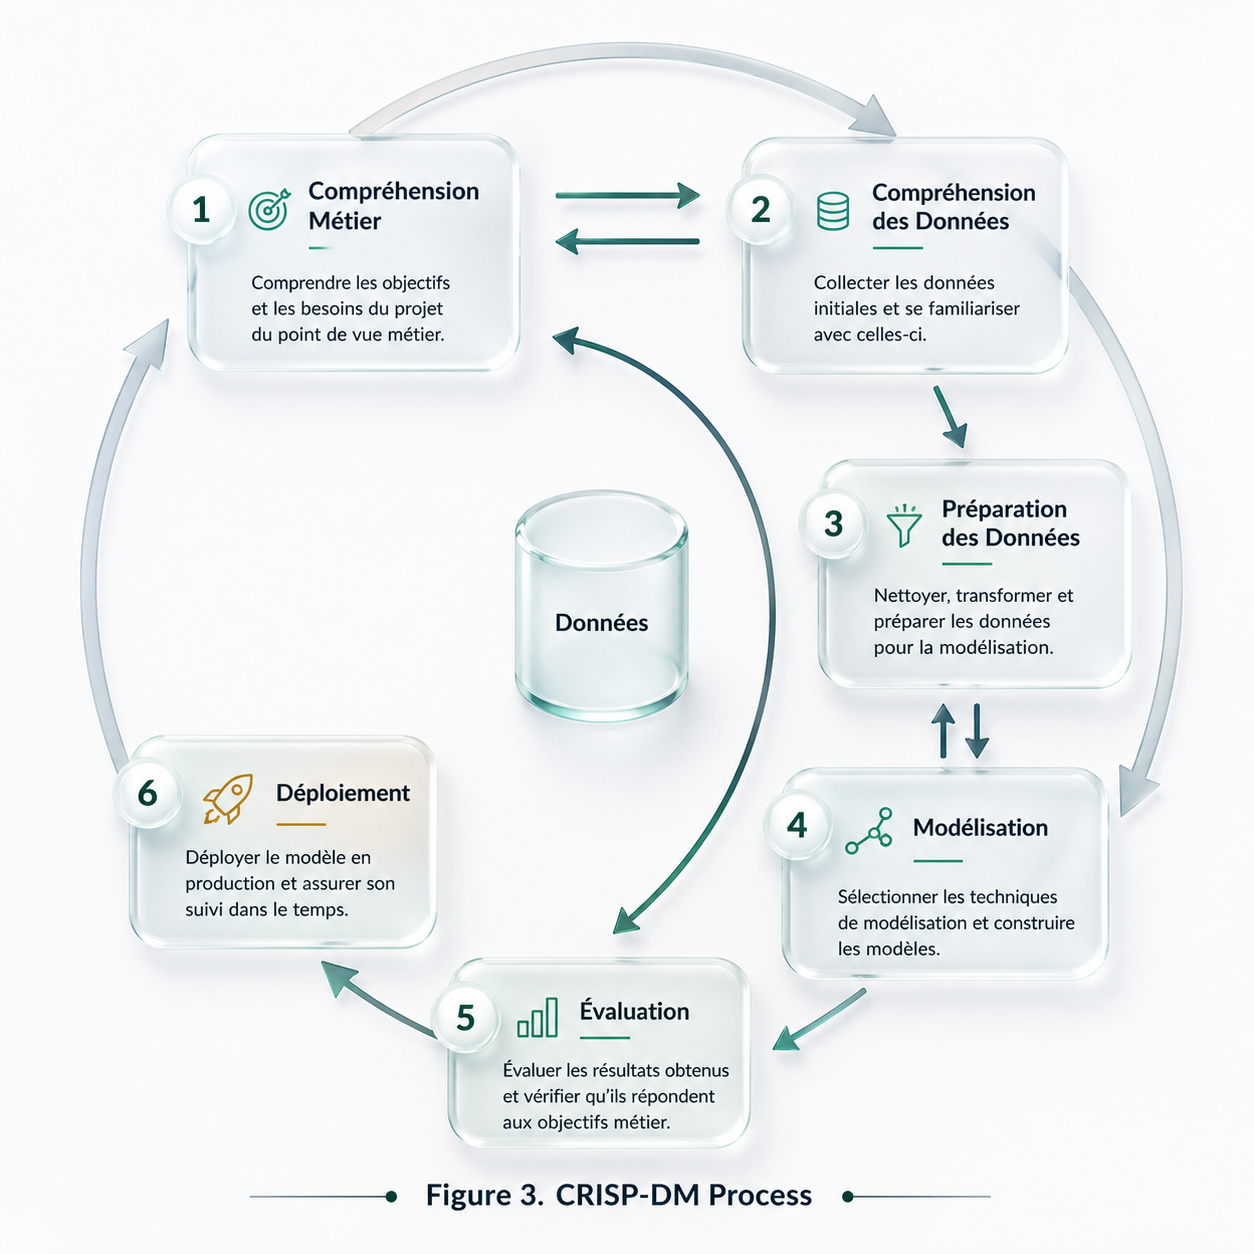
\includegraphics[width=0.6\linewidth]{crispDm.png}
    \caption{Processus CRISP-DM}
    \label{fig:crispdm}
\end{figure}


\section{Conclusion}
Ce chapitre a permis de présenter le contexte global du projet, ses enjeux ainsi que la problématique à résoudre. Il a également mis en évidence les objectifs visés et la méthodologie retenue pour structurer le travail. Le chapitre suivant sera consacré à l’analyse détaillée des besoins du système.

% ===== CHAPITRE 2 =====
\chapter{Analyse des besoins et spécification}

\section{Introduction}

Dans ce chapitre, nous passons de la compréhension du besoin métier à une description détaillée du système à réaliser. Cette étape est essentielle car elle permet de définir clairement les attentes, les fonctionnalités ainsi que les contraintes du système.

Nous allons d’abord analyser les solutions existantes afin d’identifier leurs limites, puis déterminer les acteurs du système. Ensuite, nous décrivons les besoins fonctionnels et non fonctionnels, avant de présenter les diagrammes de cas d’utilisation qui illustrent les interactions entre les utilisateurs et la plateforme.

Cette analyse constitue une base importante pour la phase de conception présentée dans le chapitre suivant.



\section{Identification des acteurs}

Dans notre système, le terme \textbf{Utilisateur} désigne tout acteur authentifié pouvant accéder à la plateforme. Il représente un acteur général regroupant les deux rôles principaux du système : \textbf{Agent} et \textbf{Administrateur}. Chaque utilisateur dispose de droits d’accès selon son rôle.

Les acteurs spécialisés sont les suivants :

\textbf{Agent :}  
L’agent utilise la plateforme pour gérer les réclamations des clients. Il est chargé de consulter les réclamations, de les analyser et de suivre leur traitement. Il peut également ajouter des notes internes, filtrer les réclamations selon différents critères et mettre à jour leur état (par exemple : en attente, en cours ou traitée).

\textbf{Administrateur :}  
L’administrateur est responsable de la gestion des utilisateurs. Il peut ajouter, modifier ou supprimer des comptes, ainsi que gérer leurs rôles.  
Il assure également le bon fonctionnement du système et peut classer manuellement les réclamations si nécessaire.

Ces deux acteurs accèdent à la plateforme via une interface sécurisée nécessitant une authentification.

\section{Besoins fonctionnels}

Les besoins fonctionnels décrivent les différentes fonctionnalités que le système doit offrir aux utilisateurs. Ils se résument comme suit :
\begin{itemize}

\item \textbf{Collecte des réclamations :}  
Le système doit permettre de récupérer automatiquement les réclamations à partir de différentes sources telles que les réseaux sociaux (Facebook, LinkedIn) .

\item \textbf{Extraction des données :}  
Le système doit extraire les informations importantes des réclamations, telles que le texte, l’auteur, la date et le lien de la réclamation.

\item \textbf{Stockage des données :}  
Les réclamations doivent être enregistrées dans une base de données avec leurs informations (texte, canal, date, catégorie, statut, etc.).

\item \textbf{Classification automatique :}  
Le système doit analyser le contenu des réclamations et les classer automatiquement selon leur catégorie à l’aide des techniques de NLP.

\item \textbf{Calcul du score d’urgence :}  
Le système doit attribuer un score d’urgence à chaque réclamation afin de faciliter la priorisation.

\item \textbf{Consultation des réclamations :}  
L’utilisateur doit pouvoir consulter la liste des réclamations avec leurs détails (texte, catégorie, canal, date, statut).

\item \textbf{Filtrage et recherche :}  
Le système doit permettre de filtrer les réclamations selon plusieurs critères (canal, catégorie, statut, score d'urgence ) et effectuer des recherches.

\item \textbf{Gestion des réclamations :}  
L’agent doit pouvoir :
\begin{itemize}
\item modifier le statut (par exemple : en attente, en cours ou traitée)
\item ajouter des notes internes
\item consulter les détails d’une réclamation
\end{itemize}

\item \textbf{Classification manuelle :}  
L’administrateur doit pouvoir classer manuellement les réclamations si nécessaire.

\item \textbf{Gestion des utilisateurs :}  
L’administrateur doit pouvoir ajouter, modifier et supprimer les comptes utilisateurs.

\item \textbf{Authentification :}  
Le système doit permettre aux utilisateurs de se connecter et se déconnecter de manière sécurisée.

\item \textbf{Tableau de bord (Dashboard) :}  
Le système doit proposer un tableau de bord interactif permettant de visualiser :
\begin{itemize}
\item le nombre total de réclamations
\item le nombre de réclamations en attente, en cours et traitées
\item la répartition des réclamations par catégorie
\item la répartition par canal (Facebook, LinkedIn)
\end{itemize}
\end{itemize}

\section{Besoins non fonctionnels}

Les besoins non fonctionnels définissent les contraintes et les qualités attendues du système. Ils peuvent être résumés comme suit :

\begin{itemize}

\item \textbf{Performance :}  
Le système doit être capable de traiter les réclamations dans un temps raisonnable et d’afficher les résultats rapidement.

\item \textbf{Sécurité :}  
L’accès à la plateforme doit être sécurisé à l’aide d’un système d’authentification. Les données des utilisateurs doivent être protégées contre les accès non autorisés.

\item \textbf{Fiabilité :}  
Le système doit garantir l’intégrité des données et assurer un fonctionnement stable sans perte d’information.

\item \textbf{Ergonomie :}  
L’interface utilisateur doit être simple, claire et facile à utiliser, afin de faciliter la navigation et l’utilisation des différentes fonctionnalités.

\item \textbf{Scalabilité :}  
Le système doit pouvoir gérer une augmentation du nombre de réclamations sans dégradation des performances.

\item \textbf{Maintenabilité :}  
Le code doit être structuré et bien organisé afin de faciliter les mises à jour et les évolutions futures.

\item \textbf{Disponibilité :}  
Le système doit être accessible à tout moment avec un minimum d’interruptions.

\item \textbf{Traçabilité :}  
Toutes les actions effectuées (modification de statut, ajout de note, etc.) doivent être enregistrées pour assurer le suivi des opérations.

\end{itemize}

\section{Diagramme de cas d’utilisation général}

Le diagramme de cas d’utilisation général (Figure~\ref{fig:diag_cu_general}) présente une vue d’ensemble des interactions entre les acteurs et le système. Il met en évidence les principales fonctionnalités accessibles ainsi que le rôle de chaque acteur.

\begin{figure}[H]
    \centering
    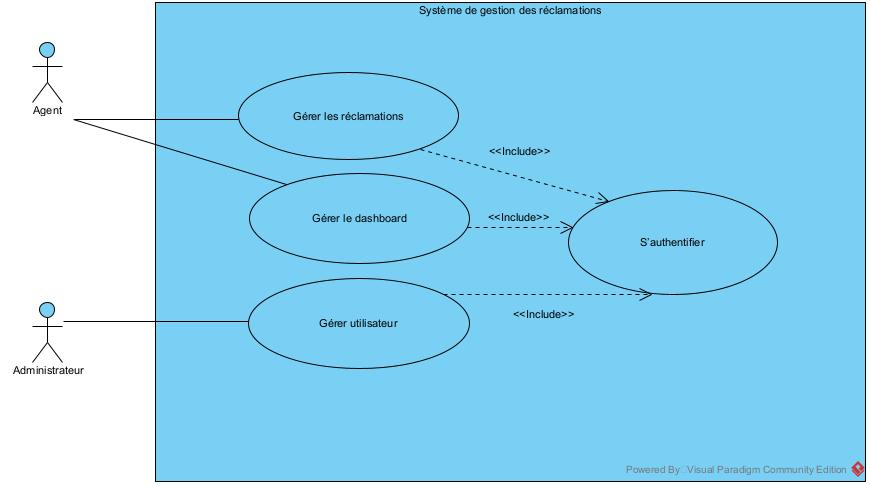
\includegraphics[width=0.8\textwidth]{use case global.jpg}
    \caption{Diagramme de cas d’utilisation général}
    \label{fig:diag_cu_general}
\end{figure}

\section{Diagramme de cas d’utilisation détaillé}

Le diagramme de cas d’utilisation détaillé (Figure~\ref{fig:diag_cu_detaille}) permet de représenter de manière précise les interactions entre les acteurs et les différentes fonctionnalités du système. Il met en évidence les scénarios principaux ainsi que les relations entre les cas d’utilisation.

\begin{figure}[H]
    \centering
    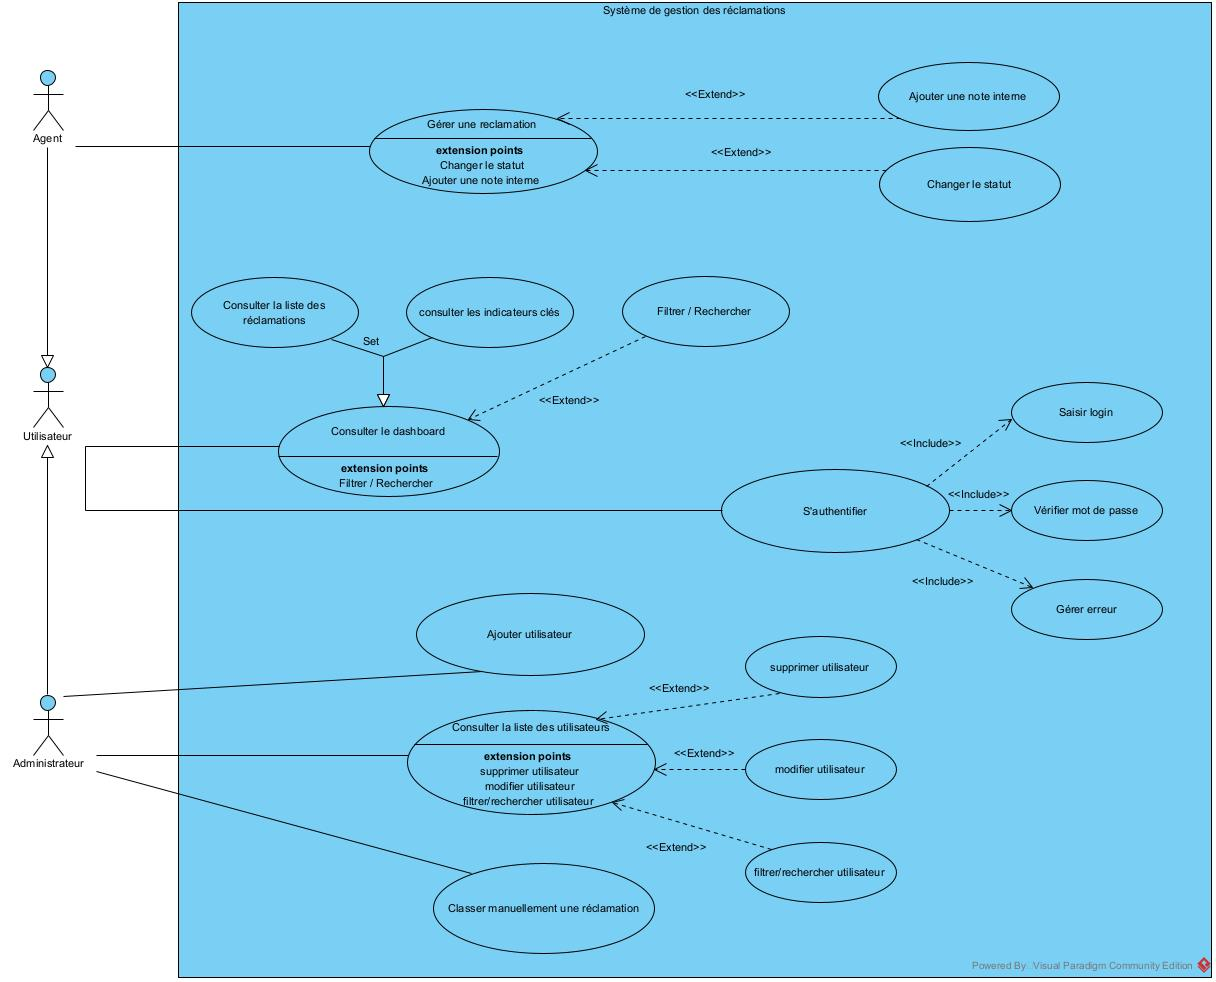
\includegraphics[width=0.8\textwidth]{cas d'utilisation detaillé.jpg}
    \caption{Diagramme de cas d’utilisation détaillé}
    \label{fig:diag_cu_detaille}
\end{figure}


\section{Fiches descriptives des cas d’utilisation}

Afin de mieux préciser le comportement attendu du système, les principaux cas d’utilisation sont décrits sous forme de fiches synthétiques.

\begin{table}[H]
\centering
\small
\caption{Fiche descriptive du cas d’utilisation : Authentification}
\begin{tabular}{|p{4cm}|p{9cm}|}
\hline
\textbf{Élément} & \textbf{Description} \\
\hline
Acteur & Utilisateur \\
\hline
Objectif & Permettre à un agent ou à un administrateur d’accéder à la plateforme de manière sécurisée. \\
\hline
Précondition & L’utilisateur possède un compte actif. \\
\hline
Scénario principal & L’utilisateur saisit son email et son mot de passe. Le système vérifie les informations saisies et autorise l’accès si elles sont valides. \\
\hline
Résultat attendu & L’utilisateur accède aux fonctionnalités autorisées selon son rôle. \\
\hline
\end{tabular}
\end{table}

\begin{table}[H]
\centering
\small
\caption{Fiche descriptive du cas d’utilisation : Consulter les réclamations}
\begin{tabular}{|p{4cm}|p{9cm}|}
\hline
\textbf{Élément} & \textbf{Description} \\
\hline
Acteur & Agent, Administrateur \\
\hline
Objectif & Permettre à l’utilisateur de consulter la liste des réclamations détectées par le système. \\
\hline
Précondition & L’utilisateur est authentifié. \\
\hline
Scénario principal & L’utilisateur accède à la page des réclamations. Le système affiche la liste des réclamations avec leurs informations principales : texte, source, catégorie, urgence et statut. \\
\hline
Résultat attendu & La liste des réclamations est affichée et peut être exploitée pour le suivi. \\
\hline
\end{tabular}
\end{table}

\begin{table}[H]
\centering
\small
\caption{Fiche descriptive du cas d’utilisation : Filtrer et rechercher une réclamation}
\begin{tabular}{|p{4cm}|p{9cm}|}
\hline
\textbf{Élément} & \textbf{Description} \\
\hline
Acteur & Agent, Administrateur \\
\hline
Objectif & Faciliter la recherche d’une réclamation selon des critères précis. \\
\hline
Précondition & L’utilisateur est authentifié et la liste des réclamations est disponible. \\
\hline
Scénario principal & L’utilisateur saisit un mot-clé ou sélectionne un filtre, par exemple la catégorie, la source, le statut ou le niveau d’urgence. Le système met à jour la liste selon les critères choisis. \\
\hline
Résultat attendu & Les réclamations correspondant aux critères de recherche sont affichées. \\
\hline
\end{tabular}
\end{table}

\begin{table}[H]
\centering
\small
\caption{Fiche descriptive du cas d’utilisation : Traiter une réclamation}
\begin{tabular}{|p{4cm}|p{9cm}|}
\hline
\textbf{Élément} & \textbf{Description} \\
\hline
Acteur & Agent \\
\hline
Objectif & Permettre à l’agent de suivre et traiter une réclamation client. \\
\hline
Précondition & L’agent est authentifié et la réclamation existe dans le système. \\
\hline
Scénario principal & L’agent consulte le détail d’une réclamation, ajoute une note interne si nécessaire, modifie son statut et marque la réclamation comme traitée après prise en charge. \\
\hline
Résultat attendu & La réclamation est mise à jour et l’action effectuée est enregistrée dans l’historique. \\
\hline
\end{tabular}
\end{table}

\begin{table}[H]
\centering
\small
\caption{Fiche descriptive du cas d’utilisation : Classifier manuellement une réclamation}
\begin{tabular}{|p{4cm}|p{9cm}|}
\hline
\textbf{Élément} & \textbf{Description} \\
\hline
Acteur & Administrateur \\
\hline
Objectif & Corriger ou compléter la classification d’une réclamation lorsque le système ne parvient pas à la classer avec une confiance suffisante. \\
\hline
Précondition & L’administrateur est authentifié et la réclamation est disponible. \\
\hline
Scénario principal & L’administrateur consulte la réclamation, analyse son contenu, choisit la catégorie appropriée et ajoute éventuellement une note administrative. \\
\hline
Résultat attendu & La catégorie de la réclamation est mise à jour et la correction manuelle est enregistrée. \\
\hline
\end{tabular}
\end{table}

\begin{table}[H]
\centering
\small
\caption{Fiche descriptive du cas d’utilisation : Gérer les utilisateurs}
\begin{tabular}{|p{4cm}|p{9cm}|}
\hline
\textbf{Élément} & \textbf{Description} \\
\hline
Acteur & Administrateur \\
\hline
Objectif & Permettre à l’administrateur de gérer les comptes des utilisateurs de la plateforme. \\
\hline
Précondition & L’administrateur est authentifié. \\
\hline
Scénario principal & L’administrateur consulte la liste des utilisateurs, ajoute un nouvel utilisateur, modifie ses informations ou désactive un compte existant. \\
\hline
Résultat attendu & Les informations des utilisateurs sont mises à jour dans la base de données. \\
\hline
\end{tabular}
\end{table}

\section{Conclusion}

Dans ce chapitre, nous avons analysé les besoins du système et identifié les principales fonctionnalités attendues. Cette étape nous a permis de mieux comprendre les exigences du projet et constitue une base essentielle pour la phase de conception, qui sera présentée dans le chapitre suivant.
% ===== CHAPITRE 3 =====
\chapter{Conception de la solution}

\section{Introduction}

Après l’analyse des besoins, cette étape consiste à concevoir la solution à mettre en place. Elle permet de définir l’architecture du système ainsi que les différents composants qui le constituent.

Dans ce chapitre, nous présentons l’architecture globale de la plateforme, les diagrammes UML, la conception de la base de données, les API ainsi que le module de traitement intelligent basé sur le NLP.

Cette étape est essentielle car elle permet de structurer le système avant sa phase de développement.

\section{Environnement technique}

La réalisation de la solution s’appuie sur plusieurs outils et technologies, utilisés pour la conception, le développement backend, le développement frontend, la gestion de la base de données et le traitement intelligent des réclamations.

\begin{itemize}
    \item \textbf{Visual Paradigm :} outil utilisé pour la modélisation UML, notamment les diagrammes de cas d’utilisation, le diagramme de classes et les diagrammes de séquence.

    \begin{figure}[H]
        \centering
        
\includegraphics[width=0.25\linewidth]{logo.png}
        \caption{Logo de Visual Paradigm}
    \end{figure}

    \item \textbf{Django REST Framework :} framework utilisé pour développer les API backend et gérer les échanges entre le frontend, la base de données et les modules métier \cite{drf}.

    \begin{figure}[H]
        \centering
        
\includegraphics[width=0.25\linewidth]{django.png}
        \caption{Logo de Django}
    \end{figure}

    \item \textbf{React :} bibliothèque JavaScript utilisée pour développer l’interface web de la plateforme \cite{react}.

    \begin{figure}
        \centering
        
\includegraphics[width=0.25\linewidth]{logo4.png}
        \caption{Logo de React}
    \end{figure}

    \item \textbf{PostgreSQL :} système de gestion de base de données utilisé pour stocker les commentaires, les annotations NLP, les réclamations, les utilisateurs et l’historique des actions \cite{postgresql}.

    \begin{figure}[H]
        \centering
        
\includegraphics[width=0.25\linewidth]{logo1.png}
        \caption{Logo de PostgreSQL}
    \end{figure}

    \item \textbf{FastAPI :} framework utilisé pour exposer le module NLP sous forme d’API de prédiction \cite{fastapi}.

    \begin{figure}[H]
        \centering
        
\includegraphics[width=0.25\linewidth]{logo2.png}
        \caption{Logo de FastAPI}
    \end{figure}

    \item \textbf{Python :} langage utilisé pour le développement du backend, des scripts de collecte, du prétraitement et du module NLP.

    \begin{figure}[H]
        \centering
        
\includegraphics[width=0.25\linewidth]{logo5.png}
        \caption{Logo de python}
    \end{figure}

    \item \textbf{Scikit-learn :} bibliothèque utilisée pour la vectorisation TF-IDF et l’entraînement des modèles de Machine Learning \cite{scikitlearn}.

    \begin{figure}[H]
        \centering
        
\includegraphics[width=0.25\linewidth]{logo3.png}
        \caption{Logo de Scikit-learn}
    \end{figure}

    \item \textbf{Ollama / Mistral :} outils utilisés pour intégrer un modèle de langage dans l’approche hybride ML + LLM.

    \begin{figure}[H]
    \centering

    \begin{minipage}{0.45\textwidth}
        \centering
        \caption{Ollama, utilisé pour l’exécution locale du LLM}
    \end{minipage}
    \hfill
    \begin{minipage}{0.45\textwidth}
        \centering
        \caption{Mistral, modèle de langage utilisé}
    \end{minipage}

\end{figure}

    \item \textbf{Playwright :} outil utilisé pour automatiser la collecte de données à partir de pages web dynamiques.

    \begin{figure}[H]
        \centering
        
\includegraphics[width=0.25\linewidth]{logo.png}
        \caption{Outil de collecte automatisée utilisé dans le projet}
    \end{figure}
    
\end{itemize}

\section{Architecture globale du système}

L’architecture du système repose sur une organisation en plusieurs couches permettant de séparer les différentes fonctionnalités de la plateforme et d’assurer une meilleure modularité.

Le système est composé de plusieurs composants principaux :

\begin{itemize}

\item \textbf{Interface Web et Tableau de bord BI :}  
Ils représentent l’interface utilisateur développée avec React. Cette interface permet à l’agent et à l’administrateur d’interagir avec la plateforme, de consulter et traiter les réclamations, d’accéder aux indicateurs, aux statistiques et aux graphiques du tableau de bord.


\item \textbf{Backend Django :}  
Il constitue le cœur applicatif du système. Il est développé avec Django et Django REST Framework. Il reçoit les requêtes HTTP/JSON provenant de l’interface web, gère les utilisateurs, les réclamations et les opérations métier, puis communique avec la base de données pour lire ou modifier les informations nécessaires.


\item \textbf{Base de données :}  
Elle stocke les informations du système, notamment les utilisateurs, les commentaires, les réclamations, les statuts, les annotations et les actions effectuées. Elle échange avec le backend via des opérations SQL/CRUD et fournit également les textes nécessaires au module NLP.

\item \textbf{API NLP FastAPI :}  
Ce composant est séparé du backend principal. Il assure le prétraitement du texte, la vectorisation TF-IDF, l’utilisation des modèles ML, l’intégration du LLM Mistral/Ollama, du LLM-as-a-Judge et l’application des règles métier afin de produire le résultat final de l’analyse.

\end{itemize}

Les différents composants communiquent entre eux à travers des requêtes HTTP au format JSON et des échanges SQL avec la base de données. Cette organisation permet de séparer l’interface utilisateur, le backend applicatif, le stockage des données et le module NLP, ce qui améliore la maintenabilité, la modularité et l’évolutivité de la plateforme.


\begin{figure}[H]
    \centering
    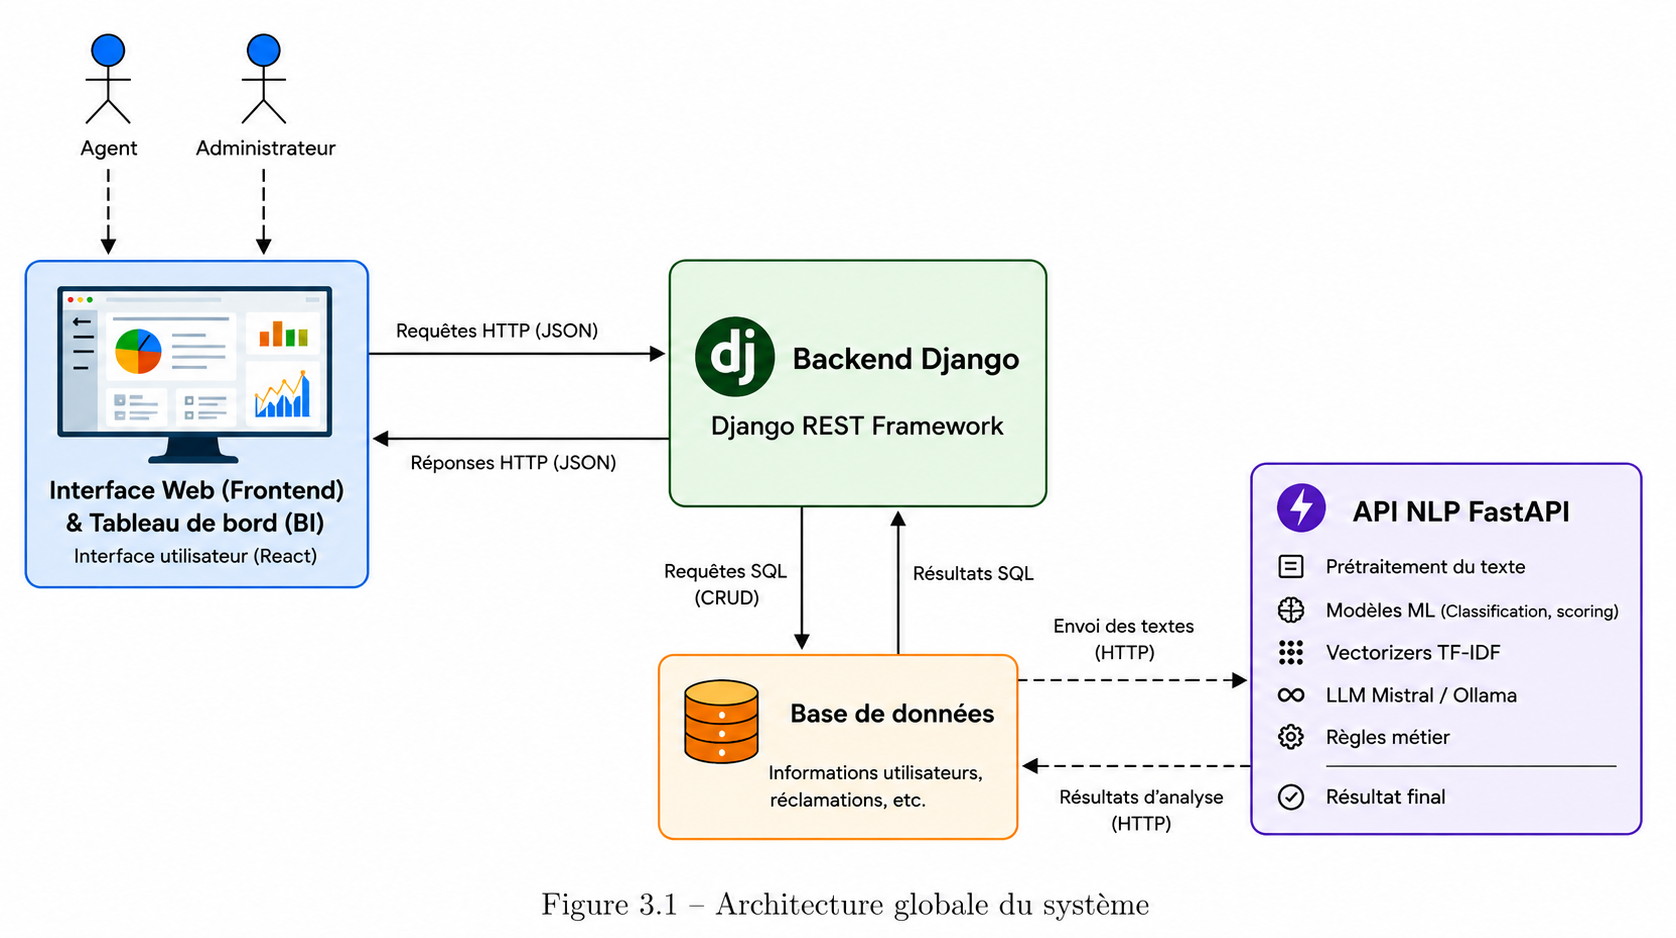
\includegraphics[width=1\linewidth]{architecture du systeme.png}
    \caption{Architecture globale du système}
\end{figure}

\section{Diagrammes UML}
Avant de présenter les différents diagrammes, il est important de préciser que la modélisation du système a été réalisée en utilisant le langage UML (Unified Modeling Language). UML est un langage standard largement utilisé pour la conception et la modélisation des systèmes informatiques. Il permet de représenter de manière claire et structurée les différents aspects d’un système, qu’ils soient statiques ou dynamiques.

Dans ce projet, plusieurs types de diagrammes UML ont été utilisés, notamment le diagramme de classes pour représenter la structure du système, ainsi que les diagrammes de séquence pour illustrer le déroulement des interactions entre les différents composants.

Pour la réalisation de ces diagrammes, l’outil Visual Paradigm a été utilisé. Cet outil offre un environnement complet pour la conception UML, permettant de créer des diagrammes professionnels, lisibles et conformes aux standards. Il facilite également l’organisation et la mise à jour des modèles tout au long du projet.
Dans cette phase de conception, les diagrammes UML ont été utilisés afin de modéliser le système de manière claire et structurée.

Les diagrammes de cas d’utilisation, présentés dans le chapitre précédent, ont permis d’identifier les principales fonctionnalités du système ainsi que les interactions entre les acteurs et la plateforme.

Dans ce chapitre, nous nous intéressons principalement au diagramme de classes et aux diagrammes de séquence.

\subsection{Diagramme de classes}

Le diagramme de classes (Figure~\ref{fig:diag_classe}) représente la structure statique du système. Il met en évidence les principales classes, leurs attributs, leurs méthodes ainsi que les relations entre elles. Le Tableau~\ref{tab:classes_systeme} présente une description synthétique des classes utilisées dans notre système.

\begin{figure}[H]
    \centering
    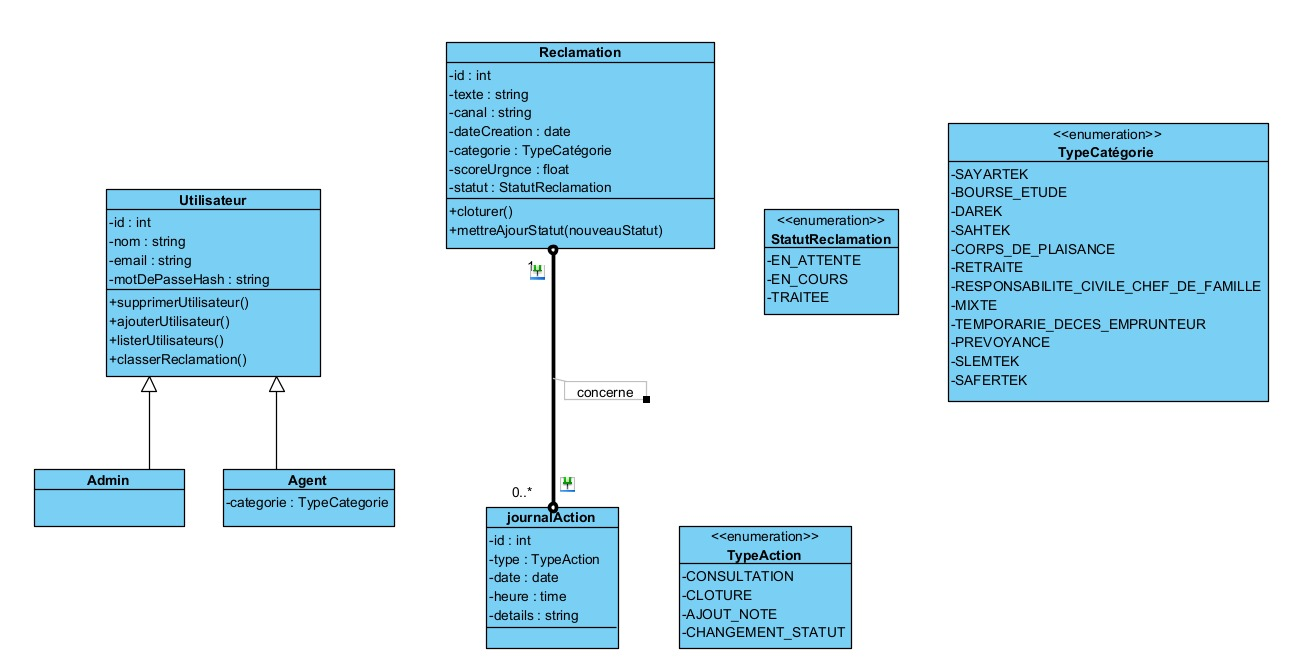
\includegraphics[width=1\linewidth]{diag_classe.png}
    \caption{Diagramme de classes du système}
    \label{fig:diag_classe}
\end{figure}

Dans l’implémentation, les agents et les administrateurs sont stockés dans une même table \textbf{Utilisateur}. Le champ \texttt{role} permet de distinguer leurs droits d’accès. Dans le diagramme UML, les classes \textbf{Agent} et \textbf{Admin} sont représentées comme des spécialisations de la classe \textbf{Utilisateur} afin de montrer les fonctionnalités propres à chaque rôle.


\begin{table}[H]
\centering
\small
\caption{Description des principales classes du système}
\label{tab:classes_systeme}
\begin{tabular}{|p{3.5cm}|p{9cm}|}
\hline
\textbf{Classe} & \textbf{Description} \\
\hline
Utilisateur & Représente les utilisateurs du système. Elle contient les informations principales comme l’identifiant, le nom, l’email, le mot de passe haché, le rôle, la catégorie assignée et l’état du compte. \\
\hline
Agent & Représente un utilisateur chargé de consulter, filtrer et traiter les réclamations. Il peut être associé à une catégorie selon son domaine de traitement. \\
\hline
Admin & Représente l’administrateur du système. Il peut gérer les utilisateurs et classifier manuellement certaines réclamations si nécessaire. \\
\hline
Commentaire & Représente un commentaire collecté depuis une source numérique. Il contient le texte original, le texte nettoyé, la source, l’auteur, la date du commentaire et l’URL associée. \\
\hline
Annotation & Représente le résultat du traitement NLP appliqué à un commentaire. Elle contient l’indication permettant de savoir si le commentaire est une réclamation, la catégorie prédite, le niveau d’urgence, le statut de traitement ainsi que les informations liées à une éventuelle correction manuelle. \\
\hline
Réclamation & Représente le cas de réclamation créé lorsqu’un commentaire est identifié comme une réclamation. Elle contient les informations de suivi, notamment le statut, l’agent assigné, la date d’ouverture, la date de traitement et la note interne. \\
\hline
JournalAction & Permet d’enregistrer les actions effectuées sur les réclamations, comme l’ajout d’une note, le changement de statut, la clôture ou toute autre action de suivi. \\
\hline
StatutRéclamation & Énumération qui définit les différents états possibles d’une réclamation : en attente, en cours ou traitée. \\
\hline
TypeCatégorie & Énumération qui représente les catégories possibles des réclamations, comme sinistre auto, sinistre IRDS, sinistre vie ou service client. \\
\hline
\end{tabular}
\end{table}

Ce tableau permet de mieux comprendre le rôle de chaque classe dans le système. La classe \textbf{Commentaire} représente la donnée collectée, tandis que la classe \textbf{Annotation} contient le résultat de l’analyse NLP. Lorsqu’un commentaire est identifié comme une réclamation, un cas de \textbf{Réclamation} est créé afin d’assurer son suivi. La classe \textbf{JournalAction} permet quant à elle de conserver l’historique des opérations effectuées sur chaque réclamation.


\subsection{Diagrammes de séquence}

Les diagrammes de séquence (Figures~\ref{fig:seq_liste} à \ref{fig:seq_collecte}) illustrent le déroulement des interactions entre les différents composants du système. Ils permettent de représenter de manière dynamique les échanges entre l’interface utilisateur, le backend API, le module NLP et la base de données. Le Tableau~\ref{tab:seq} présente une synthèse des principaux scénarios modélisés.

\begin{figure}[H]
    \centering
    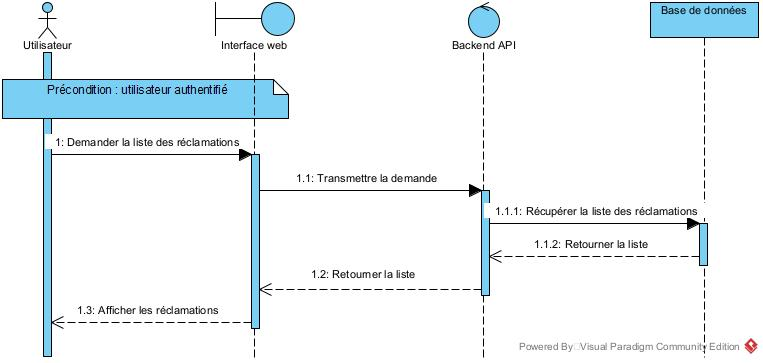
\includegraphics[width=0.9\textwidth]{consultation de la liste des réclamations.jpeg}
    \caption{Diagramme de séquence : consultation de la liste des réclamations}
    \label{fig:seq_liste}
\end{figure}

\begin{figure}[H]
    \centering
    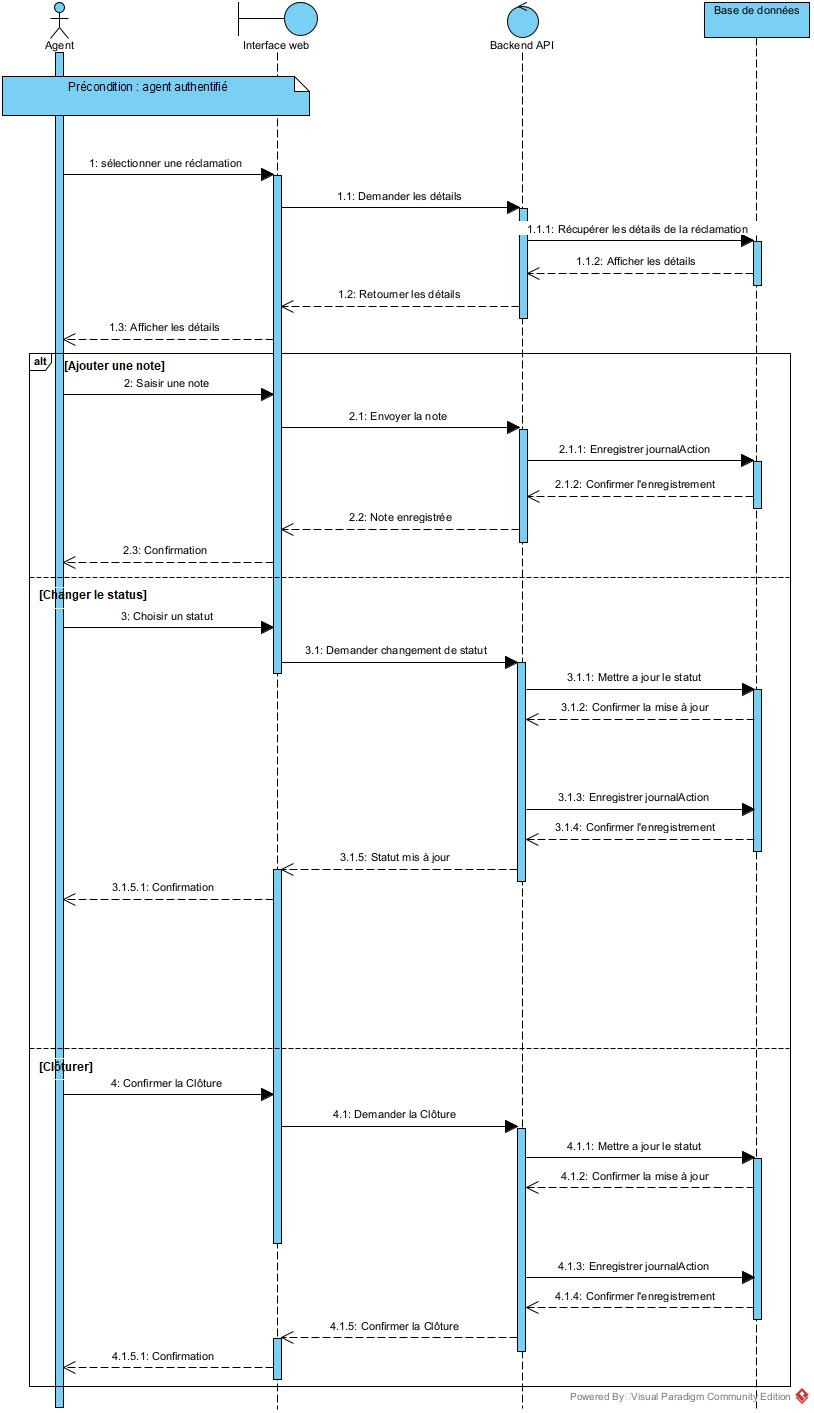
\includegraphics[width=0.8\textwidth]{Diagramme_de_séquence_traitement_d’une_réclamation.jpeg}
    \caption{Diagramme de séquence : traitement d’une réclamation}
    \label{fig:seq_traitement}
\end{figure}



\begin{figure}[H]
    \centering
    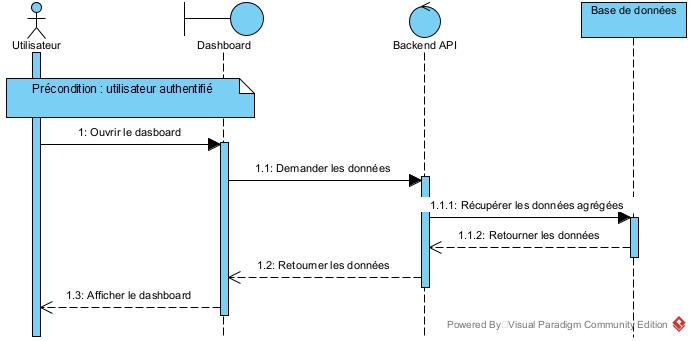
\includegraphics[width=0.9\textwidth]{affichage du dashboard.jpeg}
    \caption{Diagramme de séquence : affichage du dashboard}
    \label{fig:seq_dashboard}
\end{figure}

\begin{figure}[H]
    \centering
    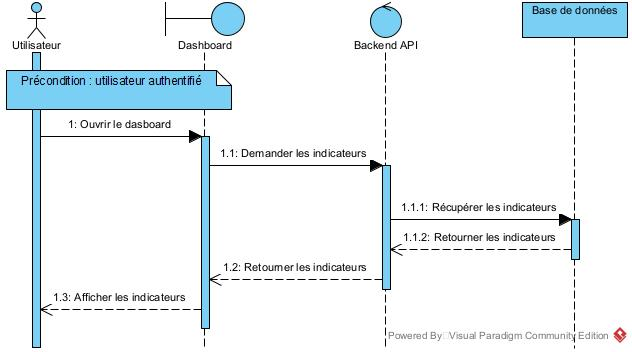
\includegraphics[width=0.9\textwidth]{consultation des indicateurs du dashboard.jpeg}
    \caption{Diagramme de séquence : consultation des indicateurs du dashboard}
    \label{fig:seq_indicateurs}
\end{figure}

\begin{figure}[H]
    \centering
    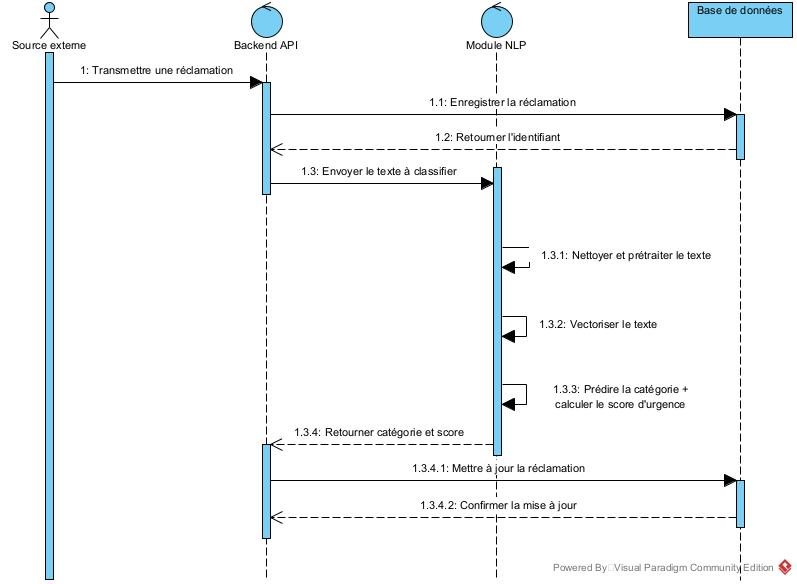
\includegraphics[width=0.9\textwidth]{classification automatique des réclamations via le module NLP.jpeg}
    \caption{Diagramme de séquence : classification automatique des réclamations via le module NLP}
    \label{fig:seq_nlp}
\end{figure}

\begin{figure}[H]
    \centering
    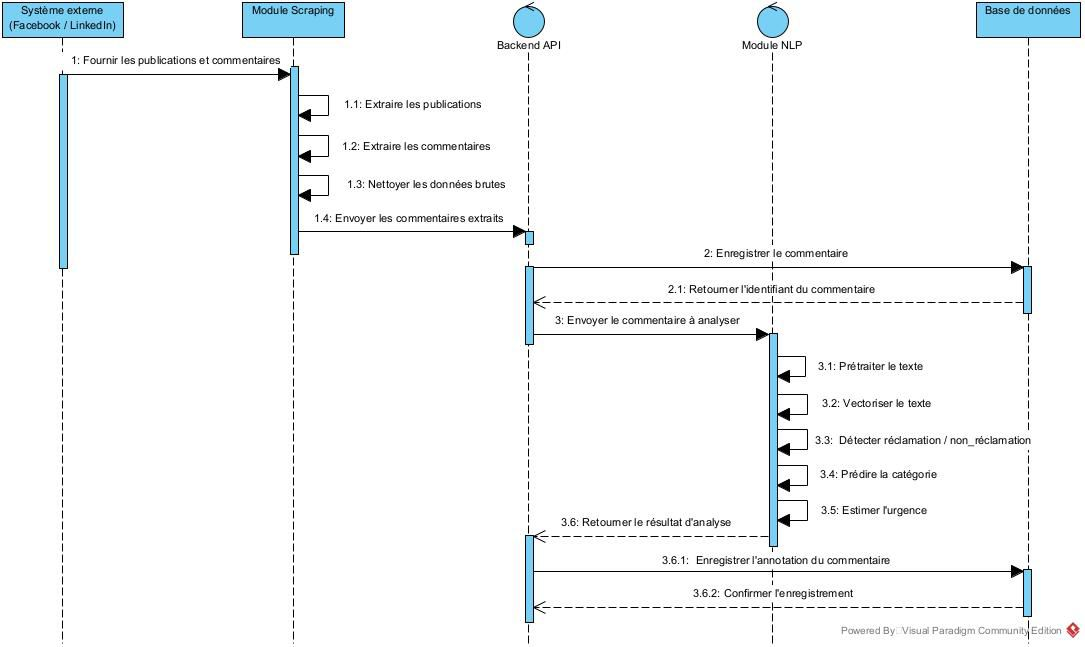
\includegraphics[width=0.9\textwidth]{collecte et traitement intelligent des réclamations.jpeg}
    \caption{Diagramme de séquence : collecte et traitement intelligent des réclamations}
    \label{fig:seq_collecte}
\end{figure}

\begin{table}[H]
\centering
\small
\caption{Description des scénarios des diagrammes de séquence}
\label{tab:seq}
\begin{tabular}{|p{4cm}|p{9cm}|}
\hline
\textbf{Scénario} & \textbf{Description} \\
\hline
Consultation des réclamations & Permet à l’utilisateur de consulter la liste des réclamations via l’interface. \\
\hline
Traitement d’une réclamation & Permet à l’agent de gérer une réclamation en ajoutant des notes, en modifiant le statut ou en la clôturant. \\
\hline
Filtrage des réclamations & Permet de rechercher et filtrer les réclamations selon des critères spécifiques. \\
\hline
Affichage du dashboard & Permet de visualiser les données globales du système. \\
\hline
Consultation des indicateurs & Permet d’afficher les indicateurs clés. \\
\hline
Classification automatique (NLP) & Permet d’analyser les réclamations pour déterminer leur catégorie et leur urgence. \\
\hline
Collecte et traitement & Permet de collecter et traiter automatiquement les données provenant de sources externes. \\
\hline
\end{tabular}
\end{table}

Ce tableau met en évidence les différents scénarios d’interaction ainsi que le rôle des composants dans le fonctionnement dynamique du système.
\FloatBarrier

\section{Conception de la base de données}

La base de données joue un rôle essentiel dans notre système, car elle permet de stocker et d’organiser toutes les informations nécessaires au bon fonctionnement de la plateforme.

Dans notre projet, la conception de la base de données s’appuie sur le diagramme de classes présenté précédemment. Elle regroupe les principales entités du système, notamment les utilisateurs, les réclamations ainsi que les différentes actions réalisées sur celles-ci.

La table \textbf{Utilisateur} contient les informations relatives aux comptes des utilisateurs, telles que l’identifiant, le nom, l’adresse email et le mot de passe. Elle permet de gérer les différents profils du système, en particulier l’agent et l’administrateur.

La table \textbf{Réclamation} constitue l’élément central de la base de données. Elle regroupe les informations essentielles liées aux réclamations, comme le texte, le canal, la date de création, la catégorie, le score d’urgence ainsi que le statut. Ces informations permettent d’assurer le suivi et le traitement des réclamations.

La table \textbf{JournalAction} permet d’enregistrer les différentes opérations réalisées sur les réclamations. Elle assure la traçabilité des actions effectuées, telles que la consultation, le changement de statut, l’ajout d’une note interne ou la clôture d’une réclamation.

En complément, certaines données sont représentées sous forme d’énumérations, comme le type de catégorie, le statut de la réclamation et le type d’action. Cela permet de mieux organiser les données et de limiter les valeurs possibles à des choix prédéfinis.

Le schéma relationnel suivant présente les principales tables utilisées dans la base de données ainsi que leurs relations.

\begin{table}[H]
\centering
\small
\caption{Schéma relationnel simplifié de la base de données}
\begin{tabular}{|p{3.5cm}|p{5cm}|p{5cm}|}
\hline
\textbf{Table} & \textbf{Champs principaux} & \textbf{Relations} \\
\hline
\texttt{app\_users} & id, name, email, password, role, assigned\_category, is\_active & Utilisée pour identifier les agents et les administrateurs. \\
\hline
\texttt{comments} & id, source, author\_name, comment\_date, url, text\_original, clean\_text & Un commentaire peut être associé à une annotation et à une réclamation. \\
\hline
\texttt{annotations} & id, comment\_id, is\_reclamation, category, urgency, processing\_status, admin\_note & Relation One-to-One avec \texttt{comments} via \texttt{comment\_id}. \\
\hline
\texttt{reclamation\_cases} & id, comment\_id, status, assigned\_agent, opened\_at, processed\_at, internal\_note & Relation One-to-One avec \texttt{comments} via \texttt{comment\_id}. \\
\hline
\texttt{reclamation\_action\_logs} & id, case\_id, actor\_name, actor\_role, action, details, created\_at & Relation Many-to-One avec \texttt{reclamation\_cases} via \texttt{case\_id}. \\
\hline
\end{tabular}
\end{table}

Cette conception permet d’obtenir une base de données cohérente, bien structurée et adaptée aux besoins du système. Elle facilite également l’exploitation des données par les différentes composantes de l’application, notamment le backend, le module NLP et le dashboard.
\section{Conception des API}
Dans notre système, les API (Application Programming Interface) jouent un rôle essentiel dans la communication entre les différentes composantes de la plateforme, notamment le frontend, le backend, la base de données et le module NLP.

\begin{itemize}
    \item \textbf{Objectif des API :}
\end{itemize}
\vspace{0.3cm}
Les API permettent de :

\begin{enumerate}
    \item recevoir les données issues du processus de scraping (Facebook et LinkedIn) 
    \item traiter les données selon la logique métier
    \item interagir avec la base de données PostgreSQL
    \item exploiter le module NLP pour analyser les commentaires
    \item retourner les résultats sous format JSON
\end{enumerate}

\begin{itemize}
    \item \textbf{Architecture des API :}
\end{itemize}
\vspace{0.3cm}
Le backend principal du système est implémenté à l’aide de Django et Django REST Framework. Il permet de gérer les routes, les vues API, la sérialisation des données et la communication avec l’interface web. En complément, une API NLP basée sur FastAPI est utilisée comme composant séparé pour exécuter la prédiction intelligente des commentaires \cite{drf,fastapi}.

L’architecture des API repose sur une approche modulaire, assurant la communication entre les différents composants du système. Les API jouent un rôle central dans l’orchestration des opérations de traitement, notamment en assurant l’interaction entre le module de collecte, le module NLP et la base de données.

Dans ce cadre, une API de prédiction a été conçue pour permettre l’analyse automatique des commentaires. Cette API agit comme un point d’accès au module NLP et permet de déclencher le processus de classification.

Lorsqu’une donnée est transmise à l’API, celle-ci appelle une fonction interne de traitement qui applique une logique de décision basée sur une approche hybride combinant des modèles de Machine Learning et un modèle de langage (LLM).

Le résultat produit est ensuite structuré et renvoyé sous un format standardisé, facilitant son exploitation par les autres composants du système.
\clearpage

\begin{itemize}
    \item \textbf{Logique de traitement :}
\end{itemize}
\vspace{0.3cm}
Lorsqu’une requête est envoyée :
\begin{itemize}
    \item le texte est reçu par l’API.
    \item le texte est transmis au module interne de traitement.
    \item le modèle ML produit une première prédiction avec un score de confiance.
    \item si la confiance est suffisante, le résultat ML est validé.
    \item si la confiance est insuffisante, le système appelle le LLM Mistral via Ollama.
    \item si le résultat du LLM reste incertain ou non classé, le LLM-as-a-Judge vérifie la cohérence de la prédiction.
    \item si l’incertitude persiste, une intervention humaine peut être effectuée.
    \item le résultat final est retourné au client au format JSON.
\end{itemize}


\vspace{0.3cm}
\begin{itemize}
    \item \textbf{Intégration avec la base de données :}
\end{itemize}
\vspace{0.3cm}
Les résultats de l’API sont exploités dans un script de traitement automatique chargé d’assurer la persistance des données dans la base PostgreSQL.

Ce processus comprend les étapes suivantes :

\begin{enumerate}
    \item récupération des commentaires non encore analysés depuis la base de données .
    \item envoi de ces commentaires au module de prédiction via l’API .
    \item réception des résultats d’analyse (réclamation, catégorie, urgence) .
    \item enregistrement des résultats dans la table annotations .
    \item création d’une entrée dans la table \(reclamation_cases\) pour les commentaires identifiés comme réclamations.
\end{enumerate}

Ce mécanisme permet d’assurer une mise à jour continue de la base de données et de garantir la traçabilité des analyses effectuées.

\begin{itemize}
    \item \textbf{Intégration dans le pipeline global :}
\end{itemize}
\vspace{0.3cm}
Les API s’intègrent dans un pipeline global de traitement des données permettant d’automatiser l’ensemble du processus, depuis la collecte jusqu’à l’analyse.

Ce pipeline comprend les étapes suivantes :

\begin{enumerate}
    \item \textbf{Scraping des données :} collecte automatique des publications et commentaires depuis les plateformes Facebook et LinkedIn .
    \item \textbf{Extraction des commentaires :} identification et structuration des données textuelles pertinentes .
    \item \textbf{Nettoyage :} prétraitement des textes afin d’éliminer le bruit et standardiser les données .
    \item \textbf{Chargement en base de données :} stockage des commentaires nettoyés dans PostgreSQL .
    \item \textbf{Classification via API :} analyse automatique des commentaires à l’aide du module NLP pour déterminer leur nature, leur catégorie et leur niveau d’urgence.
\end{enumerate}

Ce pipeline est exécuté de manière automatisée, garantissant un traitement continu et cohérent des données collectées.

\begin{itemize}
    \item \textbf{Avantages de cette conception :}
\end{itemize}
\vspace{0.3cm}
Cette conception présente plusieurs avantages :

\begin{enumerate}
    \item \textbf{Modularité du système :} chaque composant (scraping, API, NLP, base de données) fonctionne de manière indépendante, ce qui facilite la maintenance et l’évolution du système .
    \item \textbf{Séparation claire des responsabilités :} chaque module assure une fonction spécifique (collecte, traitement, analyse), ce qui améliore la lisibilité et l’organisation globale du système .
    \item \textbf{Possibilité d’évolution :} l’architecture basée sur les API permet d’ajouter facilement de nouvelles fonctionnalités ou d’intégrer de nouveaux services sans modifier l’ensemble du système .
    \item \textbf{Facilité d’intégration :} l’utilisation d’API et du format JSON permet une intégration simple avec d’autres applications ou systèmes externes.
\end{enumerate}

\section{Conception du module NLP}
Le module NLP constitue le cœur intelligent du système. Il permet d’analyser automatiquement les commentaires clients afin de détecter les réclamations, les classifier et estimer leur niveau d’urgence.

\begin{itemize}
    \item \textbf{Objectifs du module :}
\end{itemize}
\vspace{0.3cm}
Le module NLP vise à automatiser l’analyse des commentaires en remplissant les fonctions suivantes :

\begin{enumerate}
    \item \textbf{Détection des réclamations :} identifier automatiquement si un commentaire constitue une réclamation ou non .
    \item \textbf{Classification des réclamations :} attribuer une catégorie pertinente aux réclamations détectées .
    \item \textbf{Estimation de l’urgence :} évaluer le niveau de priorité du traitement (faible, moyenne ou élevée).
\end{enumerate}

Ces objectifs permettent d’améliorer la gestion des interactions clients et d’optimiser la prise de décision.

\begin{itemize}
    \item \textbf{Architecture du module :}
\end{itemize}
\vspace{0.3cm}
Le module NLP repose sur une approche hybride combinant :

\begin{enumerate}
    \item des \textbf{modèles de Machine Learning (ML)}, qui constituent une branche de l’intelligence artificielle permettant aux systèmes d’apprendre à partir des données et de réaliser des prédictions, pour le traitement rapide et efficace des cas simples.
    \item un \textbf{modèle de langage (LLM – Large Language Model)}, qui est un modèle avancé d’intelligence artificielle capable de comprendre et de générer du texte en langage naturel grâce à un apprentissage sur de grandes quantités de données, pour traiter les cas complexes ou ambigus nécessitant une meilleure compréhension contextuelle \cite{ibmllm,hftransformers}.
    \item un \textbf{mécanisme LLM-as-a-Judge}, utilisé lorsque le résultat du LLM reste incertain, afin de valider la cohérence de la prédiction avant son affichage \cite{ibmeval}.

\end{enumerate}

Cette combinaison permet d’obtenir un bon compromis entre performance, rapidité et précision.

\begin{itemize}
    \item \textbf{Étapes de traitement :}
\end{itemize}
\vspace{0.3cm}
\begin{enumerate}
    \item \textbf{Extraction des commentaires}



Les données sont collectées depuis les plateformes Facebook et LinkedIn sous forme de fichiers JSON. Cette étape consiste à extraire les commentaires et à structurer les informations (texte, date, auteur,  source,url).

    \item \textbf{Prétraitement du texte}

Les commentaires extraits contiennent souvent du bruit. Un prétraitement est donc appliqué afin d’améliorer la qualité des données. Il comprend :

\begin{itemize}
    \item suppression des emails et des URLs .
    \item suppression des hashtags .
    \item suppression de la ponctuation et des caractères spéciaux .
    \item normalisation du texte (mise en minuscules, suppression des espaces inutiles).
\end{itemize}

Cette étape permet de rendre les données exploitables par les modèles d’apprentissage automatique.

    \item \textbf{Vectorisation}

Après nettoyage, les textes sont transformés en représentations numériques à l’aide de la méthode TF-IDF (Term Frequency - Inverse Document Frequency).

Cette technique permet de :

\begin{itemize}
    \item représenter les mots sous forme de vecteurs .
    \item attribuer un poids aux termes en fonction de leur importance .
    \item réduire l’impact des mots peu informatifs.
\end{itemize}

La vectorisation est essentielle pour permettre aux modèles de Machine Learning de traiter les données textuelles.

    \item \textbf{Modélisation Machine Learning}

Le système utilise trois modèles de classification basés sur l’algorithme Logistic Regression \cite{logreg} :

\begin{enumerate}
    \item un modèle de détection des réclamations .
    \item un modèle de classification des catégories .
    \item un modèle d’estimation de l’urgence.
\end{enumerate}

Ces modèles sont entraînés à partir d’un jeu de données annoté et permettent d’obtenir des prédictions rapides et efficaces.

    \item \textbf{Approche hybride ML + LLM} 

Afin d’améliorer la précision du module NLP, le système adopte une stratégie hybride combinant un modèle de Machine Learning et un modèle de langage. Dans un premier temps, le modèle ML analyse le commentaire et retourne une prédiction accompagnée d’un score de confiance.

Lorsque le score de confiance du modèle ML est \textbf{supérieur ou égal} au seuil défini, le résultat est directement validé et utilisé par le système. En revanche, lorsque ce score est \textbf{insuffisant}, le système fait appel au modèle de langage LLM afin d’effectuer une analyse plus approfondie du commentaire.

Le LLM permet de mieux comprendre le contexte, les nuances linguistiques et les cas ambigus. Il propose alors une prédiction complémentaire, comprenant le type du commentaire, la catégorie et le niveau d’urgence.


    \item \textbf{Validation par LLM-as-a-Judge}

Après la prédiction initiale du modèle ML, le système conserve les scores de confiance associés, notamment le score lié à la détection de réclamation et celui lié à la classification de la catégorie. Lorsque le modèle ML présente une confiance insuffisante, le système peut faire appel au LLM afin d’obtenir une analyse contextuelle complémentaire du commentaire.

Même lorsque la prédiction finale est proposée par le LLM, les scores de confiance du modèle ML restent utilisés comme indicateurs d’incertitude. Ainsi, si le LLM est appelé parce que le modèle ML était peu confiant, notamment au niveau de la catégorie, le système peut déclencher le mécanisme LLM-as-a-Judge.

Le LLM-as-a-Judge peut également intervenir lorsque la prédiction finale est directement proposée par le modèle ML, mais que ses scores de confiance restent insuffisants. Dans ce cas, il agit comme une étape de vérification supplémentaire afin d’éviter de valider automatiquement une prédiction incertaine.

Il peut aussi intervenir lorsque la catégorie obtenue est \texttt{non\_classée}, ce qui signifie que le système a détecté une réclamation sans pouvoir l’associer de manière fiable à une catégorie précise. Il peut également être déclenché lorsque le niveau d’urgence est élevé, car ce type de cas nécessite une validation supplémentaire avant d’être priorisé dans le système.

Le rôle du LLM-as-a-Judge est alors de vérifier la cohérence entre le commentaire original et la prédiction proposée par le système, qu’elle provienne du ML ou du LLM. Il peut soit valider cette prédiction, soit proposer une correction avant son enregistrement.


\end{enumerate}

\vspace{0.3cm}
\begin{itemize}
    \item \textbf{Logique de décision :}
\end{itemize}
\vspace{0.3cm}
\textbf{Logique de décision}

La décision finale repose sur un mécanisme basé sur des seuils de confiance
issus des prédictions du modèle de Machine Learning.

Trois cas sont distingués :

\begin{itemize}
    \item Si le score de confiance du modèle ML est \textbf{supérieur ou égal au seuil}, le résultat ML est directement validé.
    \item Si le score ML est \textbf{inférieur au seuil}, le système fait appel au LLM afin d’obtenir une analyse complémentaire.
    \item Si la prédiction reste sensible ou incertaine, par exemple en cas de catégorie \texttt{non\_classée}, de confiance ML faible ou d’urgence élevée, le mécanisme LLM-as-a-Judge intervient pour valider ou corriger le résultat.
\end{itemize}


Cette approche permet de combiner la rapidité du Machine Learning avec la précision du modèle LLM.

\begin{figure}[H]
    \centering
    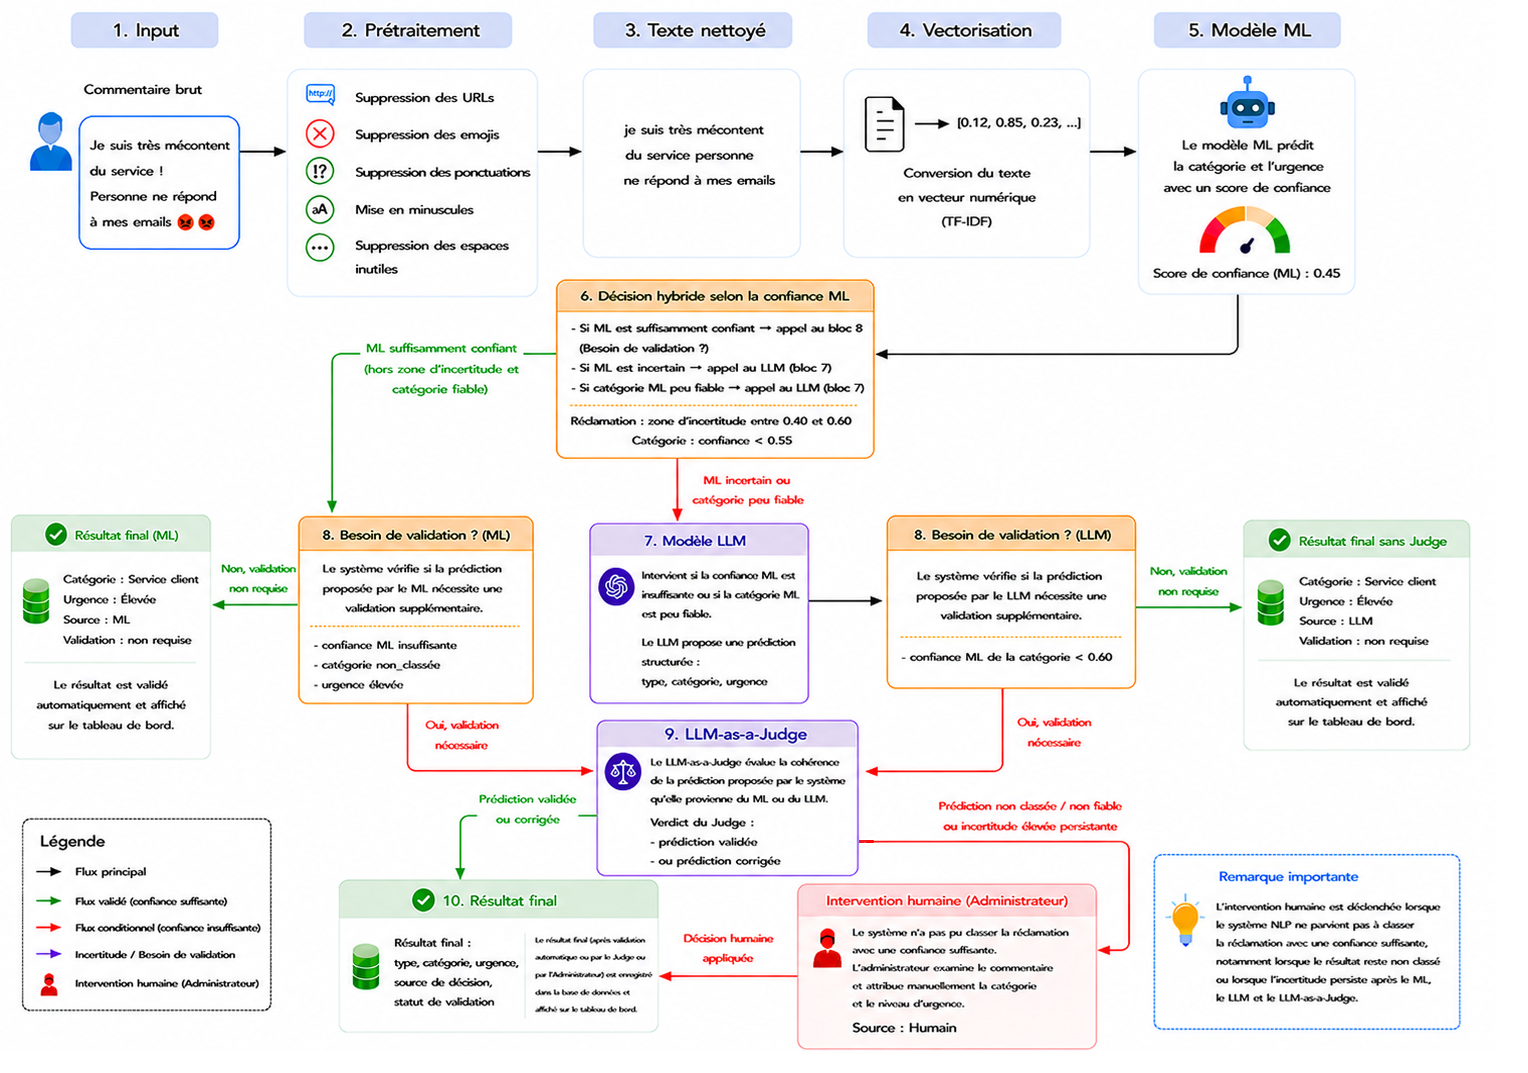
\includegraphics[width=1\linewidth]{Untitled.png}
    \caption{Fonctionnement du module NLP}
\end{figure}

Cette figure illustre le processus complet de traitement des commentaires au sein du module NLP. Après le prétraitement et la vectorisation TF-IDF, le texte est analysé par un modèle de Machine Learning qui prédit le type, la catégorie et le niveau d’urgence avec un score de confiance. Si ce score est supérieur au seuil défini, le résultat du modèle ML est directement validé et enregistré. Dans le cas contraire, le système fait appel à un modèle de langage (LLM) afin d’affiner l’analyse. Si la prédiction nécessite une validation supplémentaire, notamment en cas de faible confiance ML, de catégorie \texttt{non\_classée} ou d’urgence élevée, le LLM-as-a-Judge intervient comme mécanisme de validation final afin d’évaluer la cohérence, la pertinence et la fiabilité du résultat avant son enregistrement et son affichage.



\begin{itemize}
    \item \textbf{Résultat du module NLP :}
\end{itemize}
\vspace{0.3cm}
    Le module retourne un objet structuré contenant :
    \begin{itemize}
            \item le type de commentaire (réclamation ou non) .
            \item la catégorie associée
            \item le niveau d’urgence
            \item le score de confiance final
            \item la source de la prédiction, indiquée par le champ \texttt{source} : \texttt{ml} ou \texttt{llm}
            \item le statut de validation, indiqué par le champ \texttt{processing\_status} : \texttt{no\_judge}, \texttt{validated\_by\_judge} ou \texttt{corrected\_by\_judge}


    \end{itemize}
    Ces résultats sont ensuite :
    \begin{itemize}
            \item stockés dans la base de données pour assurer la traçabilité .
            \item utilisés pour le suivi des réclamations .
            \item exploités dans le dashboard pour l’analyse et la visualisation.
    \end{itemize}

\begin{itemize}
    \item \textbf{Avantages du module NLP :}
\end{itemize}
\vspace{0.3cm}
Le module NLP présente plusieurs avantages :

\begin{enumerate}
    \item automatisation du traitement des commentaires : réduction de l’intervention humaine .
    \item amélioration de la précision grâce à l’approche hybride ML + LLM .
    \item gain de temps dans l’analyse des données ;
    \item meilleure priorisation des réclamations en fonction de leur urgence.
\end{enumerate}

\begin{itemize}
    \item \textbf{Intervention humaine et validation des résultats :}


    Malgré l’automatisation offerte par le module NLP, une intervention humaine reste possible afin d’assurer la fiabilité des résultats.
    
    En effet, un administrateur peut :
    
    \begin{itemize}
        \item corriger la classification d’une réclamation mal identifiée .
        \item attribuer manuellement une catégorie à un commentaire lorsque l’IA ne parvient pas à le classifier correctement .
    \end{itemize}
\end{itemize}
Cette approche permet de combiner l’efficacité de l’intelligence artificielle avec l’expertise humaine, garantissant ainsi une meilleure qualité des résultats.

\section{Conclusion}
Ce chapitre a présenté la conception générale de la plateforme, en mettant en évidence son architecture, son modèle de données, ses API et son module NLP. Ces éléments serviront de base pour l’implémentation technique décrite dans les chapitres suivants.

% ===== CHAPITRE 4 =====
\chapter{Collecte et préparation des données}

\section{Introduction}
La qualité des résultats d’un système intelligent dépend directement de la qualité des données utilisées. Dans ce projet, les réclamations clients constituent une source d’information essentielle, mais elles sont généralement non structurées et nécessitent un traitement préalable.

Ce chapitre présente les sources de données, les méthodes de collecte ainsi que les étapes de préparation appliquées afin de rendre ces données exploitables par le module NLP.

\section{Sources de données}
Dans notre projet, les données utilisées sont principalement des commentaires clients collectés à partir de réseaux sociaux, notamment Facebook et LinkedIn. Ces plateformes constituent des espaces où les utilisateurs expriment leurs avis, leurs demandes d’information ainsi que leurs réclamations concernant les services proposés.

Les principales sources de données sont :

\begin{itemize}
    \item \textbf{Facebook :} les commentaires ont été collectés à partir de publications liées à la MAE, où les utilisateurs expriment leurs expériences, leurs remarques et leurs réclamations.
    \item \textbf{LinkedIn :} certaines publications et interactions ont également été exploitées afin d’enrichir la base de commentaires et de diversifier les sources de données.
\end{itemize}

Ces données se présentent sous forme de texte libre, ce qui signifie qu’elles ne suivent pas une structure fixe. Elles peuvent contenir des erreurs, des abréviations, des emojis, des caractères spéciaux ou des formulations en plusieurs langues, ce qui rend leur traitement plus complexe.



\section{Méthodes de collecte}
Dans le cadre de la collecte automatique des données, nous avons recours à une technique appelée \textbf{web scraping}, qui correspond à un procédé d’extraction automatisée de données issues du web. Il permet d’extraire des données non structurées, puis de les transformer en un format exploitable pour l’analyse. Cette technique est particulièrement utilisée pour collecter de grandes quantités de données à partir de différentes plateformes en ligne, notamment les réseaux sociaux.

\vspace{0.3cm}

Dans ce projet, la collecte des données a été réalisée de manière automatique à l’aide de scripts développés en \textbf{Python} et \textbf{JavaScript}, en s’appuyant principalement sur la bibliothèque \textbf{Playwright} pour simuler la navigation sur les plateformes sociales.

\begin{itemize}
    \item \textbf{Collecte des données Facebook}
\end{itemize}
Pour Facebook, une approche basée sur l’automatisation du navigateur a été utilisée. Le script ouvre la page cible, simule le défilement (scroll) afin de charger les publications dynamiquement, puis extrait les informations des posts.

Le processus comprend :
\begin{enumerate}
    \item navigation vers la page Facebook ciblée .
    \item détection des publications visibles dans le DOM .
    \item extraction des liens des posts .
    \item récupération des informations principales .
    \item extraction des commentaires et des réponses associées.
\end{enumerate}
Le script utilise des techniques avancées comme :
\begin{enumerate}
    \item le défilement progressif pour charger plus de contenu.
    \item l’interaction avec les boutons.
    \item l’analyse du HTML pour identifier les données pertinentes.
\end{enumerate}
Ces opérations sont automatisées à l’aide de Playwright, permettant une collecte dynamique et robuste des données.

\begin{itemize}
    \item \textbf{Collecte des données LinkedIn}
\end{itemize}
Pour LinkedIn, un scraper spécifique a été développé afin d’extraire les publications d’une entreprise ainsi que leurs commentaires.

Le processus est le suivant :

\begin{enumerate}
    \item accès à la page LinkedIn de l’entreprise .
    \item extraction des publications à l’aide d’un scraper personnalisé .
    \item navigation vers chaque publication .
    \item extraction des commentaires, auteurs et dates.
    \item conversion des dates relatives en format standard.
\end{enumerate}
Les données extraites incluent :

\begin{enumerate}
    \item le texte du post .
    \item la date de publication .
    \item le nombre de commentaires .
    \item les commentaires détaillés (auteur, texte, date).
\end{enumerate}

Le scraping est réalisé à l’aide d’un gestionnaire de navigateur et d’un module dédié à l’extraction des posts



\section{Description des données}
Les données collectées sont structurées sous forme d’objets représentant les publications et leurs commentaires.

\begin{enumerate}
    \item \textbf{Structure des données}

    Chaque publication contient les éléments suivants :
    
    \begin{itemize}
        \item URL du post
        \item Identifiant du post
        \item Auteur
        \item Contenu textuel (caption)
        \item Date de publication
        \item Nombre de commentaires
        \item Nombre de partages (Facebook)
        \item Liste des commentaires
    \end{itemize}
    Chaque commentaire est décrit par :
    \begin{itemize}
        \item Auteur
        \item Texte
        \item Date du commentaire
        \item Lien du commentaire
        \item Réponses (replies)
    \end{itemize}
    Cette structure est définie à l’aide de modèles de données permettant d’organiser les informations extraites.
    
    \item \textbf{Nature des données}
    
    Les données collectées présentent les caractéristiques suivantes :
    
    \begin{itemize}
        \item données textuelles non structurées
        \item présence de bruit (caractères spéciaux, emojis, répétitions)
        \item formats de dates hétérogènes
        \item structure imbriquée (commentaires + réponses)
    \end{itemize}
\end{enumerate}

Ces caractéristiques rendent nécessaire un traitement approfondi avant exploitation.

\section{Nettoyage et prétraitement des données}
Afin de rendre les données exploitables, plusieurs étapes de nettoyage et de transformation ont été appliquées.

\begin{enumerate}
    \item \textbf{Nettoyage du texte}


    Les textes extraits contiennent souvent du bruit. Les opérations suivantes ont été appliquées :
    
    \begin{itemize}
        \item conversion en minuscules 
        \item suppression des emails
        \item suppression des URLs
        \item suppression des hashtags
        \item suppression de la ponctuation
        \item suppression des symboles spéciaux
        \item suppression des espaces multiples
    \end{itemize}
    
    Le code inclut des fonctions spécifiques pour nettoyer et normaliser les contenus textuels.
    
        \item \textbf{Filtrage des commentaires}
    
    Tous les commentaires extraits ne sont pas pertinents. Un filtrage a été effectué pour :
    
    \begin{itemize}
        \item supprimer les commentaires vides
        \item ignorer les éléments non textuels (réactions, labels)
        \item conserver uniquement les commentaires avec auteur et contenu
    \end{itemize}
    
        \item \textbf{Normalisation des dates}
    
    Les dates récupérées sont souvent sous forme relative. Une fonction de transformation a été utilisée pour :
    
    \begin{itemize}
        \item convertir ces dates en format standard (jj/mm/aaaa)
        \item assurer l’uniformité des données.
    \end{itemize}
    
    Cette étape est essentielle pour permettre l’analyse temporelle des réclamations.
    
        \item \textbf{Structuration des données}
    
    Les données ont été transformées en objets structurés:
    
    \begin{itemize}
        \item conversion en format JSON
        \item organisation hiérarchique (post → commentaires → réponses)
        \item uniformisation des champs
    \end{itemize}
    
    Cette structuration facilite leur stockage et leur exploitation future.
\end{enumerate}

\section{Stockage initial}
Après traitement, les données sont stockées dans un format structuré afin de permettre leur utilisation dans les différentes composantes du système.

\begin{enumerate}
    \item \textbf{Format de stockage}

    Les données sont sauvegardées sous forme de fichiers JSON, contenant :
    
    \begin{itemize}
        \item les métadonnées de la collecte
        \item la liste des publications
        \item les commentaires associés
    \end{itemize}
    
    Ce format permet :
    
    \begin{itemize}
        \item une lecture facile
        \item une compatibilité avec les outils de traitement NLP
        \item une intégration simple avec le backend
    \end{itemize}

    Après le stockage intermédiaire en JSON, les commentaires nettoyés sont chargés dans la base de données PostgreSQL afin d’être exploités par le backend et le module NLP.


     \item \textbf{Organisation des données}
    
    Les données sont organisées de manière hiérarchique :
    
    \begin{itemize}
            \item niveau 1 : publications
            \item niveau 2 : commentaires
            \item niveau 3 : réponses aux commentaires
    \end{itemize}
    
    Cette organisation permet de conserver la structure réelle des interactions entre utilisateurs.
    
     \item \textbf{Exploitation future}
    
    Les données stockées sont ensuite utilisées pour :
    
    \begin{itemize}
        \item la classification des réclamations
        \item le calcul du score d’urgence
        \item l’analyse statistique
        \item l’alimentation du dashboard
    \end{itemize}
\end{enumerate}


\section{Conclusion}
Dans ce chapitre, nous avons présenté le processus de collecte et de préparation des données. Les traitements appliqués permettent d’obtenir des données plus propres et exploitables pour les étapes ultérieures de développement et de modélisation.

% ===== CHAPITRE 5 =====
\chapter{Développement backend et base de données}

\section{Introduction}
Ce chapitre décrit l’implémentation de la partie backend de la plateforme. Il présente l’environnement technique, l’architecture adoptée, la gestion des réclamations, les API développées ainsi que la structure de la base de données.

\section{Environnement technique backend}

Le développement du backend de la plateforme repose principalement sur le langage \textbf{Python} et le framework \textbf{Django}. Django a été choisi pour sa robustesse, sa structure claire et les fonctionnalités qu’il propose pour le développement d’applications web sécurisées et maintenables.

Afin d’exposer les fonctionnalités de la plateforme sous forme de services web, nous avons utilisé \textbf{Django REST Framework}. Ce framework permet de créer des API REST, de sérialiser les données, de gérer les requêtes HTTP et de faciliter la communication avec l’interface frontend développée avec React.

La base de données utilisée est \textbf{PostgreSQL}. Elle permet de stocker les utilisateurs, les commentaires collectés, les annotations produites par le module NLP, les réclamations détectées ainsi que l’historique des actions effectuées sur chaque réclamation.

L’accès aux données est assuré à travers le \textbf{Django ORM}, qui permet de manipuler les tables de la base sous forme d’objets Python. Cette approche facilite la gestion des relations entre les données, améliore la lisibilité du code et simplifie les opérations de création, lecture, modification et suppression.

Enfin, le backend intègre des mécanismes liés à l’authentification, aux permissions et à la sécurisation des échanges, notamment à travers l’utilisation de JWT et la configuration CORS pendant le développement.

\section{Architecture backend}
La figure ci-dessous présente l’architecture du backend de la plateforme. Cette architecture est organisée en plusieurs couches afin de séparer les responsabilités et de faciliter la maintenance du système.

\textbf{L’interface web} communique avec le backend à travers des requêtes HTTP au format JSON. Ces requêtes sont reçues par la couche API, développée avec Django REST Framework. Cette couche regroupe les routes, les vues API, les serializers, la validation des données, la gestion des erreurs, la pagination, le filtrage et les permissions.

La couche \textbf{Service} représente la logique métier de l’application. Elle assure la gestion des utilisateurs, la gestion des réclamations, le traitement des données, l’intégration du module NLP, l’application des règles métier ainsi que la journalisation des actions.

La couche \textbf{Data Access} repose sur le \textbf{Django ORM}. Elle permet de manipuler les modèles Django, d’effectuer les requêtes vers la base de données, de gérer les relations, les contraintes et les migrations.

Les données sont stockées dans une base \textbf{PostgreSQL} contenant les utilisateurs, les commentaires, les annotations, les réclamations et l’historique des actions.

La \textbf{sécurité} est représentée comme une couche transversale. Elle intervient à plusieurs niveaux du backend à travers l’authentification JWT, l’autorisation selon les rôles, la validation des données, la protection des routes, CORS, le hachage des mots de passe et la journalisation.

\textit{L’authentification JWT (JSON Web Token) est un mécanisme d’authentification basé sur l’utilisation de jetons numériques. Lorsqu’un utilisateur se connecte avec des identifiants valides, le backend génère un token qui contient certaines informations sur l’utilisateur, comme son identifiant, son email ou son rôle. Ce token est ensuite envoyé au frontend, qui l’utilise pour accéder aux routes protégées sans devoir renvoyer le mot de passe à chaque requête.}

\textit{CORS (Cross-Origin Resource Sharing) est un mécanisme utilisé afin d’autoriser la communication entre l’interface web React et le backend Django, qui peuvent fonctionner sur des adresses ou des ports différents durant le développement.}

\begin{figure}[H]
    \centering
    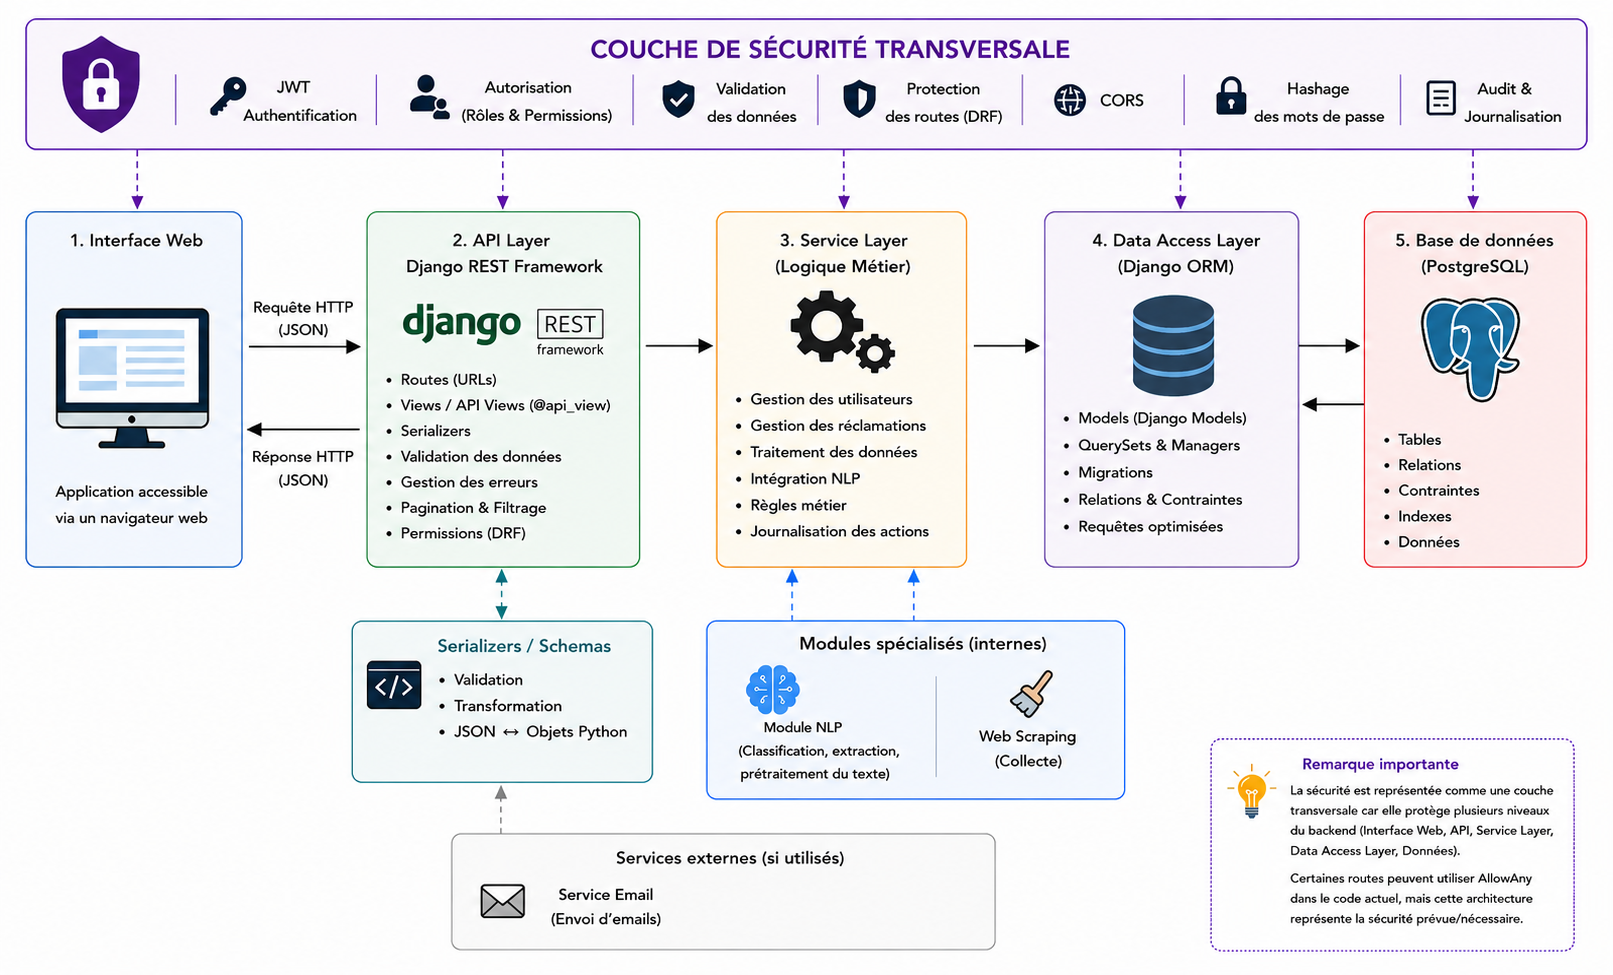
\includegraphics[width=1\linewidth]{architecture_backend.png}
    \caption{Architecture backend de la plateforme}
\end{figure}

\section{Conception et implémentation des API}
Les API jouent un rôle central dans le système en assurant la communication entre le frontend et le backend. Elles permettent de traiter les requêtes des utilisateurs et de retourner les résultats sous forme de données structurées.

\begin{itemize}
    \item \textbf{Types d’API développées}
\end{itemize}

Plusieurs types d’API ont été implémentés afin de couvrir les différentes fonctionnalités du système :

\begin{enumerate}
    \item \textbf{API d’authentification :} permettent aux utilisateurs de se connecter à la plateforme, de changer leur mot de passe et de demander une réinitialisation en cas d’oubli.
    \item \textbf{API des utilisateurs :}permettent à l’administrateur de consulter la liste des comptes, de créer de nouveaux utilisateurs, de modifier leurs informations et de supprimer les comptes qui ne sont plus nécessaires.
    \item \textbf{API des réclamations :} permettent de consulter la liste des réclamations, d’afficher les détails d’une réclamation, de mettre à jour son statut, d’ajouter des notes internes ou administratives, de classifier manuellement une réclamation et de récupérer des statistiques utiles au suivi.
\end{enumerate}

\begin{itemize}
    \item \textbf{Fonctionnalités principales}
\end{itemize}

Les API développées permettent de couvrir l’ensemble des besoins fonctionnels du système. Elles assurent notamment la consultation des réclamations, leur mise à jour ainsi que le suivi de leur état tout au long de leur cycle de traitement.

Elles offrent également la possibilité de modifier le statut des réclamations et d’ajouter des notes internes afin d’améliorer le suivi et la traçabilité des actions effectuées.

Par ailleurs, ces API permettent la gestion des utilisateurs et de leurs rôles, garantissant ainsi un contrôle d’accès adapté aux différents profils du système.

\begin{itemize}
    \item \textbf{Format des échanges}
\end{itemize}

Les données sont échangées au format JSON, ce qui facilite leur traitement, leur transmission et leur intégration avec l’interface web.

\section{Gestion des réclamations}
La gestion des réclamations constitue la fonctionnalité centrale du système.

\begin{itemize}
    \item \textbf{Cycle de vie d’une réclamation}

    \begin{enumerate}
        \item Collecte (scraping réseaux sociaux)
        \item Stockage initial
        \item Analyse NLP
        \item Classification
        \item Traitement par agent
        \item Clôture
    \end{enumerate}

\end{itemize}

\begin{itemize}
    \item \textbf{États d’une réclamation}
    \begin{itemize}
        \item en attente
        \item en cours
        \item traitée
    \end{itemize}
\end{itemize}

\begin{itemize}
    \item \textbf{Actions disponibles}

    Un agent peut :
    
    \begin{enumerate}
        \item consulter les réclamations
        \item modifier le statut
        \item ajouter des notes internes
        \item filtrer les données
    \end{enumerate}
\end{itemize}

\begin{itemize}
    \item \textbf{Traçabilité}

    Chaque action est enregistrée dans la table ReclamationActionLog afin d’assurer :
    
    \begin{itemize}
        \item le suivi des opérations
        \item l’historique des modifications
        \item la transparence
    \end{itemize}
    
    Chaque action effectuée sur une réclamation est enregistrée dans la table ReclamationActionLog afin de conserver l’historique des opérations : prise en charge, changement de statut, ajout de note, validation de catégorie ou clôture du traitement.

\end{itemize}

\section{Implémentation de la base de données}
La base de données est implémentée avec PostgreSQL et repose sur plusieurs tables principales.

\begin{itemize}
    \item \textbf{\texttt{app\_users} :} stocke les utilisateurs, leurs rôles, leurs emails, leur mot de passe haché, leur statut actif et leur catégorie assignée.
    \item \textbf{\texttt{comments} :} stocke les commentaires collectés, avec la source, l’auteur, la date, l’URL, le texte original et le texte nettoyé.
    \item \textbf{\texttt{annotations} :} stocke les résultats d’analyse NLP, notamment le type du commentaire, la catégorie, le niveau d’urgence, le statut de traitement et les informations de correction manuelle.
    \item \textbf{\texttt{reclamation\_cases} :} représente les réclamations détectées et suivies dans la plateforme. Elle contient le statut, l’agent assigné, la date d’ouverture, la date de traitement et les notes internes.
    \item \textbf{\texttt{reclamation\_action\_logs} :} conserve l’historique des actions effectuées sur chaque réclamation.

\end{itemize}

Les relations entre les tables permettent :

\begin{itemize}
    \item de lier les utilisateurs aux actions
    \item de suivre l’historique des réclamations
    \item d’assurer la traçabilité
\end{itemize}

\section{Gestion des utilisateurs}
Le système distingue deux types d’utilisateurs :
\begin{itemize}
\item\textbf{Agent}

    \begin{itemize}
        \item gère les réclamations
        \item consulte les données
        \item met à jour les statuts
    \end{itemize}
\item\textbf{Administrateur}
    \begin{itemize}
        \item gère les comptes utilisateurs
        \item contrôle le système
    \end{itemize}

\end{itemize}

\textbf{Authentification}

L’accès au système est sécurisé par JWT \cite{jwtio} :

\begin{itemize}
    \item génération d’un token après une connexion valide.
    \item stockage du token côté frontend pendant la session utilisateur.
    \item vérification du token lors de l’accès aux routes protégées.
    \item identification du rôle de l’utilisateur afin d’adapter les permissions.
\end{itemize}

\textbf{Autorisation}

Un système de rôles (RBAC) est utilisé pour limiter l’accès :

\begin{itemize}
    \item admin → accès complet
    \item agent → accès limité
\end{itemize}

Cela garantit la sécurité et la confidentialité des données.

\vspace{0.3cm}

Dans le cadre de cette version académique, certaines configurations d’accès ont été assouplies afin de faciliter les tests et la validation fonctionnelle de l’application. Pour un déploiement en environnement réel, ces routes devront être strictement protégées par JWT, par un contrôle des rôles et par des permissions adaptées à chaque type d’utilisateur.



\section{Conclusion}
Ce chapitre a permis de présenter le développement du backend et la mise en place de la base de données. Nous avons décrit les technologies utilisées, l’architecture adoptée, les API développées ainsi que les principales fonctionnalités implémentées.

Cette étape a permis de traduire les besoins fonctionnels en solutions techniques concrètes, assurant ainsi le bon fonctionnement de la plateforme.

% ===== CHAPITRE 6 =====
\chapter{Développement frontend et sécurité de l’application}
\section{Introduction}

Après le développement du backend et la mise en place des différents services API, cette étape consiste à développer l’interface frontend de la plateforme ainsi qu’à intégrer les mécanismes de sécurité nécessaires au bon fonctionnement du système.

Le frontend représente la partie visible de l’application et permet aux utilisateurs d’interagir avec les différentes fonctionnalités proposées, notamment la consultation des réclamations, le suivi des traitements, la gestion des utilisateurs et l’accès aux tableaux de bord.

Dans ce chapitre, nous présentons les principales interfaces développées, les fonctionnalités offertes aux utilisateurs ainsi que les mécanismes d’authentification et de sécurité mis en place afin d’assurer une utilisation sécurisée et fluide de la plateforme.

\section{Présentation de l’interface}

L’interface frontend de la plateforme a été développée avec \textbf{React}. Elle représente la partie visible de l’application et permet aux utilisateurs d’interagir facilement avec les différentes fonctionnalités du système.

L’interface a été conçue de manière simple, intuitive et ergonomique afin de faciliter la navigation et l’utilisation de la plateforme. Elle contient une barre latérale permettant d’accéder rapidement aux principales fonctionnalités, notamment le dashboard, la gestion des réclamations, la visualisation des statistiques et la gestion des utilisateurs.

La plateforme respecte également l’identité visuelle de la MAE Assurances à travers l’utilisation du logo et des couleurs principales de l’entreprise. L’objectif est d’offrir une expérience utilisateur fluide, organisée et adaptée aussi bien aux agents qu’à l’administrateur.

Après authentification, l’utilisateur accède à l’interface principale de la plateforme. Celle-ci lui permet de visualiser les indicateurs globaux, consulter les réclamations, accéder aux statistiques et naviguer entre les différentes fonctionnalités du système.

\begin{figure}[H]
    \centering
    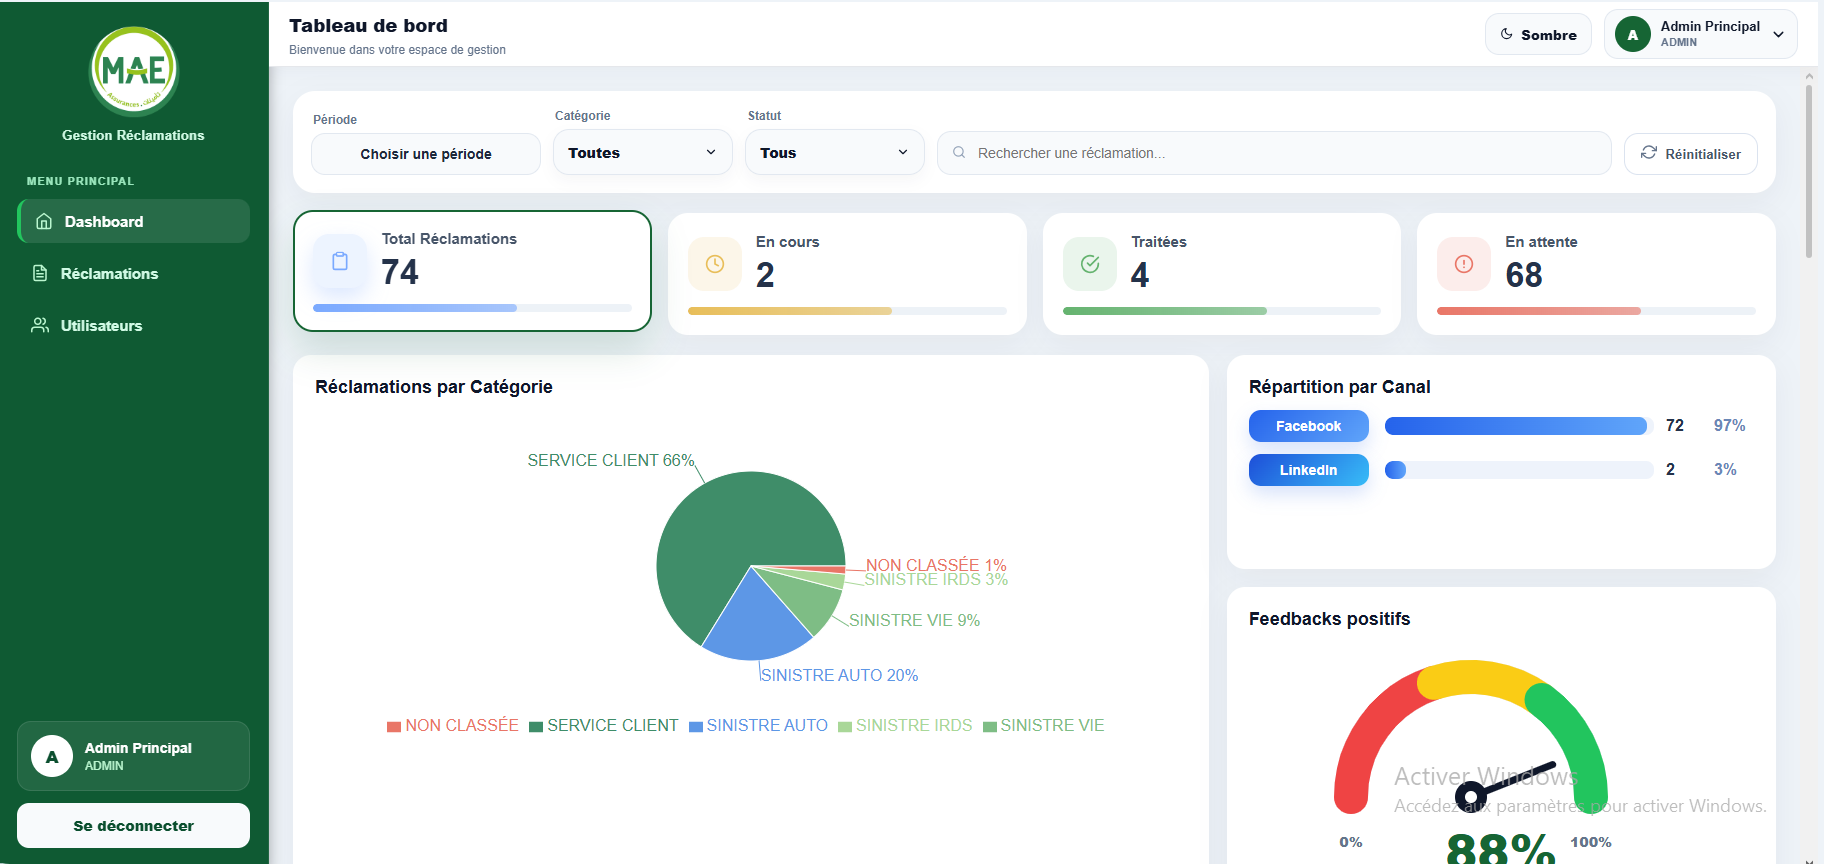
\includegraphics[width=1\linewidth]{interface.png}
    \caption{Interface principale de la plateforme}
    \label{fig:interface_principale}
\end{figure}

\section{Pages principales}

Cette section présente les principales interfaces développées dans la plateforme. Chaque page assure une fonctionnalité spécifique du système et facilite l’interaction entre les utilisateurs et l’application.

\subsection{Page de connexion}

La page de connexion permet aux utilisateurs d’accéder à la plateforme de manière sécurisée. L’utilisateur doit saisir son adresse email ainsi que son mot de passe afin d’être authentifié par le système.

Cette interface constitue le point d’entrée de l’application et garantit un accès sécurisé aux différentes fonctionnalités selon le rôle de l’utilisateur.

\begin{figure}[H]
    \centering
    
\includegraphics[width=0.75\textwidth]{login.png}
    \caption{Page de connexion}
    \label{fig:login_page}
\end{figure}

\subsection{Tableau de bord principal}

Après authentification, l’utilisateur accède au dashboard principal de la plateforme. Cette interface représente la page centrale du système et offre une vue globale sur les réclamations ainsi que sur les principaux indicateurs de performance.

Le dashboard affiche plusieurs statistiques importantes, notamment le nombre total de réclamations, les réclamations en attente, en cours de traitement et traitées. Il intègre également des graphiques et des outils de visualisation permettant d’analyser les données selon différentes catégories et canaux de communication.

Le dashboard permet aussi un accès rapide aux réclamations récentes ainsi qu’aux différentes fonctionnalités de la plateforme, facilitant ainsi le suivi et la gestion des réclamations.


\subsection{Visualisation et analyse des données}

La plateforme intègre plusieurs outils de visualisation permettant d’analyser les données liées aux réclamations et aux agences de la MAE.

Des graphiques statistiques sont utilisés afin de représenter l’évolution des réclamations, les temps de traitement ainsi que la répartition des réclamations selon différentes catégories et canaux. Une carte interactive permet également de visualiser les agences MAE réparties sur le territoire tunisien.

Ces éléments facilitent l’analyse des données et aident les utilisateurs à suivre les performances du système de manière claire et intuitive.

\begin{figure}[H]
    \centering
    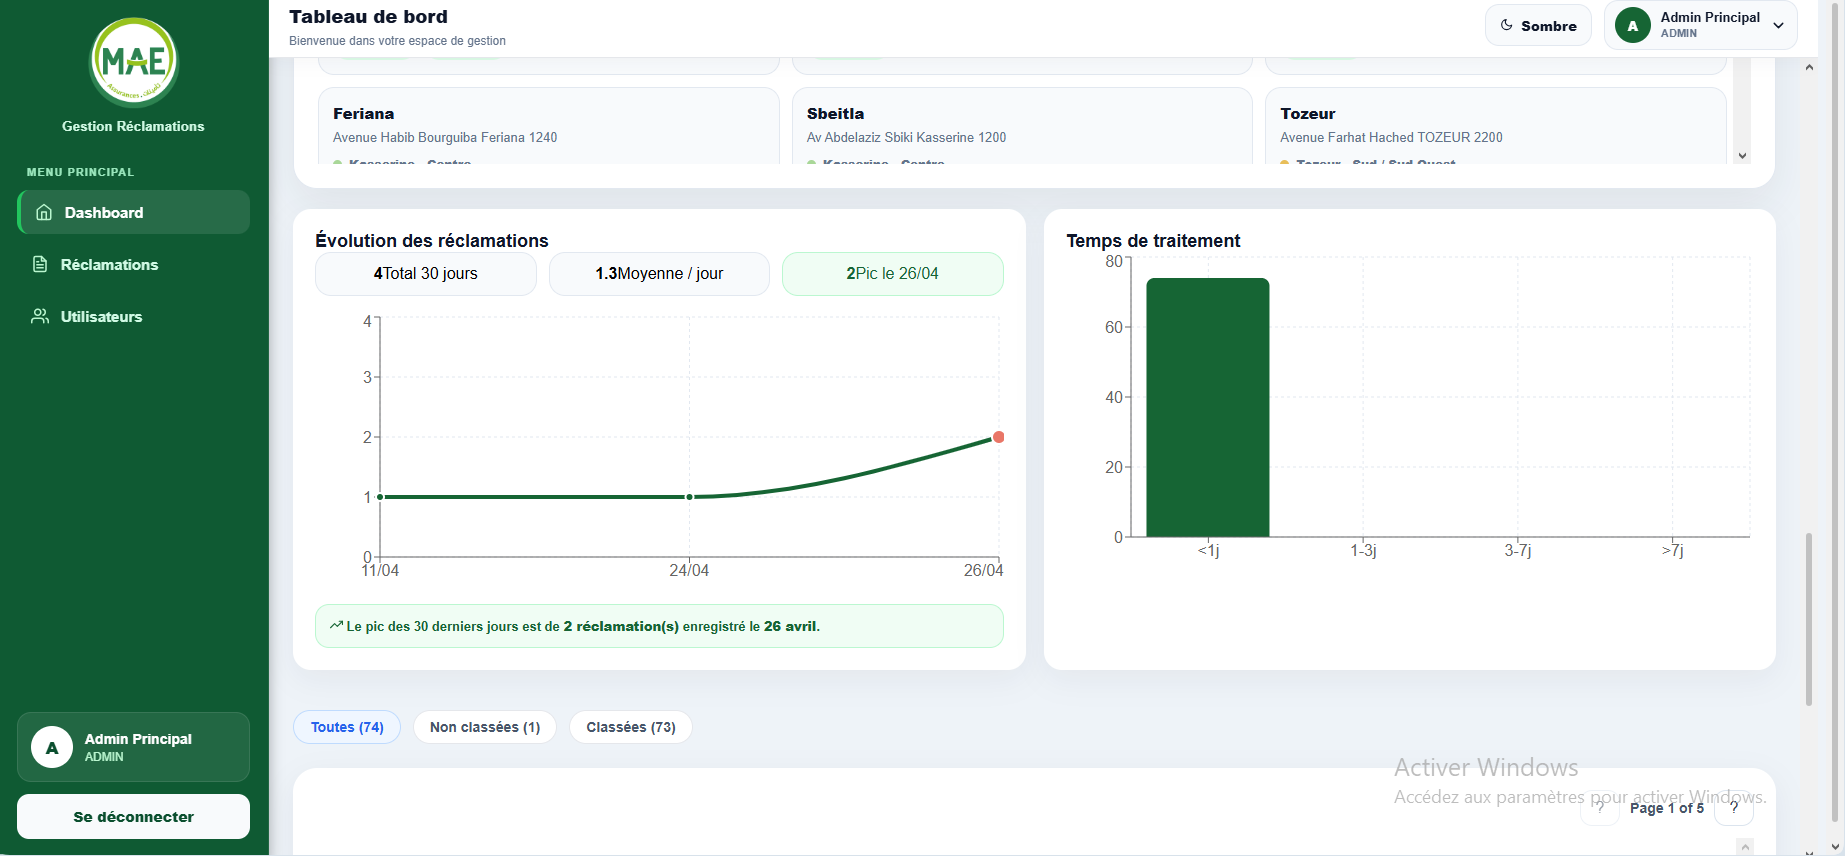
\includegraphics[width=\textwidth]{analyse_dashboard.png}
  \caption{Graphiques de visualisation et d’analyse des réclamations}
    \label{fig:analyse_dashboard}
\end{figure}

\subsection{Réseau et annuaire des agences}

La plateforme propose également un espace dédié à la visualisation du réseau des agences MAE en Tunisie.

Une carte interactive permet de localiser les agences tandis qu’un annuaire facilite la recherche des coordonnées des différentes agences selon plusieurs critères. Cette fonctionnalité améliore l’accès aux informations et facilite la consultation des données relatives aux agences.

\begin{figure}[H]
    \centering
    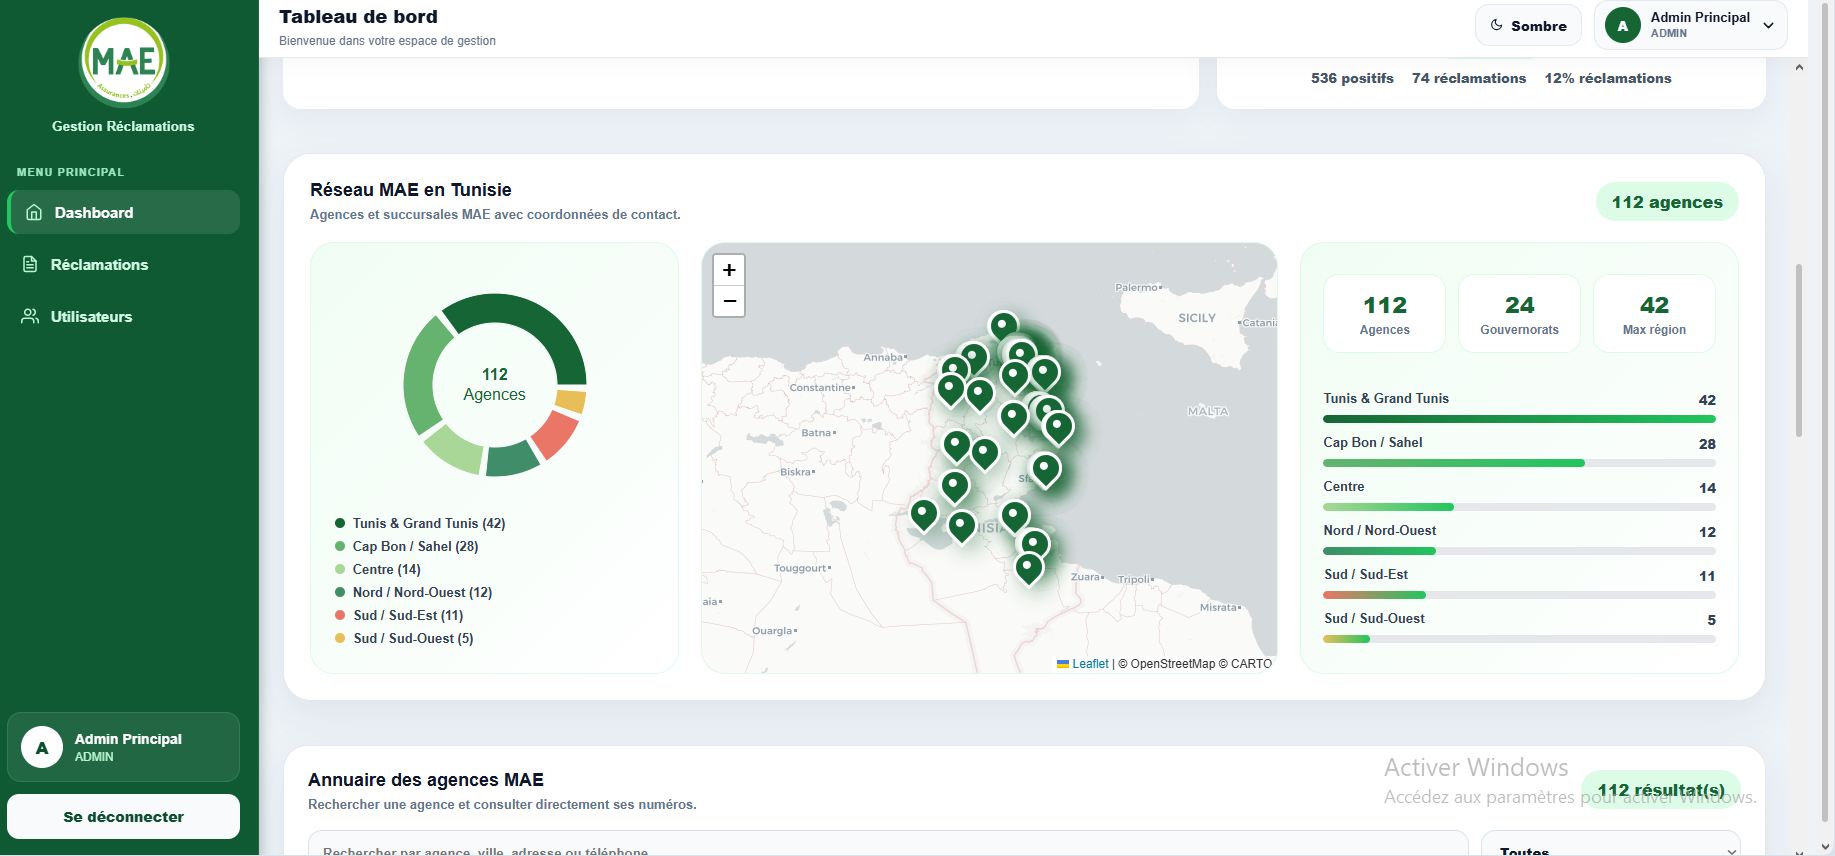
\includegraphics[width=\textwidth]{reseau_agences.png}
    \caption{Réseau des agences MAE}
    \label{fig:reseau_agences}
\end{figure}

\begin{figure}[H]
    \centering
    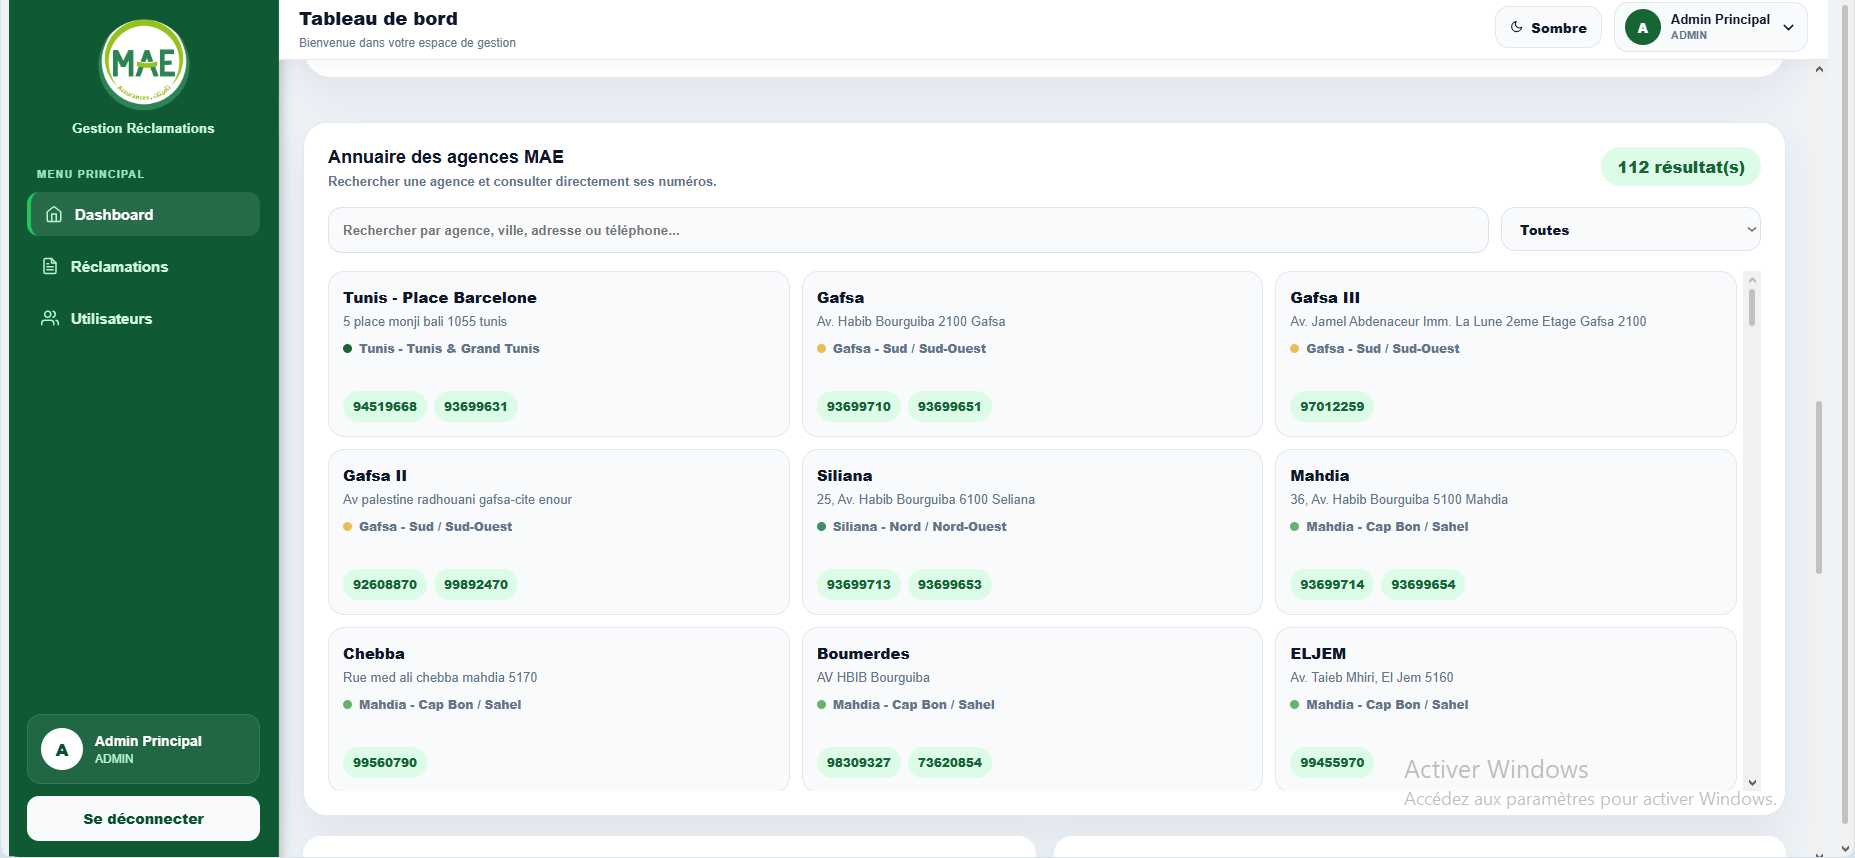
\includegraphics[width=\textwidth]{annuaire_agences.png}
    \caption{Annuaire des agences}
    \label{fig:annuaire_agences}
\end{figure}

\subsection{Gestion des réclamations}

La plateforme permet de consulter et gérer les réclamations à travers une interface dédiée. Cette page affiche les différentes réclamations sous forme de tableau contenant plusieurs informations importantes, telles que l’identifiant, le contenu de la réclamation, la catégorie, le canal, la date, le statut et le niveau d’urgence.

Les utilisateurs peuvent rechercher, filtrer et consulter les réclamations afin de faciliter leur traitement et leur suivi.

\begin{figure}[H]
    \centering
    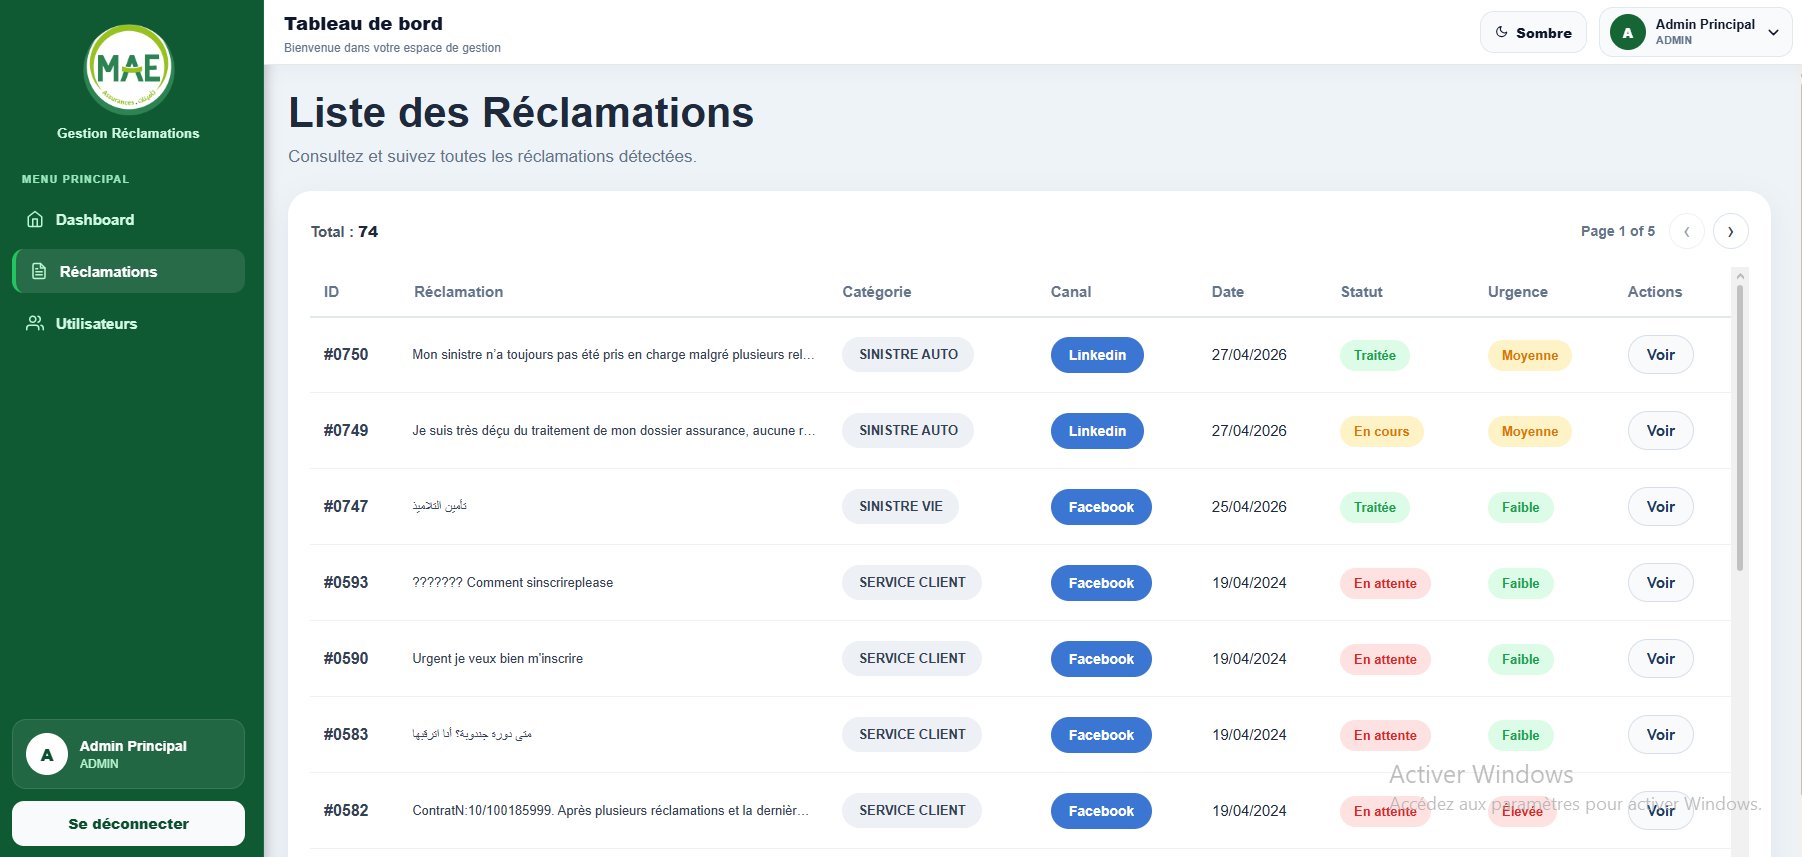
\includegraphics[width=\textwidth]{table_reclamations2.png}
    \caption{Gestion des réclamations}
    \label{fig:gestion_reclamations}
\end{figure}
\subsection{Détail d’une réclamation}

La plateforme permet également d’accéder à une vue détaillée d’une réclamation afin de consulter l’ensemble des informations associées.

Cette interface affiche plusieurs éléments importants tels que la source de la réclamation, la catégorie, le statut, le niveau d’urgence, les dates de traitement ainsi que l’historique complet des actions effectuées.

L’utilisateur peut également consulter le contenu complet de la réclamation et ajouter des notes internes afin de faciliter le suivi et le traitement des demandes.
\begin{figure}[H]
    \centering
    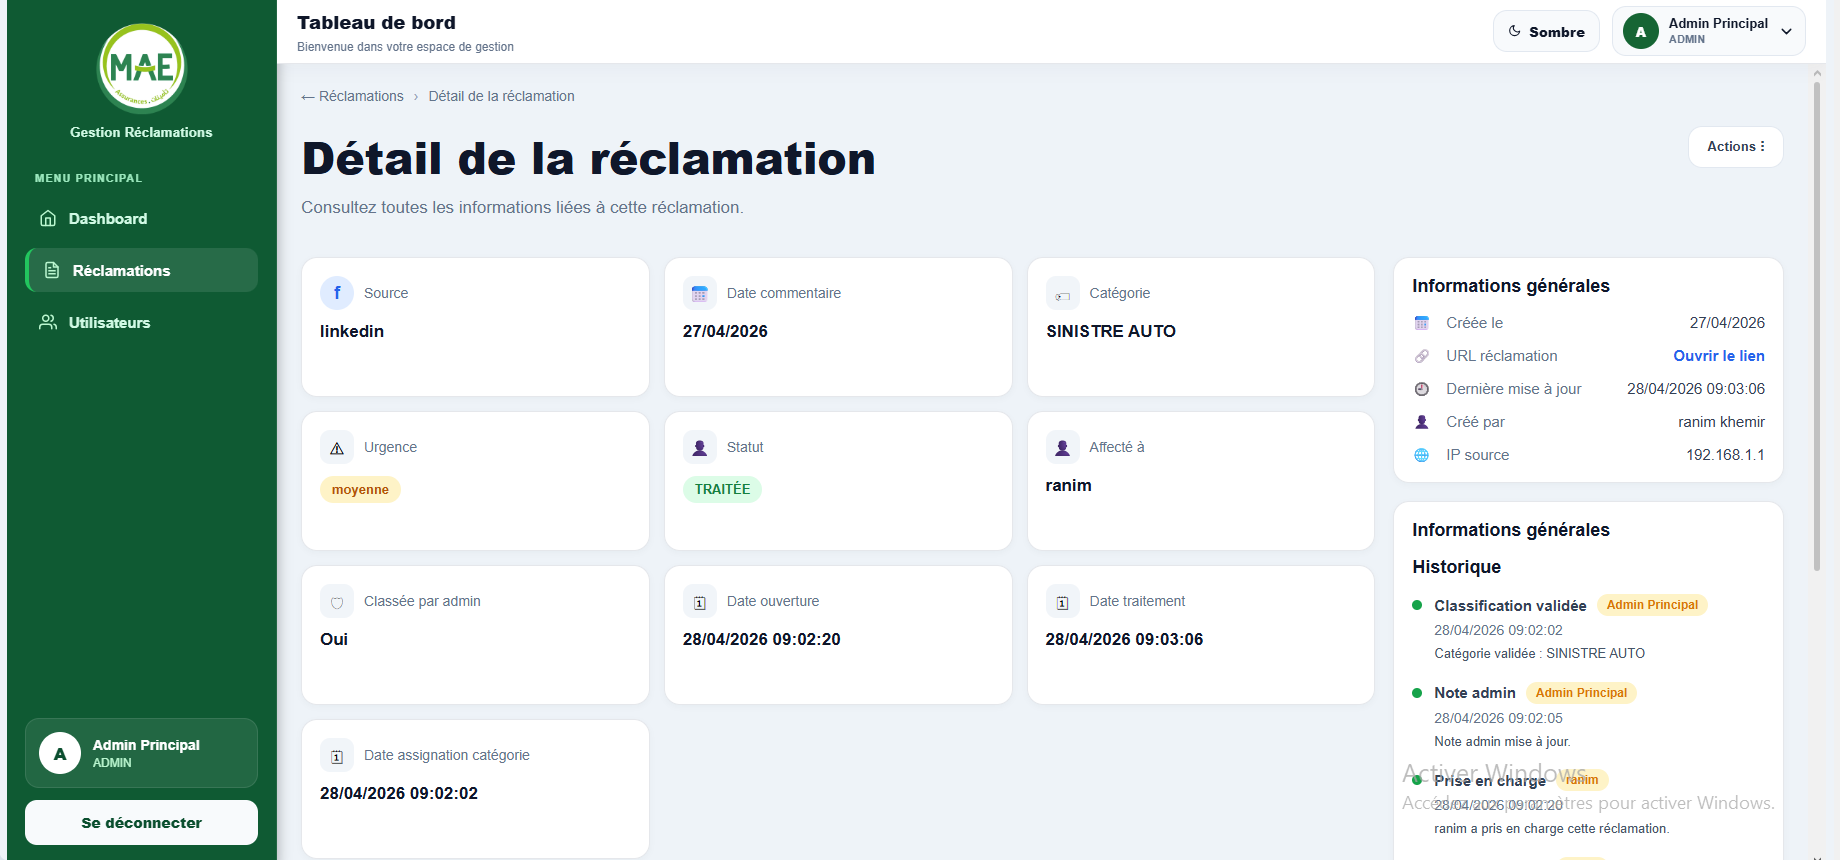
\includegraphics[width=\textwidth]{detail_reclamation_1.png}
    \caption{Informations générales d’une réclamation}
    \label{fig:detail_reclamation_1}
\end{figure}

\begin{figure}[H]
    \centering
    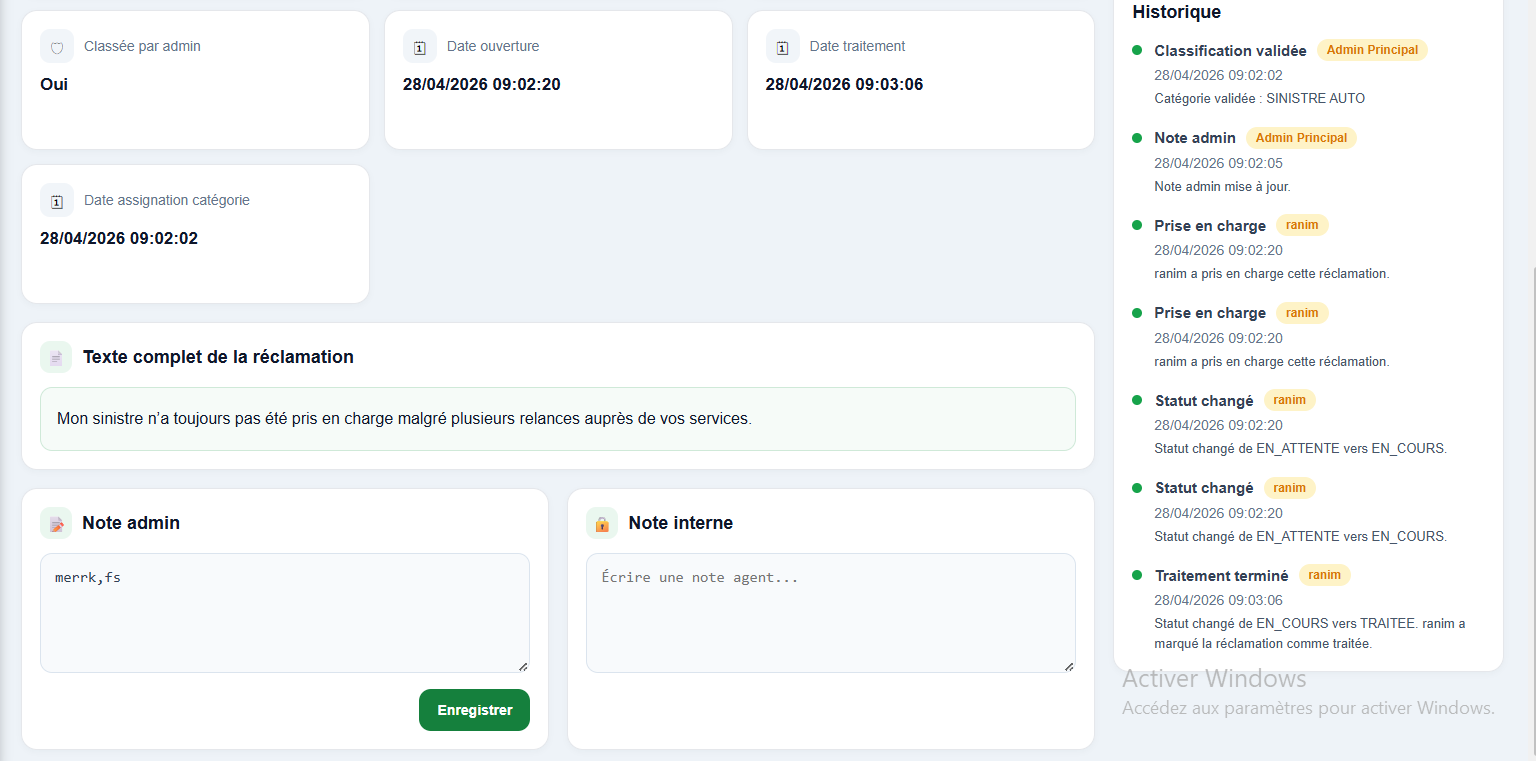
\includegraphics[width=\textwidth]{detail_reclamation_2.png}
    \caption{Suivi et traitement d’une réclamation}
    \label{fig:detail_reclamation_2}
\end{figure}

\section{Fonctionnalités implémentées}
\subsection{Différences entre l’interface agent et l’interface administrateur}

L’interface de la plateforme est adaptée selon le rôle de l’utilisateur connecté. Après authentification, le système identifie le rôle de l’utilisateur afin d’afficher les fonctionnalités autorisées.

L’agent dispose principalement des fonctionnalités liées au suivi opérationnel des réclamations. Il peut consulter la liste des réclamations, rechercher et filtrer les données, accéder au détail d’une réclamation, ajouter des notes internes et modifier le statut de traitement.

L’administrateur dispose de droits plus étendus. En plus de la consultation des réclamations et des indicateurs, il peut gérer les comptes utilisateurs, ajouter ou modifier des agents, activer ou désactiver des comptes et classifier manuellement les réclamations lorsque le système ne parvient pas à attribuer une catégorie avec une confiance suffisante.

Cette distinction permet de limiter l’accès aux fonctionnalités sensibles et d’adapter l’expérience utilisateur aux responsabilités de chaque rôle.

\subsection{Authentification et contrôle d’accès}

La plateforme intègre un système d’authentification sécurisé permettant de contrôler l’accès aux différentes fonctionnalités de l’application.

Chaque utilisateur doit se connecter à l’aide de son adresse email et de son mot de passe afin d’accéder à la plateforme. Après authentification, le système attribue les droits d’accès selon le rôle de l’utilisateur, notamment administrateur ou agent.

Ce mécanisme permet de protéger les données et d’assurer une gestion sécurisée des accès.

\begin{figure}[H]
    \centering
    
\includegraphics[width=0.55\textwidth]{login_page1.png}
    \caption{Interface de connexion}
    \label{fig:login_auth}
\end{figure}
\clearpage
La plateforme propose également une fonctionnalité de réinitialisation du mot de passe permettant aux utilisateurs de récupérer l’accès à leur compte en cas d’oubli du mot de passe.

\begin{figure}[H]
    \centering
    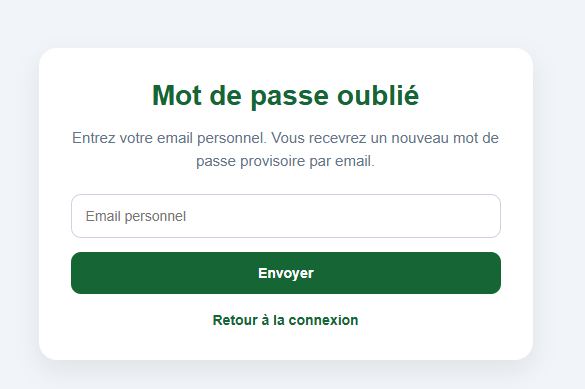
\includegraphics[width=0.55\textwidth]{forgot_password.png}
    \caption{Réinitialisation du mot de passe}
    \label{fig:forgot_password}
\end{figure}
\subsection{Visualisation des données}

Des outils de visualisation ont été intégrés afin de faciliter l’analyse des données liées aux réclamations et aux agences.

La plateforme propose plusieurs graphiques et indicateurs statistiques permettant de suivre l’évolution des réclamations, les performances du traitement ainsi que la répartition des données selon différentes catégories et canaux.

Ces visualisations permettent aux utilisateurs d’obtenir une vue globale sur l’activité du système et d’identifier rapidement les informations importantes grâce à une représentation graphique claire et intuitive.

\begin{figure}[H]
    \centering
    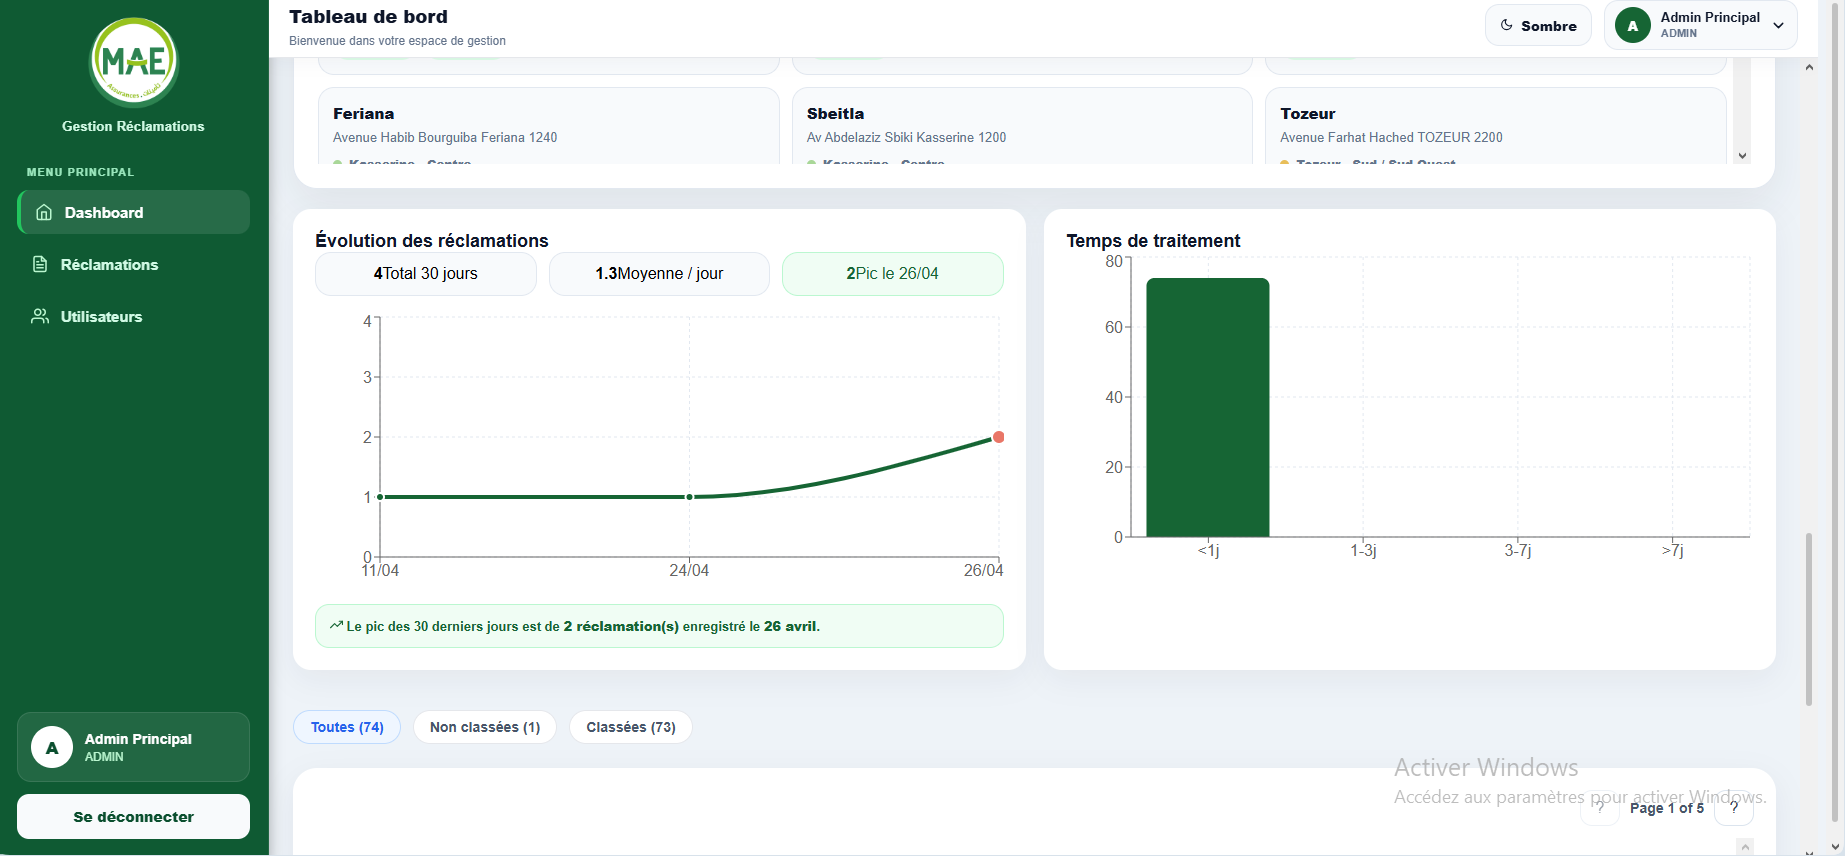
\includegraphics[width=\textwidth]{analyse_dashboard.png}
    \caption{Visualisation statistique des réclamations}
    \label{fig:data_visualisation}
\end{figure}
\subsection{Gestion des utilisateurs}

La plateforme permet à l’administrateur de gérer les différents comptes utilisateurs à travers une interface dédiée.

Cette fonctionnalité offre plusieurs opérations, notamment l’ajout, la modification et la suppression des agents. Le système permet également d’activer ou désactiver un compte utilisateur selon les besoins de gestion.

La page de gestion des utilisateurs affiche la liste des comptes existants ainsi que leurs informations principales, telles que le rôle, le statut et la catégorie assignée.

\begin{figure}[H]
    \centering
    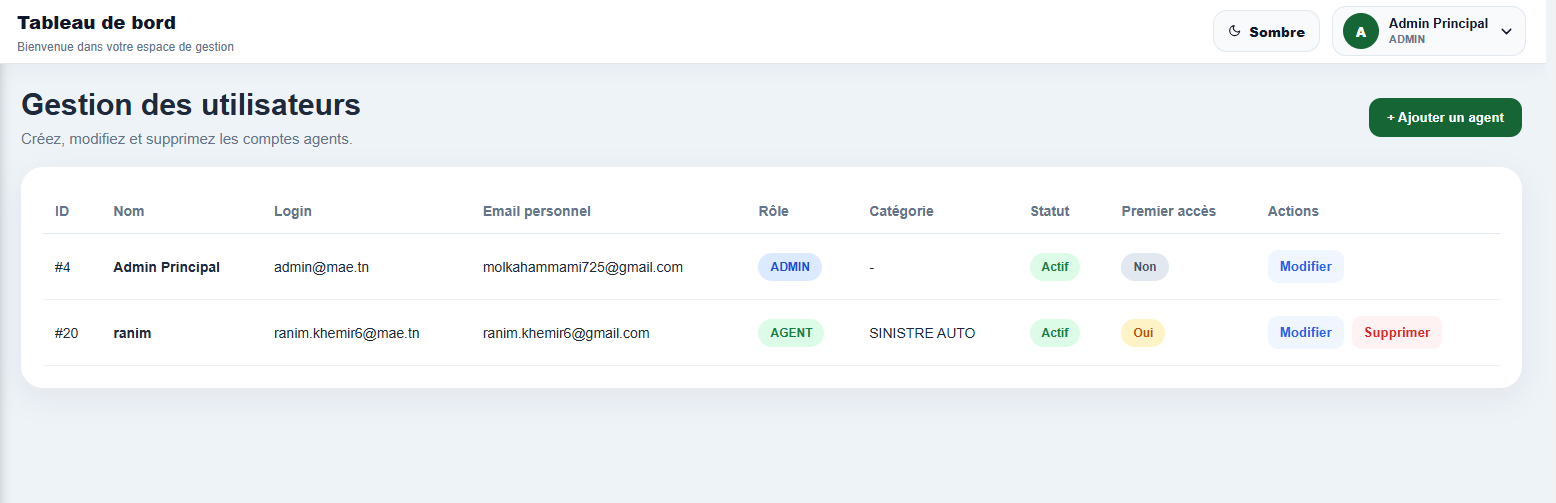
\includegraphics[width=\textwidth]{gestion_users.png}
    \caption{Gestion des utilisateurs}
    \label{fig:gestion_users}
\end{figure}

Lors de la création d’un nouvel utilisateur, l’administrateur doit renseigner plusieurs informations telles que le nom, l’adresse email, le rôle, la catégorie assignée ainsi qu’un mot de passe temporaire.

\begin{figure}[H]
    \centering
    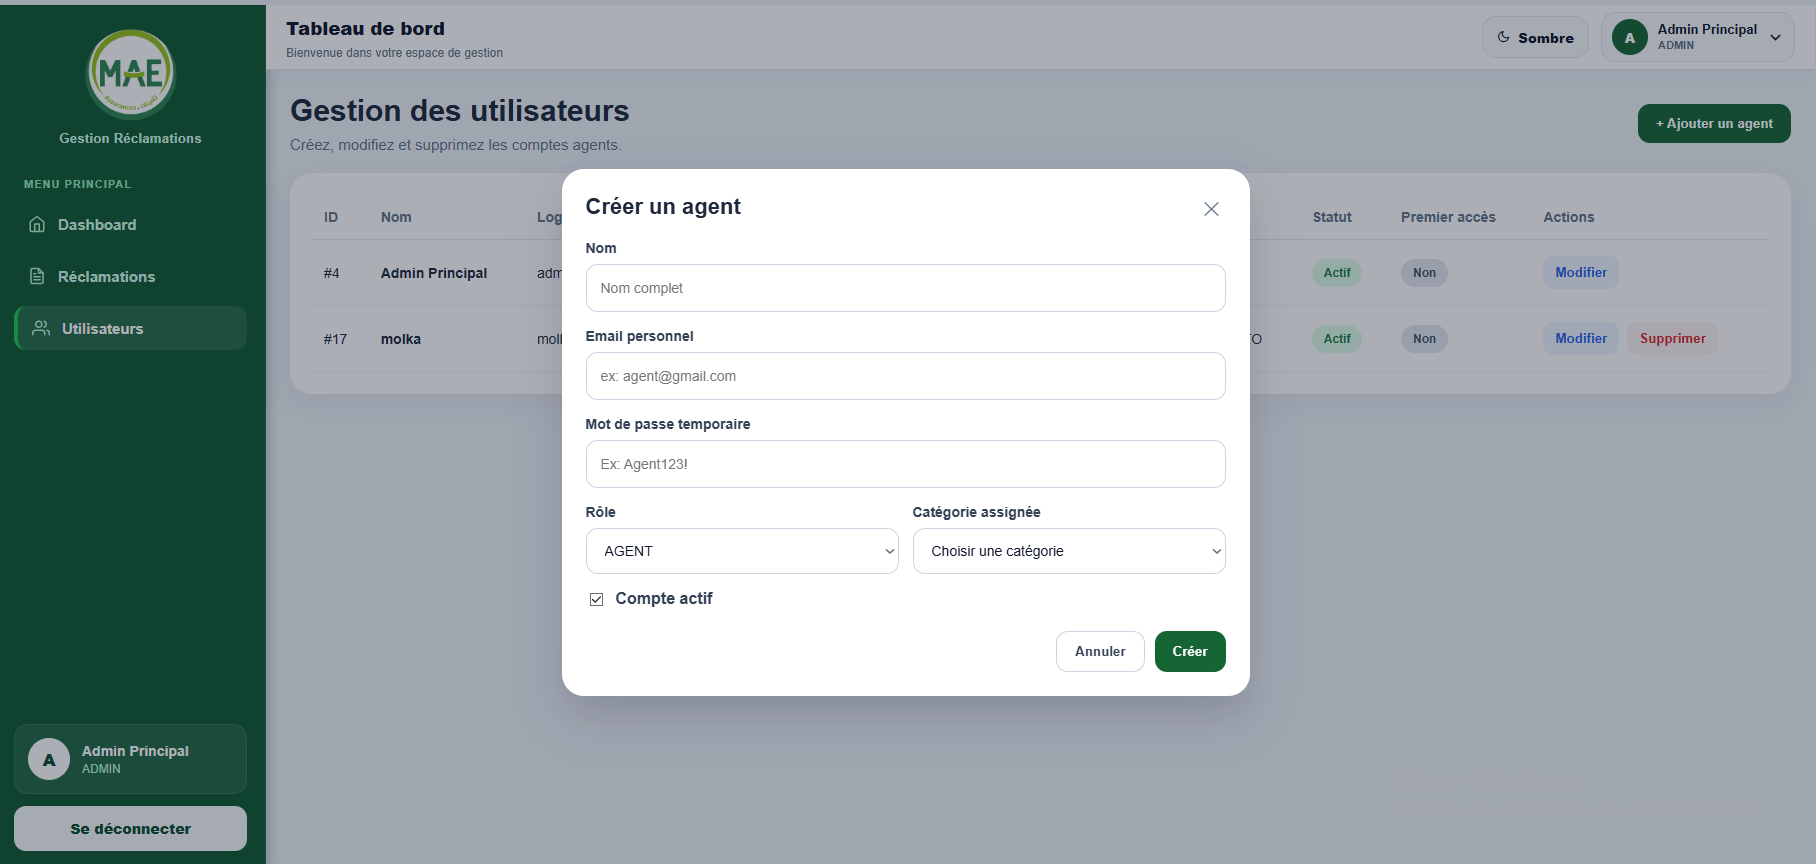
\includegraphics[width=0.85\textwidth]{ajout_utilisateur.png}
    \caption{Ajout d’un nouvel utilisateur}
    \label{fig:ajout_utilisateur}
\end{figure}
La plateforme permet également de modifier les informations d’un utilisateur existant. 
L’administrateur peut mettre à jour les informations personnelles, changer la catégorie assignée, réinitialiser le mot de passe temporaire ou modifier le statut du compte.

\begin{figure}[H]
    \centering
    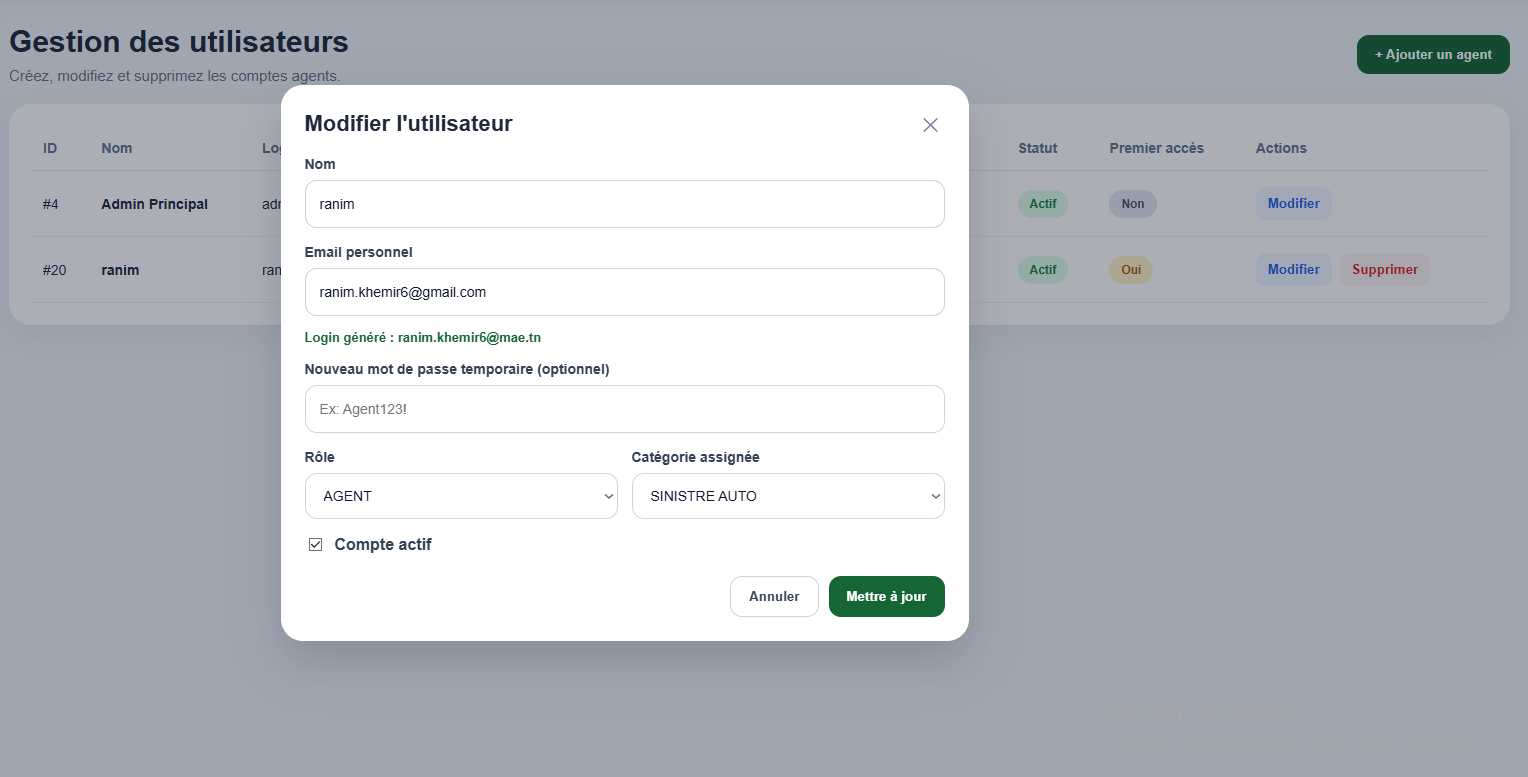
\includegraphics[width=0.85\textwidth]{modifier_utilisateur.png}
    \caption{Modification d’un utilisateur}
    \label{fig:modifier_utilisateur}
\end{figure}
\clearpage
\subsection{Notifications et envoi d’emails}

La plateforme intègre un système d’envoi automatique d’emails afin de faciliter la gestion des utilisateurs et renforcer la sécurité de l’application.

Lors de la création d’un nouveau compte agent par l’administrateur, un email est automatiquement envoyé contenant les informations de connexion ainsi qu’un mot de passe provisoire.

Le système permet également l’envoi d’un email de réinitialisation lorsqu’un utilisateur oublie son mot de passe. Un nouveau mot de passe temporaire est alors généré et transmis automatiquement à l’utilisateur concerné.

Ces mécanismes permettent d’améliorer la gestion des accès et d’assurer une meilleure sécurité des comptes utilisateurs.
\begin{figure}[H]
    \centering
    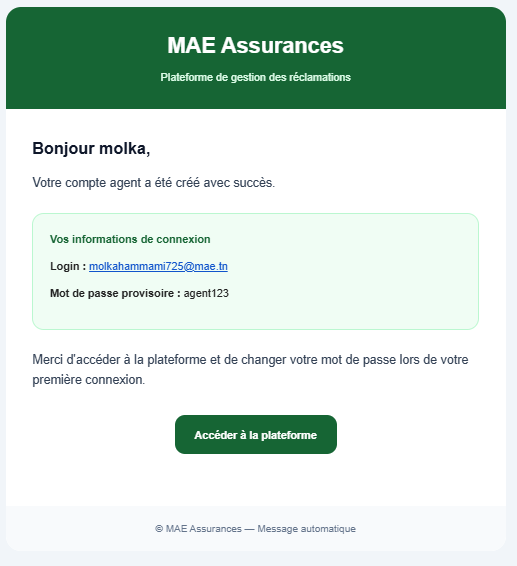
\includegraphics[width=0.8\textwidth]{mail_creation_agent.png}
    \caption{Email envoyé lors de la création d’un compte agent}
    \label{fig:mail_creation_agent}
\end{figure}
\begin{figure}[H]
    \centering
    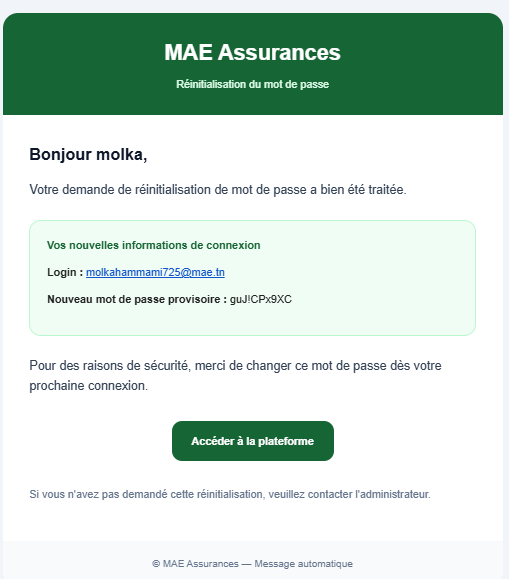
\includegraphics[width=0.8\textwidth]{mail_reset_password.png}
    \caption{Email de réinitialisation du mot de passe}
    \label{fig:mail_reset_password}
\end{figure}
\subsection{Sécurité des données}

La sécurité des données constitue un aspect important de la plateforme développée. Plusieurs mécanismes ont été intégrés afin de protéger les informations, contrôler l’accès aux fonctionnalités et assurer une utilisation sécurisée du système.

L’authentification repose sur l’utilisation de \textbf{JWT} (JSON Web Token). Après une connexion valide, le backend génère un token permettant d’identifier l’utilisateur lors de ses prochaines requêtes. Ce mécanisme évite de transmettre le mot de passe à chaque interaction avec l’API \cite{jwtio}.

Le contrôle d’accès est basé sur les rôles des utilisateurs, selon le principe \textbf{RBAC} (Role-Based Access Control). Ainsi, les fonctionnalités accessibles dépendent du rôle de l’utilisateur connecté. L’agent accède principalement aux fonctionnalités de consultation et de traitement des réclamations, tandis que l’administrateur dispose de droits supplémentaires pour gérer les utilisateurs et classifier manuellement certaines réclamations.

Les mots de passe ne sont pas stockés en clair dans la base de données. Ils sont protégés à l’aide d’un mécanisme de \textbf{hachage}, ce qui permet de renforcer la confidentialité des comptes utilisateurs.

Les routes sensibles de l’application sont destinées à être protégées par l’authentification et les permissions. Cela concerne notamment la gestion des utilisateurs, la modification des réclamations, l’ajout de notes internes et la classification manuelle.

La communication entre le frontend React et le backend Django est gérée à travers la configuration \textbf{CORS}, notamment durant la phase de développement où les deux parties peuvent fonctionner sur des ports différents \cite{mdncors}.

Enfin, la plateforme intègre un système d’envoi d’emails pour la création des comptes et la récupération du mot de passe. Lorsqu’un utilisateur oublie son mot de passe, un mot de passe provisoire est généré puis envoyé par email, ce qui facilite la récupération de l’accès au compte.

\section{Conclusion}

Dans ce chapitre, nous avons présenté le développement de la partie frontend de la plateforme de gestion des réclamations de la MAE Assurances.

Nous avons décrit les principales interfaces développées ainsi que les différentes fonctionnalités offertes aux utilisateurs, notamment la gestion des réclamations, la visualisation des données, le suivi des agences et la gestion des utilisateurs.

Les mécanismes d’authentification, de contrôle d’accès par rôle, de hachage des mots de passe, de protection des routes et de récupération par email contribuent également à renforcer la sécurité de la plateforme.

L’interface développée offre ainsi une expérience utilisateur fluide, intuitive et adaptée aux besoins des agents et des administrateurs.

% ===== CHAPITRE 7 =====
\chapter{Traitement intelligent des réclamations et analyse des résultats}

\section{Introduction}
Ce chapitre présente la partie intelligente du système, basée sur l’utilisation des techniques de traitement automatique du langage naturel (NLP).

L’objectif est d’analyser automatiquement les réclamations clients afin de les détecter, les classifier et d’estimer leur niveau d’urgence.

Nous décrivons dans ce chapitre les différentes étapes du traitement, depuis l’exploration des données jusqu’à l’analyse des résultats obtenus.

\section{Exploration et description des données}
L’exploration des données constitue une étape essentielle dans le processus de traitement des réclamations, car elle permet de mieux comprendre la nature, la structure et la qualité des données collectées.

Dans le cadre de ce projet, les données proviennent principalement des réseaux sociaux, notamment Facebook et LinkedIn, sous forme de commentaires clients. Ces données sont caractérisées par leur nature non structurée, leur diversité linguistique ainsi que la présence de bruit (erreurs, symboles, contenus inutiles).

\vspace{0.3cm}

\begin{itemize}
 \item\textbf{Nature des données}

Les données collectées sont principalement textuelles et contiennent :

\begin{itemize}
    \item le contenu du commentaire
    \item la date de publication
    \item la source (Facebook ou LinkedIn)
    \item l’auteur du commentaire
\end{itemize}

\end{itemize}
Ces informations sont extraites automatiquement à partir des plateformes sociales, comme illustré dans le processus d’extraction des commentaires.

\begin{itemize}
    \item \textbf{Problèmes identifiés}

L’analyse initiale des données a permis d’identifier plusieurs problèmes, notamment :

\begin{itemize}
    \item présence de commentaires vides ou non pertinents
    \item existence de contenu bruité (liens, emojis, ponctuation excessive)
    \item duplication de certains commentaires
    \item diversité linguistique (français, arabe, dialecte)
    \item variations dans la longueur des textes
\end{itemize}

\end{itemize}
Ces éléments peuvent impacter la qualité des résultats et nécessitent une étape de prétraitement.

\begin{itemize}
    \item \textbf{Nettoyage et préparation des données}


Afin d’améliorer la qualité des données, plusieurs opérations de nettoyage ont été appliquées :

\begin{itemize}
    \item suppression des URLs et des emails
    \item élimination des caractères spéciaux et de la ponctuation
    \item normalisation du texte (conversion en minuscules)
    \item suppression des espaces inutiles
\end{itemize}

\end{itemize}
Ces étapes sont réalisées automatiquement à l’aide d’un script de prétraitement dédié.

\begin{itemize}
    \item \textbf{Structuration des données}

Après nettoyage, les données sont transformées en un format structuré permettant leur exploitation dans les modèles de classification.

Chaque commentaire est enrichi par :

\begin{itemize}
    \item une version nettoyée du texte
    \item des informations associées (source, date, auteur)
\end{itemize}

\end{itemize}
Les données sont ensuite stockées dans une base de données PostgreSQL pour être utilisées dans les étapes suivantes du traitement.

\vspace{0.3cm}

Afin de mieux illustrer les différentes étapes du traitement des données, le pipeline global du système est présenté dans la figure suivante.

\begin{figure}[H]
    \centering
    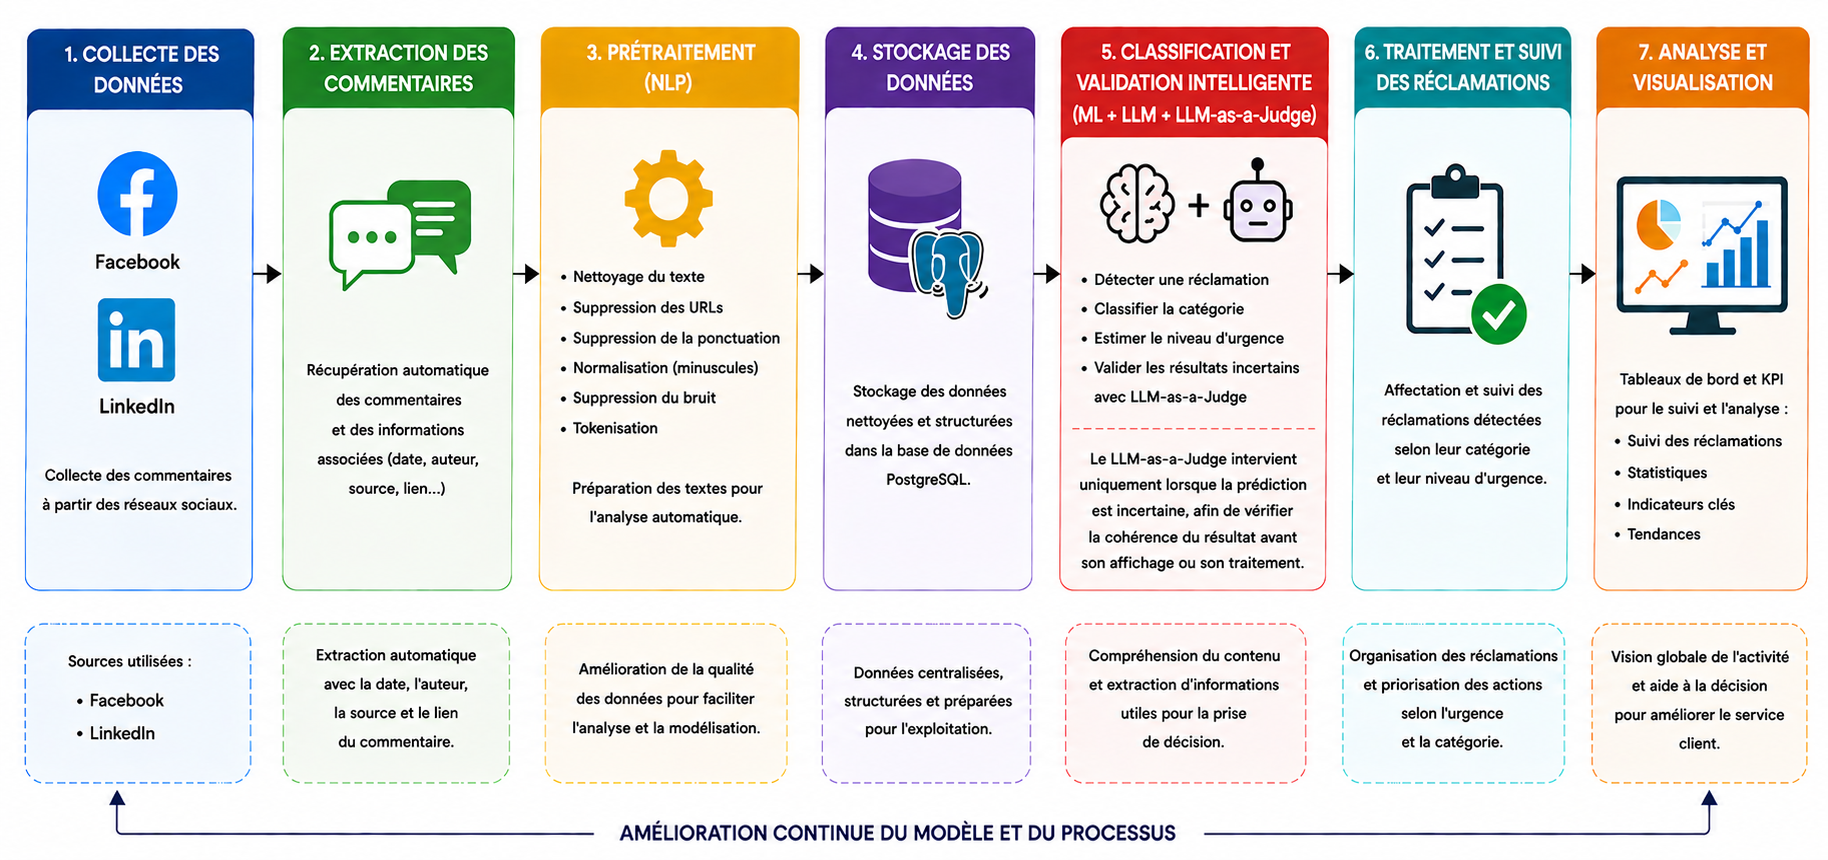
\includegraphics[width=1\linewidth]{pipeline de traitement.png}
    \caption{Pipeline de traitement des réclamations}
\end{figure}

Ce pipeline présente les différentes étapes du traitement des réclamations, depuis la collecte des commentaires à partir de Facebook et LinkedIn jusqu’à l’analyse et la visualisation des résultats. Les commentaires sont d’abord extraits avec leurs informations associées, puis nettoyés et préparés par le module NLP. Après leur stockage dans PostgreSQL, ils sont analysés par une approche hybride combinant Machine Learning, LLM et LLM-as-a-Judge. Cette étape permet de détecter les réclamations, de classifier leur catégorie, d’estimer leur niveau d’urgence et de valider les résultats incertains avant leur exploitation dans le suivi et le dashboard.

\section{Prétraitement NLP}
Le prétraitement des données constitue une étape fondamentale dans le processus de traitement automatique du langage naturel. Il vise à transformer les données textuelles brutes en un format exploitable par les modèles de classification.

Dans ce projet, les commentaires collectés à partir des réseaux sociaux sont souvent bruités, hétérogènes et non structurés. Il est donc nécessaire d’appliquer plusieurs opérations de nettoyage et de transformation afin d’améliorer la qualité des données et d’optimiser les performances des modèles.

\begin{itemize}
    \item \textbf{Nettoyage du texte}

La première étape consiste à nettoyer les données en supprimant les éléments inutiles ou perturbateurs. Les opérations suivantes ont été appliquées :

\begin{itemize}
    \item suppression des adresses email
    \item suppression des liens (URLs)
    \item suppression des hashtags
    \item élimination de la ponctuation
    \item suppression des caractères spéciaux
    \item suppression des espaces multiples
\end{itemize}
\end{itemize}
Ces opérations permettent de réduire le bruit et de conserver uniquement les informations pertinentes pour l’analyse.

\begin{itemize}
    \item \textbf{Normalisation}

La normalisation consiste à uniformiser le texte afin de faciliter son traitement. Dans ce cadre, les actions suivantes ont été réalisées :

\begin{itemize}
    \item conversion du texte en minuscules
    \item suppression des variations inutiles d’écriture
    \item simplification des structures textuelles
\end{itemize}
\end{itemize}
Cette étape permet d’éviter que des mots similaires soient interprétés différemment par le modèle.

\begin{itemize}
    \item \textbf{Nettoyage linguistique}
\end{itemize}

Les données collectées présentent une diversité linguistique importante, incluant le français, l’arabe standard et le dialecte. Cette diversité rend le traitement plus complexe et nécessite une simplification du texte afin d’en extraire les informations essentielles.

\begin{itemize}
    \item \textbf{Génération du texte nettoyé}
\end{itemize}

Après application des différentes étapes de prétraitement, une nouvelle version du texte est générée pour chaque commentaire, appelée \textbf{texte nettoyé (clean-text)}. Cette version est utilisée comme entrée principale des modèles de classification.

Ces opérations de prétraitement sont réalisées automatiquement à l’aide d’un script dédié , garantissant un traitement cohérent et reproductible des données.

\begin{itemize}
    \item \textbf{Importance du prétraitement}

Le prétraitement joue un rôle crucial dans la qualité des résultats obtenus. En effet, un texte bien nettoyé permet :

\begin{itemize}
    \item d’améliorer la précision des modèles
    \item de réduire les erreurs de classification
    \item d’optimiser les performances globales du système
\end{itemize}
\end{itemize}
\section{Modélisation et classification des données}
La modélisation constitue une étape clé dans le système de traitement intelligent des réclamations. Elle permet d’automatiser l’analyse des commentaires clients en utilisant des techniques de machine learning et des modèles de langage.

Dans ce projet, une approche hybride a été adoptée, combinant des modèles de machine learning classiques et un modèle de langage avancé (LLM), afin d’améliorer la précision et la robustesse des résultats.

\begin{itemize}
    \item \textbf{Mise en place des modèles}

Dans ce projet, trois modèles distincts ont été implémentés afin de traiter les différentes dimensions de la classification :

\begin{itemize}
    \item un modèle dédié à la détection des réclamations
    \item un modèle de classification des catégories
    \item un modèle d’estimation du niveau d’urgence
\end{itemize}
\end{itemize}

Ces modèles permettent de traiter les commentaires de manière progressive, en enrichissant chaque donnée avec des informations supplémentaires à chaque étape.

\begin{itemize}
    \item \textbf{Modèles de Machine Learning}

Une première approche basée sur le machine learning a été mise en place à l’aide de modèles supervisés.

\textbf{Vectorisation des données}

La méthode TF-IDF (Term Frequency - Inverse Document Frequency) \cite{tfidf} permet de représenter
l’importance d’un mot dans un document par rapport à l’ensemble du corpus.

Elle repose sur la combinaison de deux mesures :

\begin{equation}
TF\text{-}IDF(t,d) = TF(t,d) \times IDF(t)
\end{equation}

où :

- \(TF(t,d)\) représente la fréquence du terme \(t\) dans le document \(d\).

- \(IDF(t)\) mesure l’importance du terme dans le corpus global.

Cette technique permet d’attribuer un poids plus important aux termes significatifs du corpus tout en réduisant l’influence des mots fréquents peu informatifs.

\textbf{Modèles utilisés}

Les modèles suivants ont été entraînés :

\begin{enumerate}
    \item un modèle de classification des réclamations
    \item un modèle de classification des catégories
    \item un modèle de classification de l’urgence
\end{enumerate}

Ces modèles sont basés sur des algorithmes de type régression logistique, adaptés aux problèmes de classification textuelle \cite{logreg}.

Pour l’entraînement, le dataset a été divisé en deux parties : \textbf{80\%} des données ont été utilisées pour l’apprentissage et \textbf{20\%} pour le test. Cette séparation permet d’évaluer les modèles sur des données non vues pendant l’entraînement.

La vectorisation des textes a été réalisée avec la méthode \textbf{TF-IDF} en utilisant des n-grammes de taille \textbf{(1,2)}, ce qui permet de prendre en compte les mots isolés ainsi que certaines combinaisons de deux mots. Le modèle de détection des réclamations utilise \texttt{max\_features=5000}, le modèle de classification des catégories utilise \texttt{max\_features=7000}, et le modèle d’estimation de l’urgence utilise \texttt{max\_features=5000} \cite{tfidf}.

Afin de limiter l’impact du déséquilibre entre certaines classes, les modèles de régression logistique ont été entraînés avec le paramètre \texttt{class\_weight='balanced'}.


\textbf{Algorithme de classification}

Parmi les modèles utilisés, la régression logistique constitue une approche efficace pour la classification des données textuelles \cite{logreg}.

Ce modèle permet d’estimer la probabilité qu’une réclamation appartienne à une catégorie donnée.

\begin{equation}
P(y=1 \mid x) = \frac{1}{1 + e^{-z}}
\end{equation}

où $z$ représente une combinaison linéaire des variables d’entrée issues de la vectorisation TF-IDF.
\end{itemize}

Cette approche permet de transformer les données textuelles vectorisées en probabilités, facilitant ainsi la prise de décision finale.

\begin{itemize}
    \item \textbf{Limites du Machine Learning}

Bien que les modèles ML offrent de bonnes performances, ils présentent certaines limites :

\begin{itemize}
    \item difficulté à comprendre le contexte complexe
    \item sensibilité aux variations linguistiques
    \item limitation face aux textes ambigus ou courts
\end{itemize}
\end{itemize}

Ces limites ont motivé l’intégration d’une approche complémentaire basée sur un modèle de langage.

\begin{itemize}
    \item \textbf{Intégration d’un modèle LLM}

Un modèle de langage (LLM) a été intégré afin d’améliorer la compréhension des textes et la qualité des classifications \cite{ibmllm,hftransformers}.

Ce modèle permet :

\begin{itemize}
    \item d’analyser le contexte global du commentaire
    \item de mieux gérer les variations linguistiques
    \item de traiter les cas ambigus
\end{itemize}
\end{itemize}

Le modèle LLM est intégré via une API dédiée, qui retourne directement les résultats de classification sous forme structurée

\begin{itemize}
    \item \textbf{Approche hybride (Machine Learning + LLM)}

Afin d’améliorer les performances du système, une approche hybride a été adoptée. Cette approche combine les avantages du machine learning et des modèles de langage.

Le système repose sur un mécanisme de décision permettant de choisir dynamiquement la méthode la plus adaptée :

\begin{itemize}
    \item si le modèle ML est suffisamment confiant, sa prédiction est utilisée directement ;
    \item si le score de confiance lié à la détection de réclamation se situe dans la zone d’incertitude entre \textbf{0.40} et \textbf{0.60}, le système fait appel au LLM ;
    \item si le commentaire est détecté comme une réclamation mais que la confiance associée à la catégorie est inférieure à \textbf{0.55}, le système fait également appel au LLM ;
    \item le LLM propose alors une prédiction structurée contenant le type du commentaire, la catégorie et le niveau d’urgence.
\end{itemize}

\end{itemize}

Cette stratégie permet de tirer parti de la rapidité du machine learning et de la capacité de compréhension contextuelle du modèle de langage.

\begin{itemize}
    \item \textbf{Règles métier}
\end{itemize}

En complément des modèles de classification, des règles métier ont été intégrées afin d’améliorer la cohérence et la précision des résultats.

Ces règles permettent d’orienter le processus de classification en tenant compte de certains éléments contextuels et linguistiques présents dans les commentaires. Elles interviennent principalement pour affiner les décisions des modèles, notamment dans les cas ambigus ou lorsque les prédictions sont incertaines.

L’intégration de ces règles contribue à renforcer la fiabilité du système en assurant une meilleure adéquation entre les résultats obtenus et les besoins métier. Elles permettent également d’introduire une logique experte dans le processus de traitement automatique.

\begin{itemize}
    \item \textbf{Résultat du traitement}

À l’issue du processus de classification, chaque commentaire est enrichi avec plusieurs informations structurées, notamment :

\begin{itemize}
    \item le type : réclamation ou non
    \item la catégorie associée
    \item le niveau d’urgence
\end{itemize}
\end{itemize}

Ces informations sont ensuite exploitées dans le système pour faciliter la gestion et le suivi des réclamations.

Afin de mieux présenter la démarche adoptée pour la construction du modèle de classification, le processus global est illustré dans la figure suivante.

\begin{figure}[H]
    \centering
    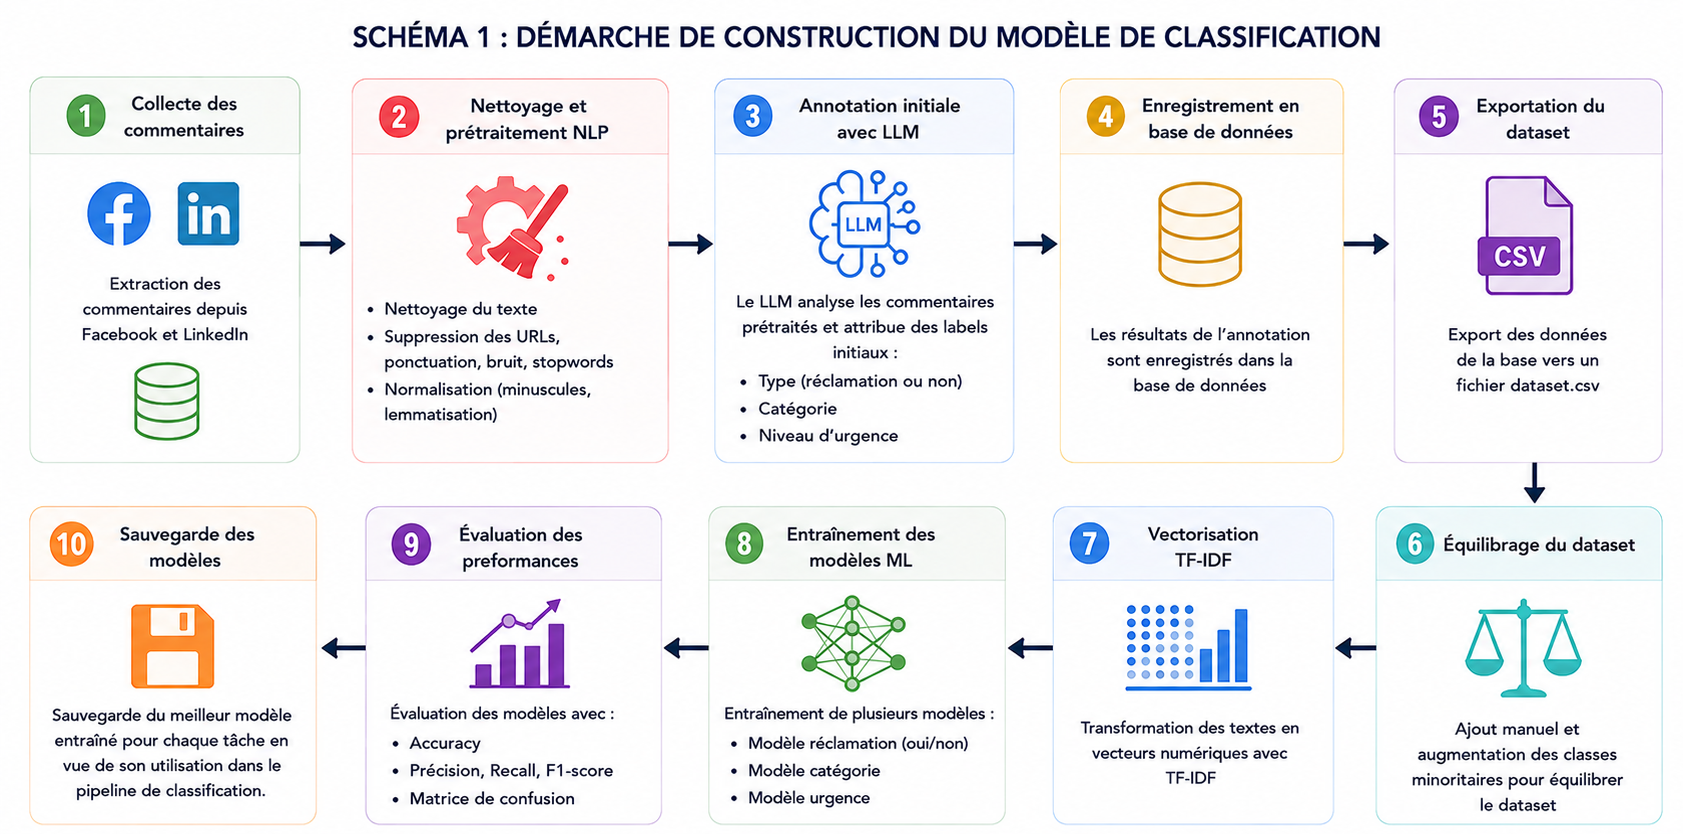
\includegraphics[width=1\linewidth]{demarche du construction du modele.png}
    \caption{Démarche de construction du modèle de classification}
\end{figure}

La figure ci-dessus illustre la démarche suivie pour construire les modèles de classification. Le processus commence par la collecte des commentaires depuis Facebook et LinkedIn, suivie d’une phase de nettoyage et de prétraitement NLP afin d’obtenir des textes exploitables. Les commentaires prétraités sont ensuite annotés initialement à l’aide d’un LLM, qui attribue les labels nécessaires : type de commentaire, catégorie et niveau d’urgence.

Les résultats de cette annotation sont enregistrés dans la base de données, puis exportés sous forme de dataset afin d’être utilisés pour l’apprentissage supervisé. Une étape d’équilibrage est ensuite réalisée pour réduire l’impact des classes minoritaires. Les textes sont transformés en vecteurs numériques à l’aide de la méthode TF-IDF, puis plusieurs modèles ML sont entraînés : un modèle de détection des réclamations, un modèle de classification des catégories et un modèle d’estimation de l’urgence.

Enfin, les performances des modèles sont évaluées à l’aide de métriques telles que l’accuracy, la précision, le recall, le F1-score et la matrice de confusion. Les meilleurs modèles et leurs vectorizers sont sauvegardés afin d’être intégrés dans le pipeline de classification.

\section{Résultats d’entraînement des modèles}

Pour évaluer les performances des modèles, plusieurs métriques ont été utilisées :

\textbf{L’accuracy} représente le taux global de prédictions correctes parmi l’ensemble des exemples testés. Elle donne une vision générale de la performance du modèle \cite{metrics}.

\begin{equation}
Accuracy = \frac{TP + TN}{TP + TN + FP + FN}
\end{equation}

\textbf{La précision} mesure la proportion de prédictions correctes parmi les éléments que le modèle a classés dans une catégorie donnée. Une précision élevée signifie que le modèle fait peu de fausses prédictions pour cette classe \cite{metrics}.

\begin{equation}
\text{Précision} = \frac{TP}{TP + FP}
\end{equation}


\textbf{Le recall}, ou \textbf{rappel}, mesure la capacité du modèle à retrouver tous les exemples appartenant réellement à une classe. Un recall élevé signifie que le modèle détecte correctement la majorité des exemples de cette classe \cite{metrics}.

\begin{equation}
Recall = \frac{TP}{TP + FN}
\end{equation}

\textbf{Le F1-score} est la moyenne harmonique entre la précision et le recall. Il permet d’obtenir une mesure équilibrée, particulièrement utile lorsque les classes ne sont pas parfaitement équilibrées \cite{metrics}.

\begin{equation}
F1\text{-}score =
2 \times \frac{\text{Précision} \times \text{Recall}}
{\text{Précision} + \text{Recall}}
\end{equation}

Avec :

\textbf{TP :} vrais positifs

\textbf{TN :} vrais négatifs

\textbf{FP :} faux positifs

\textbf{FN :} faux négatifs


\begin{table}[H]
\centering
\caption{Résultats du modèle de détection des réclamations}
\begin{tabular}{|l|c|c|c|}
\hline
Classe & Précision & Recall & F1-score \\
\hline
non\_reclamation & 0.81 & 0.85 & 0.83 \\
reclamation & 0.89 & 0.86 & 0.88 \\
\hline
Accuracy & -- & -- & 0.86 \\
\hline
\end{tabular}
\end{table}


\begin{table}[H]
\centering
\caption{Résultats du modèle de classification des catégories}
\begin{tabular}{|l|c|c|c|}
\hline
Classe & Précision & Recall & F1-score \\
\hline
SERVICE CLIENT & 0.74 & 1.00 & 0.85 \\
SINISTRE AUTO & 0.89 & 0.80 & 0.84 \\
SINISTRE IRDS & 0.90 & 0.69 & 0.78 \\
SINISTRE VIE & 0.86 & 0.67 & 0.75 \\
\hline
Accuracy & - & - & 0.82 \\
\hline
\end{tabular}
\end{table}


\begin{table}[H]
\centering
\caption{Résultats du modèle d'estimation de l'urgence}
\begin{tabular}{|l|c|c|c|}
\hline
Classe & Précision & Recall & F1-score \\
\hline
élevée & 0.90 & 0.72 & 0.80 \\
faible & 0.79 & 0.85 & 0.81 \\
moyenne & 0.53 & 0.73 & 0.62 \\
\hline
Accuracy & -- & -- & 0.76 \\
\hline
\end{tabular}
\end{table}


Les résultats montrent que le modèle de détection des réclamations obtient de bonnes performances, avec une \textbf{accuracy} de \textbf{0.86} et un \textbf{F1-score} pondéré de \textbf{0.86}. Il distingue correctement les réclamations des commentaires non réclamants.

Pour la classification des catégories, le modèle obtient une \textbf{accuracy} de \textbf{0.82}. La catégorie SERVICE CLIENT présente un \textbf{rappel} de \textbf{1.00}, ce qui signifie que tous les exemples de cette classe dans l’ensemble de test ont été correctement détectés. Les catégories SINISTRE AUTO, SINISTRE IRDS et SINISTRE VIE obtiennent également des résultats acceptables, avec des \textbf{F1-scores} respectifs de \textbf{0.84}, \textbf{0.78} et \textbf{0.75}.

Pour l’estimation de l’urgence, le modèle obtient une \textbf{accuracy} de\textbf{ 0.76}. Les classes élevée et faible sont relativement bien reconnues, avec des \textbf{F1-scores} de \textbf{0.80} et \textbf{0.81}. La classe moyenne est plus difficile à classifier, avec un \textbf{F1-score} de \textbf{0.62}, car elle représente souvent des situations intermédiaires moins clairement exprimées dans les commentaires.


L’analyse par classe montre que le modèle de détection des réclamations obtient des résultats équilibrés entre les deux classes. La classe \texttt{reclamation} présente un F1-score de \textbf{0.88}, ce qui montre que le modèle identifie correctement la majorité des commentaires nécessitant un traitement.

Pour la classification des catégories, la classe \texttt{SERVICE CLIENT} obtient le meilleur rappel avec une valeur de \textbf{1.00}. Cela signifie que les exemples de cette classe sont bien retrouvés par le modèle. En revanche, les classes \texttt{SINISTRE IRDS} et \texttt{SINISTRE VIE} présentent des rappels plus faibles, respectivement \textbf{0.69} et \textbf{0.67}, ce qui peut s’expliquer par la proximité sémantique de certains commentaires et par le nombre limité d’exemples disponibles.

Concernant l’urgence, les classes \texttt{faible} et \texttt{elevee} sont mieux reconnues que la classe \texttt{moyenne}. Cette dernière obtient un F1-score de \textbf{0.62}, car elle correspond souvent à des situations intermédiaires, moins explicites que les cas clairement simples ou critiques.


\section{Score d’urgence}
L’estimation du score d’urgence constitue une étape importante dans le traitement des réclamations, car elle permet de prioriser leur prise en charge en fonction de leur importance.

Dans ce projet, chaque réclamation est associée à un niveau d’urgence, permettant d’identifier les cas nécessitant une intervention rapide.

\begin{itemize}
    \item \textbf{Objectif du score d’urgence}

L’objectif principal est de classer les réclamations selon leur degré de priorité afin de :

\begin{itemize}
    \item faciliter la prise de décision
    \item améliorer la réactivité du système
    \item optimiser la gestion des réclamations
\end{itemize}
\end{itemize}

\begin{itemize}
    \item \textbf{Niveaux d’urgence}

Le système distingue généralement trois niveaux d’urgence :

\begin{enumerate}
    \item \textbf{faible :} pour les demandes simples ou les requêtes d’information
    \item \textbf{moyenne :} pour les problèmes nécessitant une intervention mais sans caractère critique
    \item \textbf{élevée :} pour les situations urgentes nécessitant une prise en charge rapide
\end{enumerate}
\end{itemize}

\begin{itemize}
    \item \textbf{Méthode d’estimation}
\end{itemize}

L’estimation du score d’urgence est réalisée automatiquement à l’aide d’un modèle de classification intégré dans le système.

Ce modèle analyse le contenu du commentaire afin de détecter des indices reflétant le degré d’urgence, tels que la nature du problème, le niveau de frustration exprimé ou l’impact de la situation.

Dans certains cas, notamment lorsque la prédiction du modèle est incertaine, le système peut faire appel au modèle de langage (LLM) afin d’améliorer l’évaluation.

\begin{itemize}
    \item \textbf{Intégration dans le système}

Le score d’urgence est calculé en même temps que les autres informations (type de réclamation et catégorie), et est directement associé à chaque commentaire.

Ces informations sont ensuite utilisées pour :

\begin{itemize}
    \item prioriser les réclamations dans le système
    \item faciliter leur traitement par les agents
    \item améliorer le suivi global des cas
\end{itemize}
\end{itemize}

\begin{itemize}
    \item \textbf{Importance du score d’urgence}
\end{itemize}

L’intégration du score d’urgence permet d’améliorer l’efficacité du système en assurant une meilleure organisation des réclamations.

Elle contribue également à une meilleure expérience utilisateur en garantissant que les situations critiques soient traitées en priorité.

\section{Dashboard BI}
Le dashboard BI permet de visualiser les données issues du traitement des réclamations.

Les figures suivantes présentent l’interface du dashboard BI. Elles regroupent les principaux indicateurs liés aux réclamations, tels que le nombre total de réclamations, leur répartition par catégorie, leur niveau d’urgence et leur statut de traitement.

\begin{figure}[H]
    \centering
    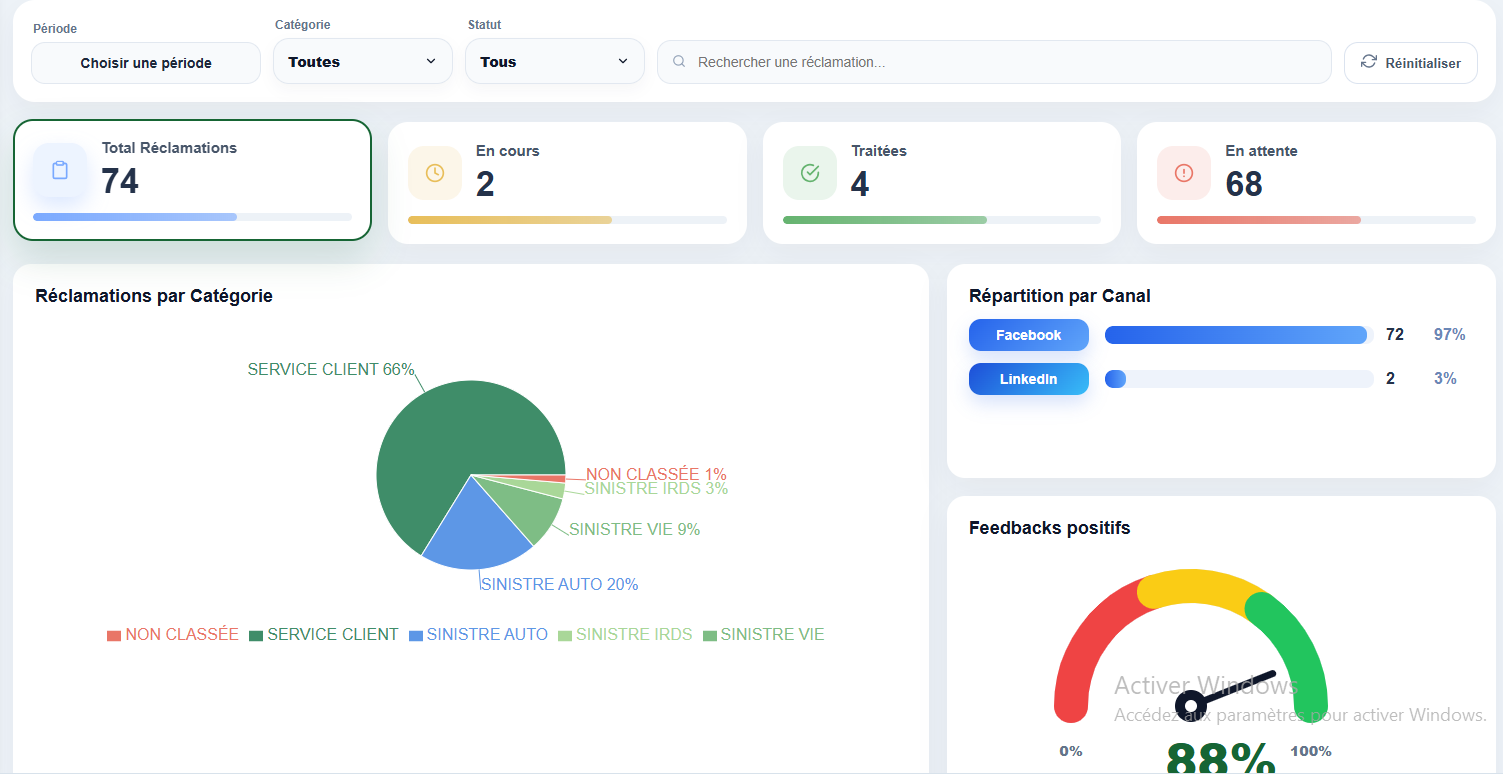
\includegraphics[width=1\linewidth]{dashboard_interface.png}
    \caption{Vue synthétique du dashboard BI}
\end{figure}

\begin{figure}[H]
    \centering
    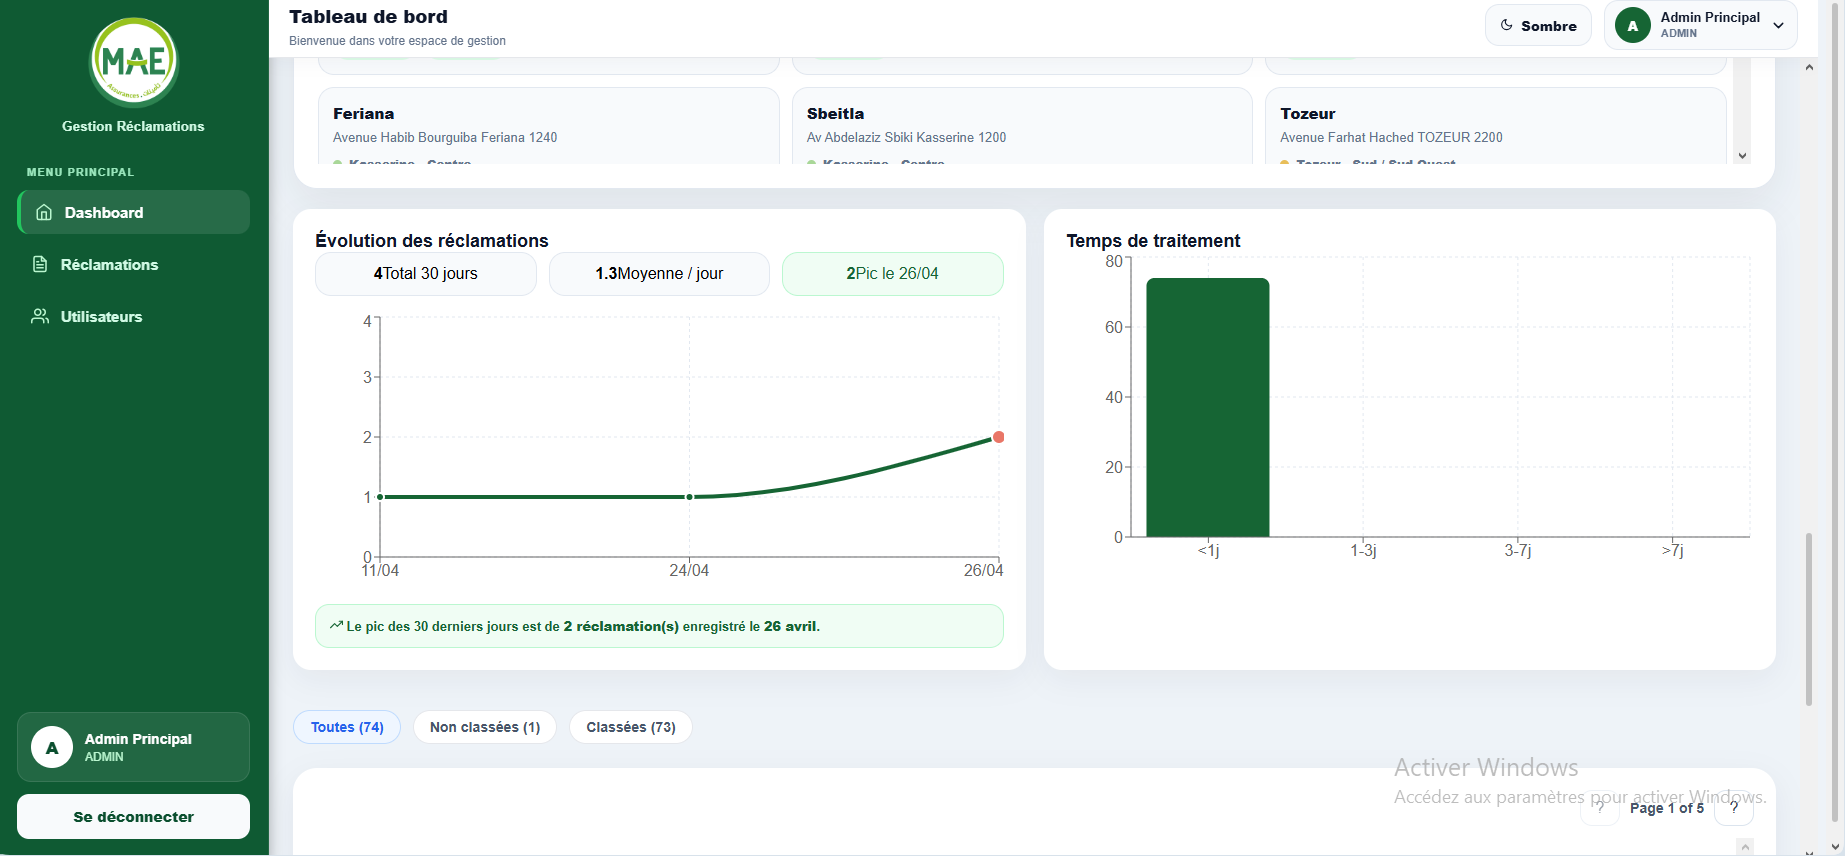
\includegraphics[width=1\linewidth]{analyse_dashboard.png}
    \caption{Analyse visuelle des réclamations}
\end{figure}

\begin{figure}[H]
    \centering
    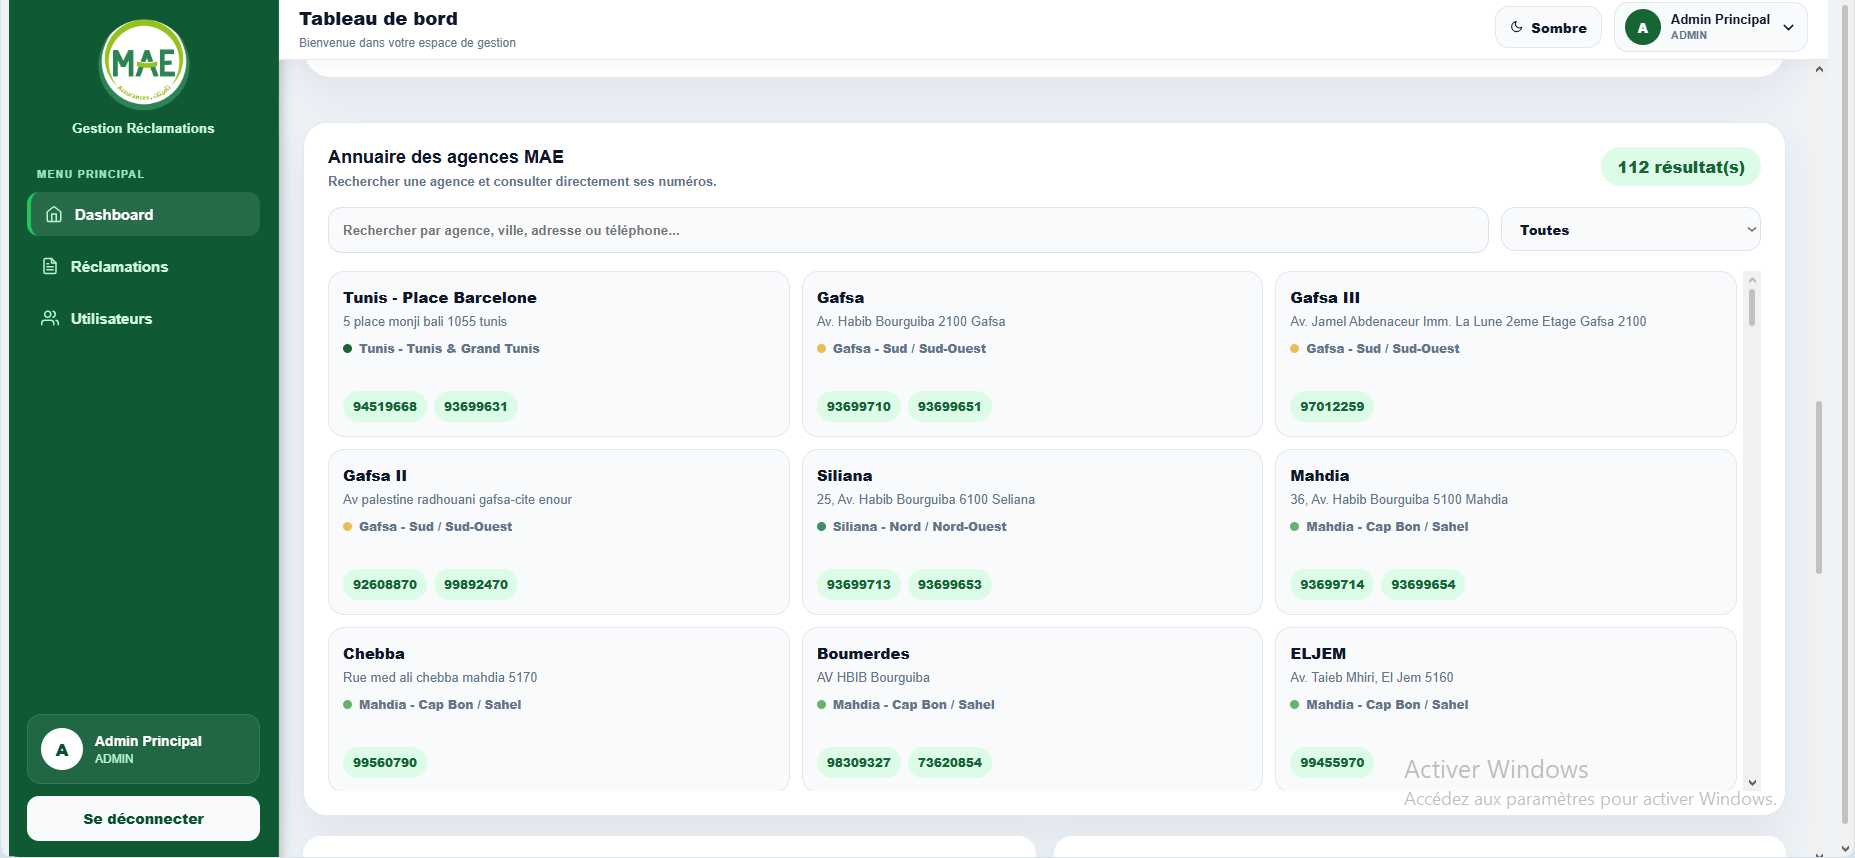
\includegraphics[width=1\linewidth]{annuaire_agences.png}
    \caption{Annuaire et répartition des agences}
\end{figure}

\begin{figure}[H]
    \centering
    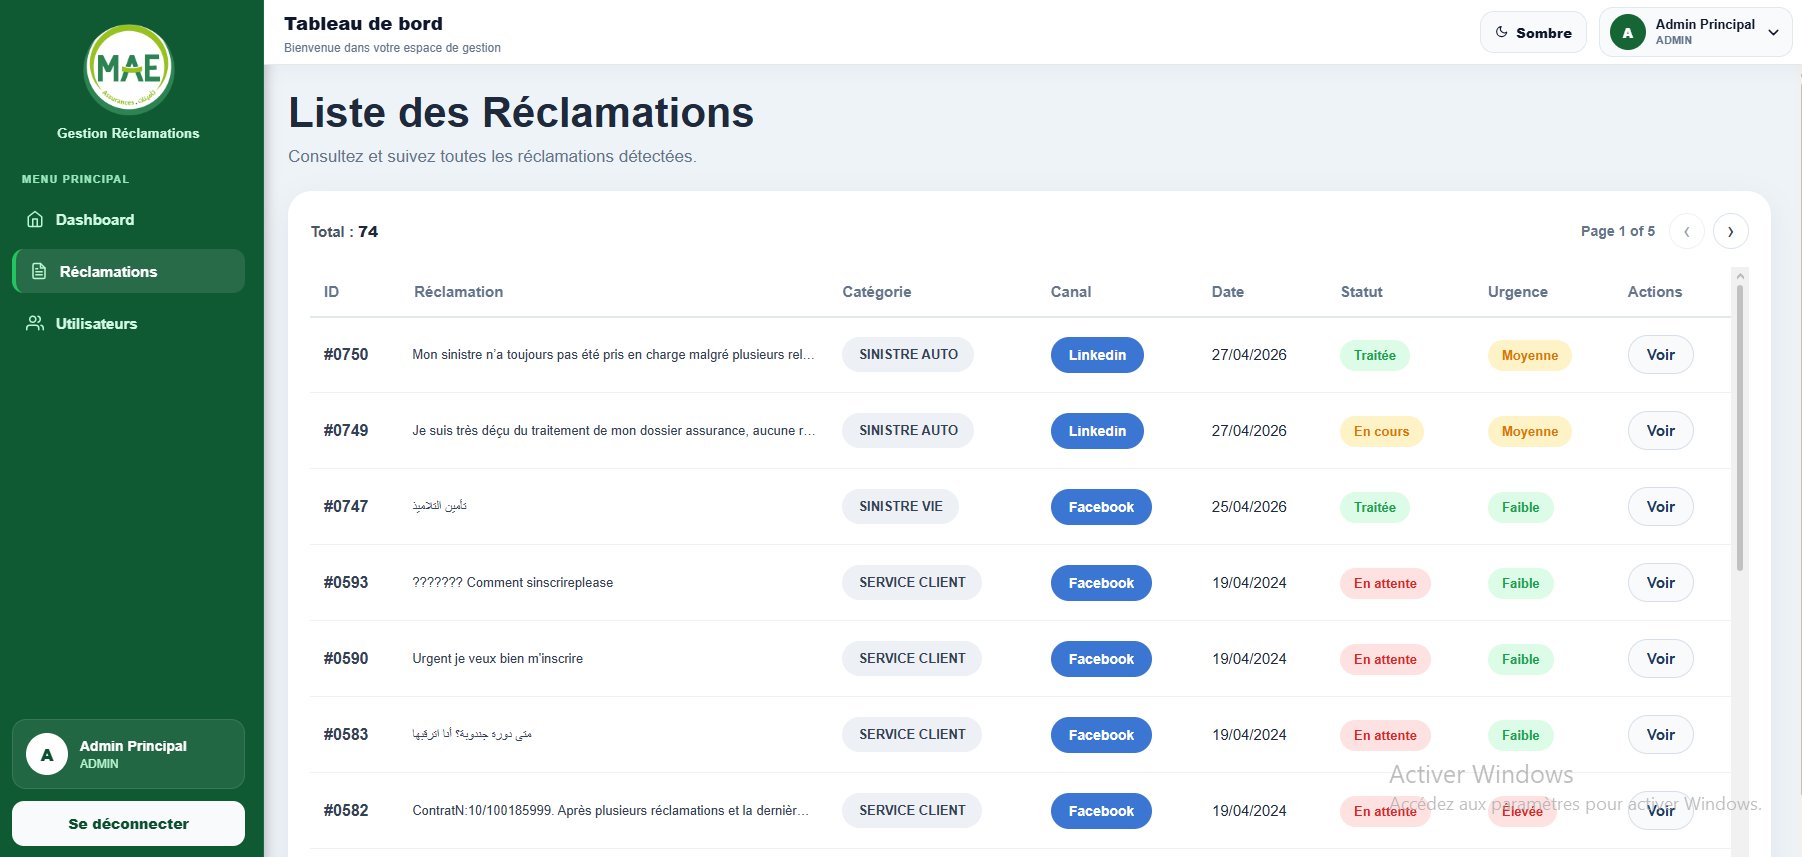
\includegraphics[width=1\linewidth]{table_reclamations2.png}
    \caption{Tableau de suivi des réclamations}
\end{figure}

\begin{figure}[H]
    \centering
    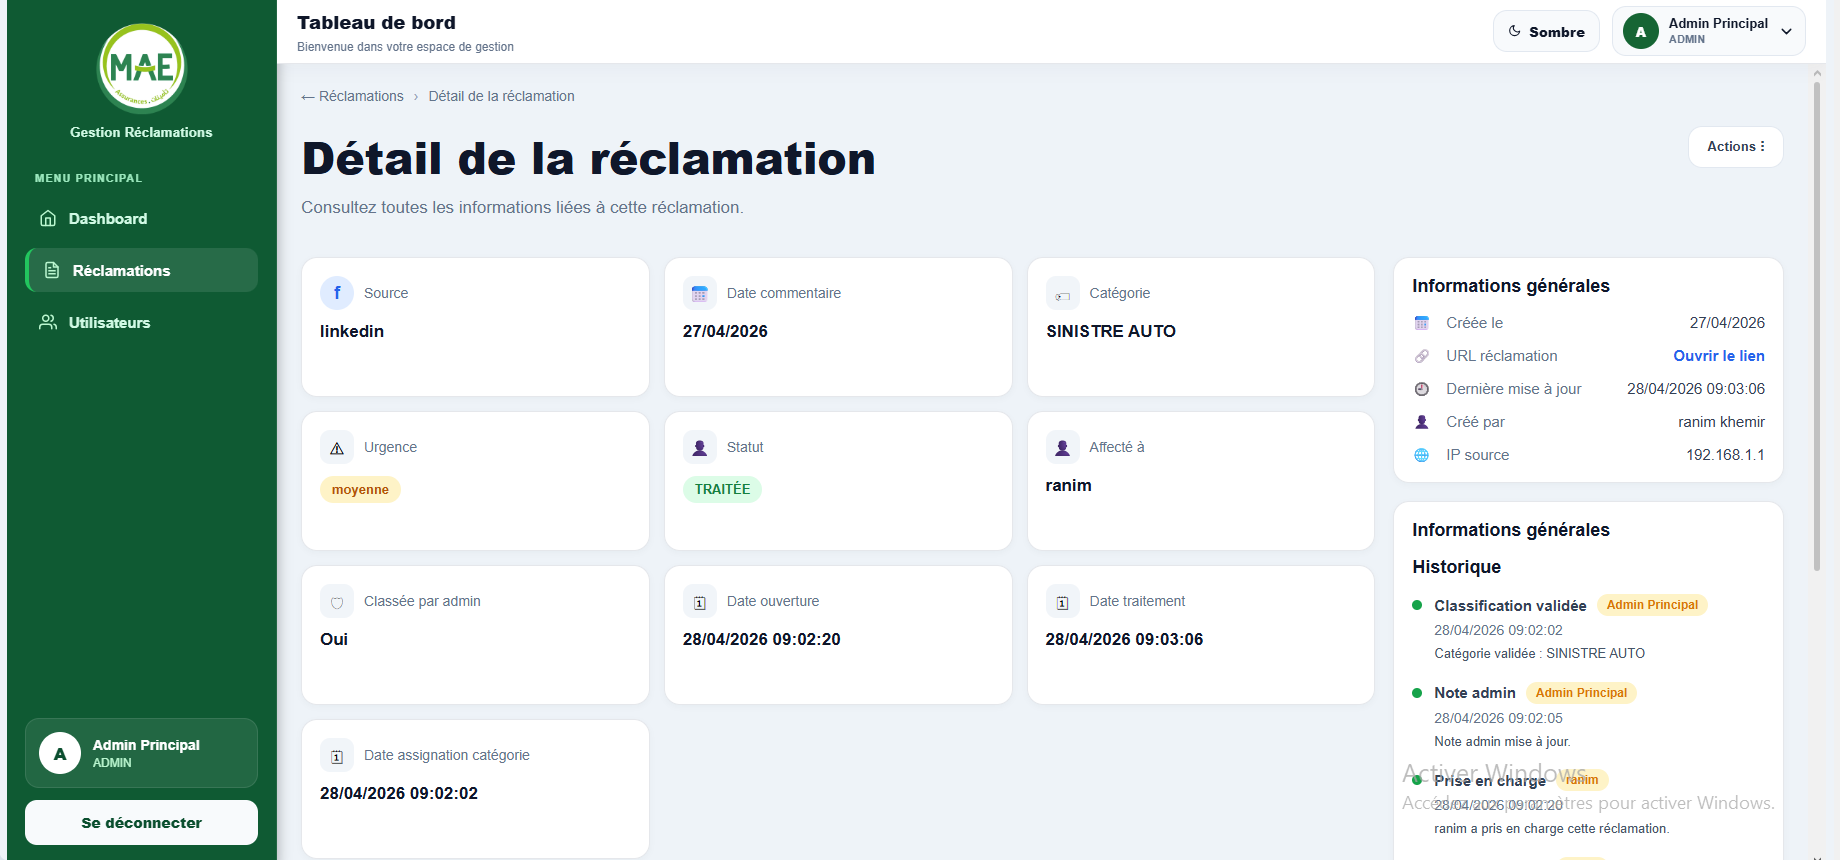
\includegraphics[width=1\linewidth]{detail_reclamation_1.png}
    \caption{Détail d’une réclamation}
\end{figure}

Cette visualisation permet à l’administrateur et aux agents d’avoir une vision globale de l’activité, d’identifier les catégories les plus fréquentes et de prioriser les actions selon le niveau d’urgence.


\section{KPI}
Les KPI (Key Performance Indicators), ou indicateurs clés de performance, permettent de mesurer et de suivre l’activité de la plateforme. Dans le cadre de ce projet, ils sont utilisés pour donner une vision synthétique de l’état des réclamations et faciliter la prise de décision.

\textbf{Les principaux KPI utilisés sont :}

\begin{itemize}
    \item \textbf{Nombre total de commentaires analysés :} il représente le nombre total de commentaires ayant été traités par le module NLP, en regroupant les réclamations détectées et les commentaires non réclamants.
    \item \textbf{Nombre total de réclamations :} il indique le nombre de commentaires identifiés comme des réclamations après traitement NLP.

    \begin{figure}[H]
        \centering
        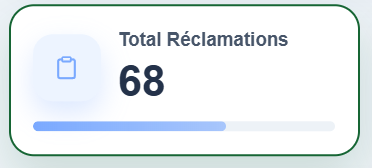
\includegraphics[width=0.3\linewidth]{Screenshot 2026-05-10 210335.png}
    \end{figure}
    
    \item \textbf{Nombre de commentaires non réclamants :} il permet de distinguer les avis positifs, les compliments ou les messages ne nécessitant pas de traitement.

    \begin{figure}[H]
        \centering
        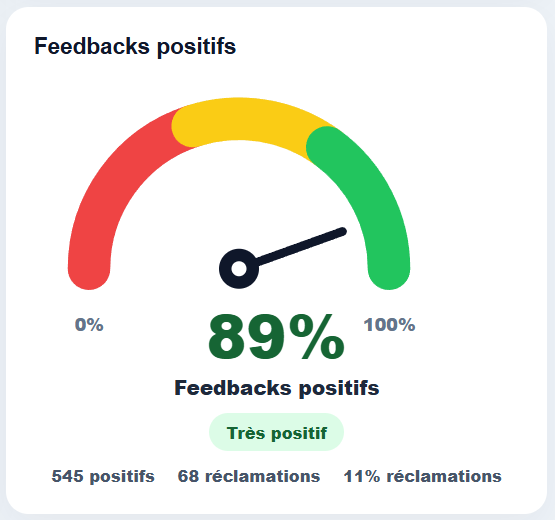
\includegraphics[width=0.3\linewidth]{Screenshot 2026-05-10 234446.png}
    \end{figure}
    
    \item \textbf{Réclamations en attente :} cet indicateur représente les réclamations détectées mais pas encore prises en charge.

    \begin{figure}[H]
        \centering
        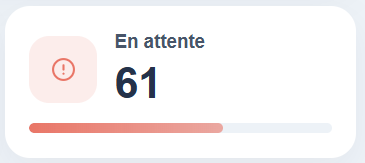
\includegraphics[width=0.3\linewidth]{Screenshot 2026-05-10 210408.png}
    \end{figure}
    
    \item \textbf{Réclamations en cours :} il indique les réclamations actuellement traitées par les agents.

    \begin{figure}[H]
        \centering
        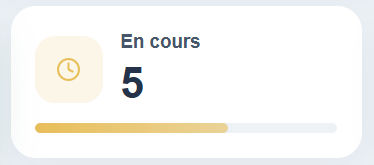
\includegraphics[width=0.3\linewidth]{Screenshot 2026-05-10 210348.png}
    \end{figure}
    
    \item \textbf{Réclamations traitées :} il correspond aux réclamations clôturées ou marquées comme traitées.

    \begin{figure}[H]
        \centering
        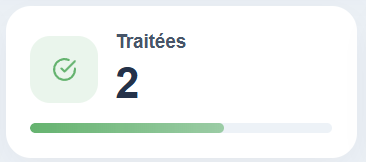
\includegraphics[width=0.3\linewidth]{Screenshot 2026-05-10 210358.png}
    \end{figure}
    
    \item \textbf{Répartition par catégorie :} cet indicateur permet d’identifier les domaines les plus concernés par les réclamations, par exemple Service Client, Sinistre Auto, Sinistre IRDS ou Sinistre Vie.

    \begin{figure}[H]
        \centering
        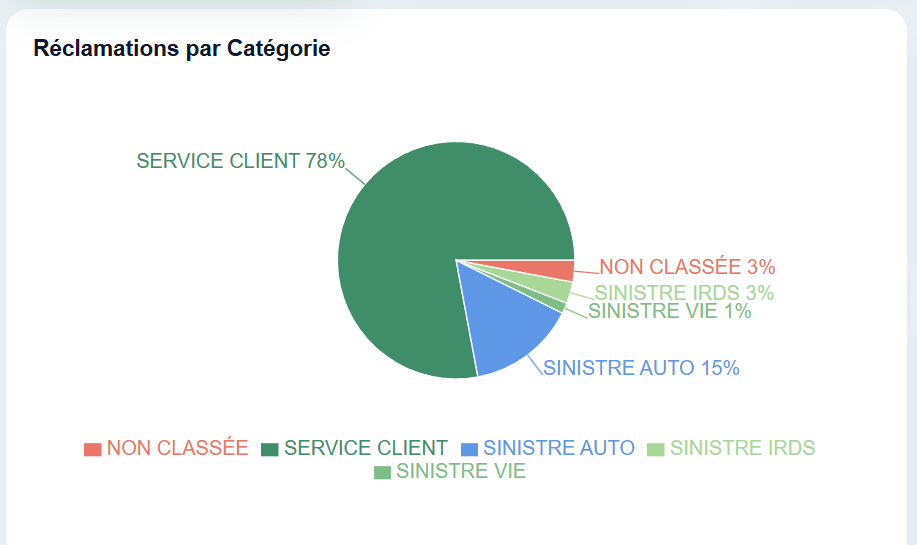
\includegraphics[width=0.5\linewidth]{Screenshot 2026-05-10 235405.png}
    \end{figure}
        \item \textbf{Répartition par niveau d’urgence :} elle permet de prioriser les actions selon le degré d’urgence des réclamations : faible, moyenne ou élevée.

    \begin{figure}[H]
        \centering
        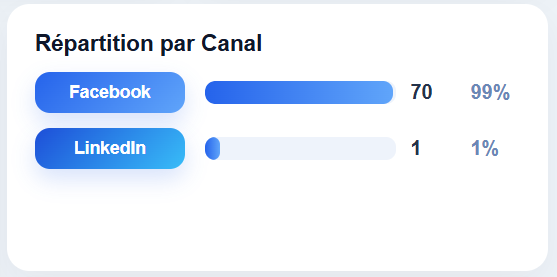
\includegraphics[width=0.4\linewidth]{Screenshot 2026-05-11 214927.png}
    \end{figure}
    
    \item \textbf{Répartition par source :} cet indicateur montre la provenance des commentaires, notamment Facebook ou LinkedIn.

    \begin{figure}[H]
        \centering
        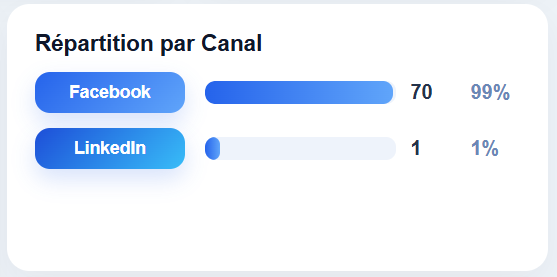
\includegraphics[width=0.4\linewidth]{Screenshot 2026-05-11 214927.png}
    \end{figure}
    
\end{itemize}

Ces indicateurs sont affichés dans le dashboard sous forme de cartes, de graphiques et de statistiques. Ils permettent à l’administrateur et aux agents d’avoir une vision globale de l’activité, de suivre l’évolution des réclamations et d’identifier rapidement les problèmes les plus fréquents ou les plus urgents.



\section{Tests et validation}

La validation du système a été réalisée à plusieurs niveaux afin de vérifier le bon fonctionnement des modèles, du module NLP et des API backend.

Tout d’abord, les modèles de Machine Learning ont été évalués à partir d’un découpage du dataset en données d’entraînement et données de test selon une répartition \textbf{80\% / 20\%}. Les métriques utilisées sont l’accuracy, la précision, le rappel et le F1-score.

Ensuite, le module NLP hybride a été testé sur \textbf{5 commentaires représentatifs}. Ces commentaires couvrent plusieurs cas : réclamation liée au service client, commentaire non réclamant, sinistre auto, demande d’information et réclamation ambiguë. L’objectif est de vérifier que le système retourne correctement le type du commentaire, la catégorie, le niveau d’urgence, la source de décision ainsi que le statut de validation.

L’extrait suivant présente la logique utilisée pour tester le module NLP. Le commentaire est d’abord analysé par la fonction hybride. Si une validation supplémentaire est nécessaire, le LLM-as-a-Judge intervient. Enfin, le résultat obtenu est comparé au résultat attendu afin d’afficher le statut \texttt{SUCCESS} ou \texttt{FAILED}.

Les tests du module NLP ont été réalisés à partir de scénarios représentatifs afin de vérifier la détection des réclamations, la classification de leur catégorie et l’estimation de leur niveau d’urgence.

Enfin, des tests fonctionnels ont été réalisés sur les principales API du backend Django. Ces tests vérifient l’authentification, la consultation des réclamations, la modification des notes, la classification manuelle, le changement de statut, la récupération des statistiques et la gestion des utilisateurs.

Pour les tests backend, chaque requête HTTP est comparée à un code de statut attendu. Si le code retourné par l’API correspond au code attendu, le test est considéré comme réussi et le script affiche \texttt{SUCCESS}.

Les tests backend vérifient la conformité des réponses HTTP retournées par les principales routes de l’API.

\begin{table}[H]
\centering
\small
\caption{Synthèse des tests fonctionnels backend}
\begin{tabular}{|p{4cm}|p{4cm}|p{4cm}|}
\hline
\textbf{Fonction testée} & \textbf{Route concernée} & \textbf{Résultat attendu} \\
\hline
Connexion valide & \path{/api/login/} & Authentification réussie et retour des informations utilisateur. \\
\hline
Connexion invalide & \path{/api/login/} & Refus de connexion. \\
\hline
Liste des réclamations & \path{/api/reclamations/} & Retour de la liste des réclamations. \\
\hline
Détail d’une réclamation & \path{/api/reclamations/<id>/} & Retour des informations détaillées. \\
\hline
Ajout d’une note interne & \path{/api/reclamations/<id>/internal-note/} & Note interne enregistrée. \\
\hline
Ajout d’une note administrative & \path{/api/reclamations/<id>/admin-note/} & Note administrative enregistrée. \\
\hline
Classification manuelle & \path{/api/reclamations/<id>/classify/} & Catégorie mise à jour. \\
\hline
Marquer comme traitée & \path{/api/reclamations/<id>/mark-processed/} & Statut de la réclamation mis à jour. \\
\hline
Statistiques dashboard & \path{/api/feedback-stats/} & Retour des indicateurs statistiques. \\
\hline
Liste des utilisateurs & \path{/api/users/} & Retour de la liste des utilisateurs. \\
\hline
Création utilisateur & \path{/api/users/} & Nouvel utilisateur créé. \\
\hline
Modification utilisateur & \path{/api/users/<id>/} & Informations utilisateur modifiées. \\
\hline
Suppression utilisateur & \path{/api/users/<id>/} & Compte supprimé ou désactivé. \\
\hline
\end{tabular}
\end{table}

Les tests réalisés montrent que les principales fonctionnalités du backend répondent correctement aux requêtes HTTP et retournent des données structurées au format JSON. Les résultats obtenus confirment le bon fonctionnement général de l’application dans le cadre de la version développée.

\section{Discussion des résultats}
Les résultats obtenus montrent que l’approche proposée permet d’automatiser efficacement une partie importante du traitement des réclamations. Le système arrive globalement à distinguer les réclamations des commentaires non réclamants, ce qui facilite l’identification rapide des messages nécessitant un suivi.

La classification des catégories donne également des résultats satisfaisants, notamment pour les catégories les plus représentées dans le dataset. Certaines catégories restent toutefois plus difficiles à reconnaître, en particulier lorsqu’elles disposent de moins d’exemples ou lorsque les commentaires contiennent peu d’indices explicites sur le domaine concerné.

L’estimation du niveau d’urgence représente une tâche plus complexe. Les niveaux d’urgence clairement exprimés sont généralement plus faciles à identifier, tandis que les situations intermédiaires peuvent être plus ambiguës. Cette difficulté s’explique par la nature subjective de l’urgence et par la diversité des formulations utilisées par les clients.

Ces observations confirment l’intérêt de l’approche hybride adoptée dans le projet. Le Machine Learning permet de traiter rapidement les cas simples ou suffisamment confiants. Le LLM intervient lorsque le contexte nécessite une analyse plus approfondie, tandis que le LLM-as-a-Judge permet de renforcer la validation des résultats incertains ou non classés.

Cependant, certaines limites restent présentes. Les performances dépendent fortement de la qualité du dataset, de son équilibre entre les classes et de la diversité linguistique des commentaires. Les textes courts, bruités, rédigés en dialecte ou contenant peu d’informations restent plus difficiles à classifier.

Ainsi, les résultats sont globalement encourageants pour une première version du système. Des améliorations peuvent être envisagées, notamment l’enrichissement du dataset, l’ajout de nouvelles données réelles, l’amélioration du prétraitement multilingue et l’ajustement des seuils de confiance utilisés dans la route hybride.

En résumé, le système atteint son objectif principal : détecter automatiquement les réclamations, proposer une catégorie et estimer leur urgence, tout en conservant un mécanisme de validation pour les cas incertains.

\section{Conclusion}
Dans ce chapitre, nous avons présenté le traitement intelligent appliqué aux réclamations, depuis l’exploration des données jusqu’à l’entraînement et l’évaluation des modèles. Les résultats obtenus montrent que les modèles ML permettent d’automatiser la détection des réclamations, la classification des catégories et l’estimation de l’urgence avec des performances satisfaisantes. L’approche hybride combinant ML, LLM et LLM-as-a-Judge permet de renforcer la fiabilité du système, notamment dans les cas incertains ou ambigus. Enfin, l’exploitation des résultats dans le dashboard BI facilite le suivi des réclamations et l’aide à la décision.


% ===== CONCLUSION GENERALE =====
\chapter*{Conclusion générale}
\addcontentsline{toc}{chapter}{Conclusion générale}

Au terme de ce projet, nous avons conçu et développé une plateforme intelligente dédiée à la collecte, l’analyse et la gestion des réclamations clients. Cette solution permet de centraliser les commentaires collectés depuis les réseaux sociaux, de les préparer à travers des étapes de nettoyage et de prétraitement, puis de les exploiter à l’aide d’un module NLP.

Le système développé repose sur une architecture modulaire intégrant une interface web React, un backend Django REST Framework, une base de données PostgreSQL et un module intelligent de classification. L’approche hybride adoptée combine des modèles de Machine Learning, un modèle de langage LLM et un mécanisme LLM-as-a-Judge afin d’améliorer la fiabilité des prédictions et de traiter les cas incertains.

La plateforme permet également aux agents et à l’administrateur de consulter les réclamations, suivre leur état, ajouter des notes, effectuer une classification manuelle si nécessaire et visualiser les indicateurs à travers un dashboard BI. Les tests réalisés ont permis de valider le fonctionnement des modèles, du module NLP et des principales API backend.

Malgré les résultats encourageants, certaines limites demeurent. La performance du système dépend fortement de la qualité et de la diversité des données collectées. Les commentaires courts, ambigus, bruités ou rédigés en dialecte peuvent encore poser des difficultés de classification. De plus, certaines catégories nécessitent davantage d’exemples afin d’améliorer la précision des modèles.

Comme perspectives, il serait intéressant d’enrichir le dataset avec davantage de données réelles, d’améliorer le traitement multilingue, d’ajuster les seuils de confiance de la route hybride, d’intégrer de nouvelles sources de collecte et de renforcer la sécurité pour un déploiement en environnement réel. Ce projet constitue ainsi une première version fonctionnelle d’une solution intelligente d’aide au traitement et au suivi des réclamations clients.


% ===== BIBLIOGRAPHIE =====
\begin{thebibliography}{99}
\addcontentsline{toc}{chapter}{Bibliographie}
\bibitem{mae}
MAE Assurances, \textit{Présentation de l’entreprise}, disponible sur : \url{https://www.mae.tn/}
\bibitem{crispdm}
P. Chapman et al., \textit{CRISP-DM 1.0: Step-by-step data mining guide}, 2000.
\bibitem{zendesk}
Zendesk, \textit{Customer Service Software}, disponible sur : \url{https://www.zendesk.com/}

\bibitem{salesforce}
Salesforce, \textit{Service Cloud}, disponible sur : \url{https://www.salesforce.com/products/service-cloud/}

\bibitem{freshdesk}
Freshdesk, \textit{Customer Support Software}, disponible sur : \url{https://www.freshworks.com/freshdesk/}

\bibitem{tfidf}
Documentation scikit-learn, Feature Extraction, disponible sur : \url{https://scikit-learn.org/stable/modules/feature_extraction.html}
\bibitem{ibmnlp}
IBM, \textit{What is Natural Language Processing (NLP)?}, disponible sur : \url{https://www.ibm.com/topics/natural-language-processing}
\bibitem{drf}
Django REST Framework, \textit{Official Documentation}, disponible sur : \url{https://www.django-rest-framework.org/}
\bibitem{react}
React, \textit{Official Documentation}, disponible sur : \url{https://react.dev/}
\bibitem{postgresql}
PostgreSQL Global Development Group, \textit{PostgreSQL Documentation}, disponible sur : \url{https://www.postgresql.org/docs/}
\bibitem{fastapi}
FastAPI, \textit{Official Documentation}, disponible sur : \url{https://fastapi.tiangolo.com/}
\bibitem{scikitlearn}
Scikit-learn developers, \textit{Scikit-learn Documentation}, disponible sur : \url{https://scikit-learn.org/stable/}
\bibitem{logreg}
Scikit-learn developers, \textit{LogisticRegression}, disponible sur : \url{https://scikit-learn.org/stable/modules/generated/sklearn.linear_model.LogisticRegression.html}
\bibitem{ibmllm}
IBM, \textit{What are Large Language Models (LLMs)?}, disponible sur : \url{https://www.ibm.com/topics/large-language-models}
\bibitem{hftransformers}
Hugging Face, \textit{Transformers Documentation}, disponible sur : \url{https://huggingface.co/docs/transformers/}
\bibitem{ibmeval}
IBM, \textit{LLM Evaluation}, disponible sur : \url{https://www.ibm.com/think/insights/llm-evaluation}
\bibitem{jwtio}
JWT.io, \textit{Introduction to JSON Web Tokens}, disponible sur : \url{https://jwt.io/introduction/}
\bibitem{mdncors}
MDN Web Docs, \textit{Cross-Origin Resource Sharing (CORS)}, disponible sur : \url{https://developer.mozilla.org/en-US/docs/Web/HTTP/Guides/CORS}
\bibitem{metrics}
Scikit-learn developers, \textit{Model evaluation: quantifying the quality of predictions}, disponible sur : \url{https://scikit-learn.org/stable/modules/model_evaluation.html}
\end{thebibliography}

% ===== ANNEXES =====
\appendix
\chapter{Annexes}

\section{Diagrammes UML}
Cette annexe présente une synthèse des principaux diagrammes UML utilisés dans le cadre de la conception de la plateforme. Ces diagrammes ont permis de représenter les fonctionnalités attendues, la structure du système et les interactions entre ses différents composants.

\begin{table}[H]
\centering
\small
\caption{Synthèse des diagrammes UML réalisés}
\label{tab:annexe_uml}
\begin{tabular}{|p{4cm}|p{9cm}|}
\hline
\textbf{Diagramme} & \textbf{Objectif} \\
\hline
Diagramme de cas d'utilisation général & Présenter les interactions principales entre les acteurs du système, notamment l'agent et l'administrateur. \\
\hline
Diagramme de cas d'utilisation détaillé & Décrire plus précisément les fonctionnalités offertes par la plateforme, telles que la consultation, le filtrage, le traitement et la classification des réclamations. \\
\hline
Diagramme de classes & Représenter la structure statique du système à travers les entités principales : utilisateur, commentaire, annotation, réclamation et journal des actions. \\
\hline
Diagrammes de séquence & Illustrer le déroulement des principaux scénarios, comme la consultation des réclamations, le traitement d'une réclamation, l'affichage du dashboard et la classification automatique via le module NLP. \\
\hline
\end{tabular}
\end{table}

Les diagrammes UML ont été réalisés afin de faciliter la compréhension du système avant son implémentation. Ils ont également servi de base pour organiser les modules de l'application, définir les relations entre les données et préciser les responsabilités de chaque composant.

\subsection{Règles de gestion principales}

Les règles de gestion suivantes ont été retenues pour assurer le bon fonctionnement de la plateforme :

\begin{enumerate}
    \item Chaque utilisateur doit s'authentifier avant d'accéder aux fonctionnalités de la plateforme.
    \item Un administrateur peut gérer les comptes utilisateurs et classifier manuellement une réclamation si nécessaire.
    \item Un agent peut consulter les réclamations, ajouter des notes internes et modifier leur statut.
    \item Une réclamation peut avoir trois statuts principaux : en attente, en cours ou traitée.
    \item Les commentaires détectés comme réclamations sont associés à une catégorie et à un niveau d'urgence.
    \item Les actions effectuées sur une réclamation sont enregistrées afin d'assurer la traçabilité.
\end{enumerate}

\section{Documentation API}
Cette section présente les principales routes API exposées par le backend Django REST Framework. Les routes sont utilisées par l'interface React pour gérer l'authentification, les utilisateurs, les réclamations et les statistiques du dashboard.

\begin{table}[H]
\centering
\scriptsize
\caption{Routes API d'authentification et de gestion des utilisateurs}
\label{tab:annexe_api_users}
\begin{tabular}{|p{1.8cm}|p{5.7cm}|p{5.7cm}|}
\hline
\textbf{Méthode} & \textbf{Route} & \textbf{Description} \\
\hline
POST & \path{/api/login/} & Authentifier un utilisateur et retourner les informations de session. \\
\hline
POST & \path{/api/change-password/} & Permettre à un utilisateur de modifier son mot de passe. \\
\hline
POST & \path{/api/forgot-password/} & Générer un mot de passe provisoire et envoyer un email de récupération. \\
\hline
GET & \path{/api/users/} & Récupérer la liste des utilisateurs. \\
\hline
POST & \path{/api/users/} & Créer un nouveau compte utilisateur. \\
\hline
PUT & \path{/api/users/<id>/} & Modifier les informations d'un utilisateur existant. \\
\hline
DELETE & \path{/api/users/<id>/} & Supprimer ou désactiver un utilisateur. \\
\hline
\end{tabular}
\end{table}

\begin{table}[H]
\centering
\scriptsize
\caption{Routes API de gestion des réclamations et des statistiques}
\label{tab:annexe_api_reclamations}
\begin{tabular}{|p{1.8cm}|p{5.9cm}|p{5.5cm}|}
\hline
\textbf{Méthode} & \textbf{Route} & \textbf{Description} \\
\hline
GET & \path{/api/reclamations/} & Récupérer la liste des réclamations détectées. \\
\hline
GET & \path{/api/reclamations/<id>/} & Consulter les détails d'une réclamation. \\
\hline
PATCH & \path{/api/reclamations/<id>/internal-note/} & Ajouter ou modifier une note interne sur une réclamation. \\
\hline
PATCH & \path{/api/reclamations/<id>/admin-note/} & Ajouter une note administrative liée à la classification. \\
\hline
PATCH & \path{/api/reclamations/<id>/classify/} & Modifier manuellement la catégorie d'une réclamation. \\
\hline
PATCH & \path{/api/reclamations/<id>/mark-processed/} & Marquer une réclamation comme traitée. \\
\hline
GET & \path{/api/feedback-stats/} & Récupérer les statistiques utilisées dans le dashboard. \\
\hline
\end{tabular}
\end{table}

\subsection{Champs principaux retournés pour une réclamation}

\begin{table}[H]
\centering
\small
\caption{Champs principaux d'une réclamation}
\label{tab:annexe_champs_reclamation}
\begin{tabular}{|p{4cm}|p{9cm}|}
\hline
\textbf{Champ} & \textbf{Description} \\
\hline
\texttt{id} & Identifiant de la réclamation. \\
\hline
\texttt{source} & Source du commentaire, par exemple Facebook ou LinkedIn. \\
\hline
\texttt{text\_original} & Texte original du commentaire collecté. \\
\hline
\texttt{category} & Catégorie attribuée à la réclamation : Service Client, Sinistre Auto, Sinistre IRDS ou Sinistre Vie. \\
\hline
\texttt{urgency} & Niveau d'urgence estimé : faible, moyenne ou élevée. \\
\hline
\texttt{status} & État de traitement de la réclamation : EN\_ATTENTE, EN\_COURS ou TRAITEE. \\
\hline
\texttt{assigned\_agent} & Agent chargé du traitement de la réclamation. \\
\hline
\texttt{internal\_note} & Note ajoutée par l'agent pour assurer le suivi. \\
\hline
\texttt{action\_logs} & Historique des actions effectuées sur la réclamation. \\
\hline
\end{tabular}
\end{table}

\section{Exemples de données}
Les données utilisées dans ce projet sont principalement des commentaires textuels collectés ou simulés à partir de sources sociales. Après nettoyage, elles sont structurées afin d'être exploitées par le module NLP et par les modèles de classification.

\subsection{Exemple de commentaire après prétraitement}

\begin{table}[H]
\centering
\small
\caption{Exemples de commentaires utilisés dans le dataset}
\label{tab:annexe_exemples_donnees}
\begin{tabular}{|p{7cm}|p{3cm}|p{3cm}|}
\hline
\textbf{Texte nettoyé} & \textbf{Type} & \textbf{Catégorie} \\
\hline
agence mourouj merci je suis très satisfaite & non\_reclamation & NULL \\
\hline
assurance dun véhicule à deux roues moto coûts élevés & reclamation & SINISTRE AUTO \\
\hline
désolé mais ceci na rien changé je ne recois pas toujours des code dactivation & reclamation & SERVICE CLIENT \\
\hline
\end{tabular}
\end{table}

\subsection{Répartition du dataset}

Le dataset utilisé pour l'entraînement contient \textbf{484 commentaires}. Il est composé de \textbf{243 réclamations} et de \textbf{241 commentaires non réclamants}.

\begin{table}[H]
\centering
\small
\caption{Répartition des catégories de réclamations}
\label{tab:annexe_repartition_categories}
\begin{tabular}{|p{6cm}|p{4cm}|}
\hline
\textbf{Catégorie} & \textbf{Nombre d'exemples} \\
\hline
SERVICE CLIENT & 81 \\
\hline
SINISTRE IRDS & 56 \\
\hline
SINISTRE VIE & 54 \\
\hline
SINISTRE AUTO & 52 \\
\hline
\end{tabular}
\end{table}

\subsection{Exemple de résultat NLP}

Après analyse par le module NLP, chaque commentaire est enrichi avec des informations permettant son exploitation dans la plateforme.

\begin{verbatim}
{
  "result": {
    "is_reclamation": "reclamation",
    "category": "SINISTRE AUTO",
    "urgency": "moyenne",
    "source": "ml"
  },
  "processing_status": "no_judge"
}
\end{verbatim}

Ce résultat permet au backend de créer une réclamation, de l'afficher dans l'interface et de l'intégrer dans les indicateurs du dashboard.

\end{document}
